\documentclass[%
11pt,%
%oneside,%
twoside,%
%twocolumn,%
titlepage,%
%fleqn,%
%a4page,%
german,%
headsepline%
]{scrartcl}

%\usepackage{fancyhdr}
%\usepackage{scrpage2}
\usepackage{lastpage}
\usepackage{geometry}
\usepackage{graphicx}
\usepackage[utf8]{inputenc}
\usepackage[ngerman]{babel}
\usepackage{lscape}
\usepackage[framemethod=TikZ]{mdframed}
\usepackage[most]{tcolorbox}
\usepackage{mymath}
\usepackage{units}
\usepackage{nicefrac}
\usepackage{pgf,tikz}
\usetikzlibrary{arrows}
\usepackage{colortbl}
\usepackage{hhline}
\usepackage{multirow}
\usepackage[extendedchars]{grffile}
\usepackage{caption}
\usepackage{multicol,calc}
\usepackage{blindtext}
\usepackage{pdfpages}
\usepackage{hyperref}
\usepackage{marginnote}
\usepackage{qrcode}
\qrset{height=9ex}
%\usepackage{tikz-er2}
\usepackage{framed}
\usetikzlibrary{arrows}
\usetikzlibrary{positioning}
\usetikzlibrary{shadows}

%\usepackage{romannum}
\usepackage{longtable}
\usepackage{listings}
\usepackage{wrapfig}


% Command, um Tabellen-Spalten anzupassen
\newcommand{\spaltenheight}{\rule{0mm}{3ex}}
\newcommand{\spaltenwidth}{\rule{3cm}{0mm}}
\newcommand{\spaltensep}{\\[1ex]}
%\arrayrulecolor{darkgreen}
\doublerulesepcolor{white}
\definecolor{lightyellow}{rgb}{1,1,0.8}
\definecolor{Gray}{gray}{0.9}


% Pagestyle/Layout
%\geometry{a4paper , tmargin =2.5cm,	bmargin=3cm, lmargin =2.5cm,	rmargin =2.5cm,	headheight=3em, headsep=1em, footskip=1cm}
\setlength{\parindent}{0pt} \setlength{\parskip}{1em}
%für TwoSide
%\lehead{\headmark\pagemark}
%\cehead{}
%\rehead{}
%\lohead{}
%\cohead{}
%\rohead{\headmark}
%für OneSide
%\ihead{}
%\chead{}
%\ohead{}
%\setheadsepline{0.5pt} % Linie zur Begrenzung
%\setfootsepline{0.5pt} % Linie zur Begrenzung
\pagestyle{headings} % gemachte Einstellungen anwenden

% Farbig umrahmte Umgebung Satz
 
 \definecolor{myblizzardblue}{HTML}{87CEEB}

\newcounter{satzz}[section]\setcounter{satzz}{0}
\renewcommand{\thesatz}{\arabic{section}.\arabic{satzz}}

\newenvironment{csatz}[2][]{%
    \refstepcounter{satzz}
 
    \ifstrempty{#1}%
    % if condition (without title)
    {\mdfsetup{%
        frametitle={%
            \tikz[baseline=(current bounding box.east),outer sep=0pt]
            \node[anchor=east,rectangle,fill=myblizzardblue]
            {\strut Satz~\thesatz};}
        }%
    % else condition (with title)
    }{\mdfsetup{%
        frametitle={%
            \tikz[baseline=(current bounding box.east),outer sep=0pt]
            \node[anchor=east,rectangle,fill=myblizzardblue]
            {\strut Satz~\thesatz:~#1};}%
        }%
    }%
% for both conditions
    \mdfsetup{%
        innertopmargin=10pt,linecolor=myblizzardblue,%
        backgroundcolor=whitesmoke,%
        linewidth=2pt,topline=true,%
        frametitleaboveskip=\dimexpr-\ht\strutbox\relax%
    }
 
\begin{mdframed}[]\relax}{%
\end{mdframed}}

% Farbig umrahmte Umgebung Theorem
 
\definecolor{mygraphblue}{HTML}{84B7E1}
\definecolor{whitesmoke}{HTML}{F5F5F5}

\newcounter{theo}[section]\setcounter{theo}{0}
\renewcommand{\thetheo}{\arabic{section}.\arabic{theo}}

\newenvironment{ctheo}[2][]{%
    \refstepcounter{theo}
 
    \ifstrempty{#1}%
    % if condition (without title)
    {\mdfsetup{%
        frametitle={%
            \tikz[baseline=(current bounding box.east),outer sep=0pt]
            \node[anchor=east,rectangle,fill=mygraphblue]
            {\strut Theorem~\thetheo};}
        }%
    % else condition (with title)
    }{\mdfsetup{%
        frametitle={%
            \tikz[baseline=(current bounding box.east),outer sep=0pt]
            \node[anchor=east,rectangle,fill=mygraphblue]
            {\strut Theorem~\thetheo:~#1};}%
        }%
    }%
% for both conditions
    \mdfsetup{%
        innertopmargin=10pt,linecolor=mygraphblue,%
        backgroundcolor=whitesmoke,%
        linewidth=2pt,topline=true,%
        frametitleaboveskip=\dimexpr-\ht\strutbox\relax%
    }
 
\begin{mdframed}[]\relax}{%
\end{mdframed}}

% Farbig umrahmte Umgebung Definition
 
 \definecolor{emerald}{HTML}{50C878}

\newcounter{deff}[section]\setcounter{deff}{0}
\renewcommand{\thedeff}{\arabic{section}.\arabic{deff}}

\newenvironment{cdef}[2][]{%
    \refstepcounter{deff}
 
    \ifstrempty{#1}%
    % if condition (without title)
    {\mdfsetup{%
        frametitle={%
            \tikz[baseline=(current bounding box.east),outer sep=0pt]
            \node[anchor=east,rectangle,fill=emerald]
            {\strut Definition~\thedeff};}
        }%
    % else condition (with title)
    }{\mdfsetup{%
        frametitle={%
            \tikz[baseline=(current bounding box.east),outer sep=0pt]
            \node[anchor=east,rectangle,fill=emerald]
            {\strut Definition~\thedeff:~#1};}%
        }%
    }%
% for both conditions
    \mdfsetup{%
        innertopmargin=10pt,linecolor=emerald,%
        backgroundcolor=whitesmoke,%
        linewidth=2pt,topline=true,%
        frametitleaboveskip=\dimexpr-\ht\strutbox\relax%
    }
 
\begin{mdframed}[]\relax}{%
\end{mdframed}}

% Farbig umrahmte Umgebung Achtung
 
 \definecolor{mygraphred}{HTML}{E26A6A}

\newcounter{merkee}[section]\setcounter{merkee}{0}
\renewcommand{\themerkee}{\arabic{section}.\arabic{merkee}}

\newenvironment{cachtung}[2][]{%
    \refstepcounter{merkee}
 
    \ifstrempty{#1}%
    % if condition (without title)
    {\mdfsetup{%
        frametitle={%
            \tikz[baseline=(current bounding box.east),outer sep=0pt]
            \node[anchor=east,rectangle,fill=mygraphred]
            {\strut Achtung};}
        }%
    % else condition (with title)
    }{\mdfsetup{%
        frametitle={%
            \tikz[baseline=(current bounding box.east),outer sep=0pt]
            \node[anchor=east,rectangle,fill=mygraphred]
            {\strut Achtung:~#1};}%
        }%
    }%
% for both conditions
    \mdfsetup{%
        innertopmargin=10pt,linecolor=mygraphred,%
        backgroundcolor=whitesmoke,%
        linewidth=2pt,topline=true,%
        frametitleaboveskip=\dimexpr-\ht\strutbox\relax%
    }
 
\begin{mdframed}[]\relax}{%
\end{mdframed}}

\subject{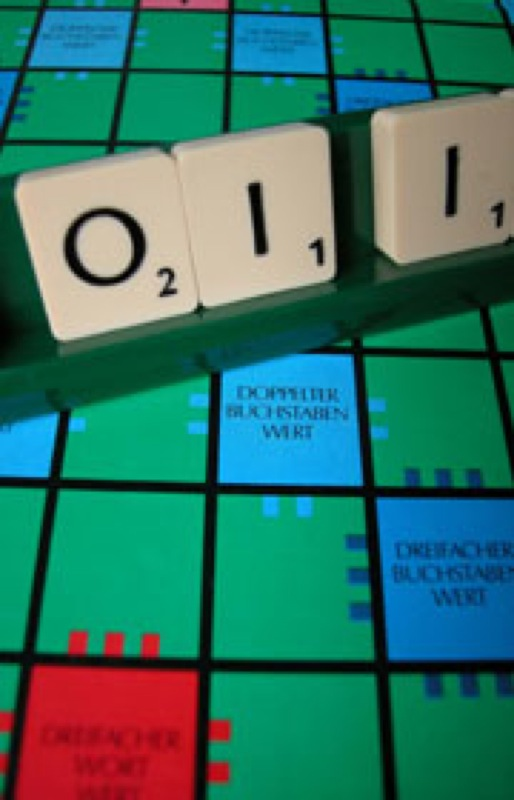
\includegraphics[width=0.38\textwidth]{pictures/scrabble}}
\title{Kryptologie}
\subtitle{Von Caesar bis RSA}
\author{}
\date{}
%\lowertitleback{
%\includegraphics[height=1.1cm]{/Users/jormawassmer/Pictures/logokoeniz.jpg}%
%\copyright Jorma Wassmer
%1. Auflage, Februar 2011
%}


\begin{document}
\maketitle

\newpage\thispagestyle{empty}~
\newpage

\tableofcontents
%\thispagestyle{empty}
\cleardoublepage
%\setcounter{page}{1}

\section{Geschichtliches zur Kryptologie}
\pagenumbering{arabic}
\begin{quote}
Kryptologie ist die Kunst und Wissenschaft, Methoden zur Verheimlichung von Nachrichten zu entwickeln.
\end{quote}

Häufig
\begin{wrapfigure}{r}{0.382\textwidth}
  \begin{center}
    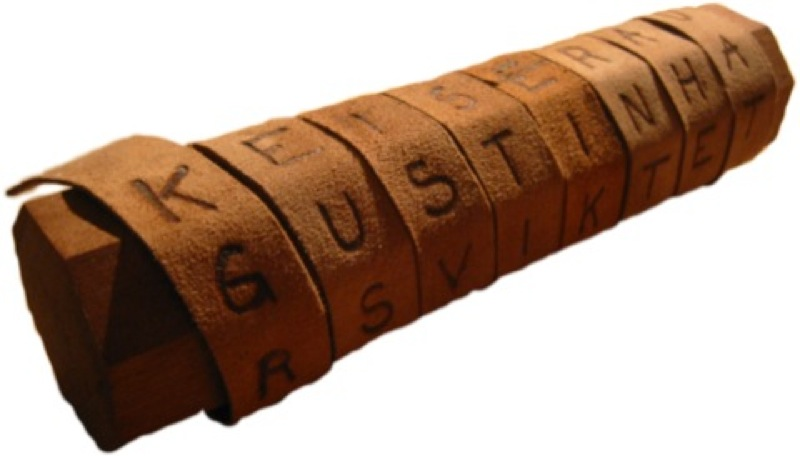
\includegraphics[width=0.38\textwidth]{pictures/skytale}
  \end{center}
%\caption{A gull}
\end{wrapfigure}
wird dabei noch zwischen Kryptographie --- der Wissenschaft von der Entwicklung von Kryptosystemen --- und Kryptoanalyse --- der Kunst des Brechens dieser Systeme --- unterschieden. Die Begriffe Kryptologie und Kryptographie sind aus dem griechischen W\"ortern $\kappa\gr\gy\pi\gt\go\gs$ (geheim) und $\gl\go\gg\go\gs$ (das Wort, die Lehre, der Sinn) gebildet.
Die \textbf{Kryptologie} beschäftigt sich mit der Ver- und Entschlüsselung von Informationen. Dieses Thema mutet zwar recht Antik an, wird aber in unserer zeit wieder verstärkt ben\"otigt, denkt man nur an die Sicherheit im Internet, an Chipkarten und Passw\"orter.

\subsection{Skytale}

Vor ungefähr 2500 Jahren verwendete die Regierung von Sparta eine trickreiche Methode zur übermittlung geheimer Nachrichten. Sender und Empfänger mussten beide einen sogenannten Skytale haben. Ein \textbf{Skytale} ist ein Zylinder mit einem bestimmten Durchmesser und vorgegebener Flächenzahl. Der Sender wickelte ein schmales Band aus Pergament spiralf\"ormig um seinen Zylinder und schrieb dann der Länge nach seine Nachricht auf das Band. War nun das Band abgewickelt, konnte die Nachricht mühelos von einer Person gelesen werden, die einen Zylinder genau desselben Umfangs hatte.

\subsection{Steganographie}

Auch die \textbf{Steganographie}, eine Art von gedeckten Geheimschriften war früh bekannt. Diese Geheimschriften konnten entweder als unverfängliche, offen verständliche Nachricht oder in (winzigen) sichtbaren graphischen Details einer Schrift oder Zeichnung erscheinen. Letzteres bezeichnete man auch als \textbf{Semagramm}.

\begin{figure}
\begin{center}
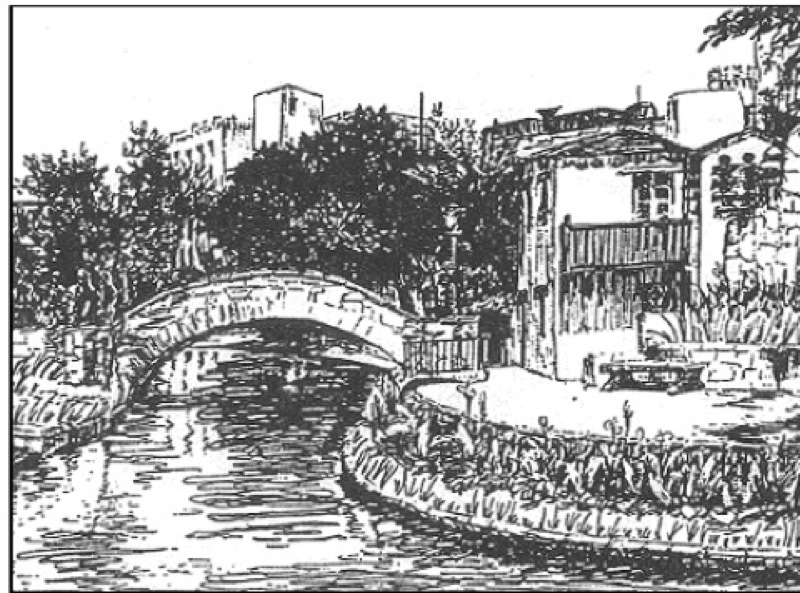
\includegraphics[width=1.2\textwidth, angle=90]{pictures/semabauer.jpg}
\caption{Semagramm mit Morsecode (aus Bauer)}\label{semagramm}
\end{center}
\end{figure}

Die Nachricht steht im Morsecode, der aus kurzen und langen Grashalmen links von der Brücke entlang des Flusses und auf der kleinen Mauer gebildet wird (siehe Abbildung \ref{semagramm} auf Seite \pageref{semagramm}).

\subsection{Caesar Cipher}

\textsc{Julius Caesar}
\marginnote{
\qrcode{
https://www.youtube.com/watch?v=hBM7QGRGMxE}
}
verwendete darüber hinaus eine spezielle Methode der monoalphabetischen Chiffrierung, den Verschiebechiffre. Er verschob die Buchstaben seines Klartextes um 3 Stellen bezüglich des Alphabetes nach links, so dass aus einem \texttt{a} ein \texttt{D} wurde:\\

\begin{table}
\begin{center}
\large
\texttt{
\begin{tabular}{ccccccccccccccccccccccc}
a&b&c&d&e&f&g&h&i&j&k&l&m&n&o&p&q&r&s&t&u&v&w\\
D&E&F&G&H&I&J&K&L&M&N&O&P&Q&R&S&T&U&V&W&X&Y&Z\\
x&y&z\\
A&B&C
\end{tabular}
}
\normalfont
\caption{Caesar-Alphabet mit Translation $3$}
\end{center}
\end{table}

\begin{figure}
\begin{center}
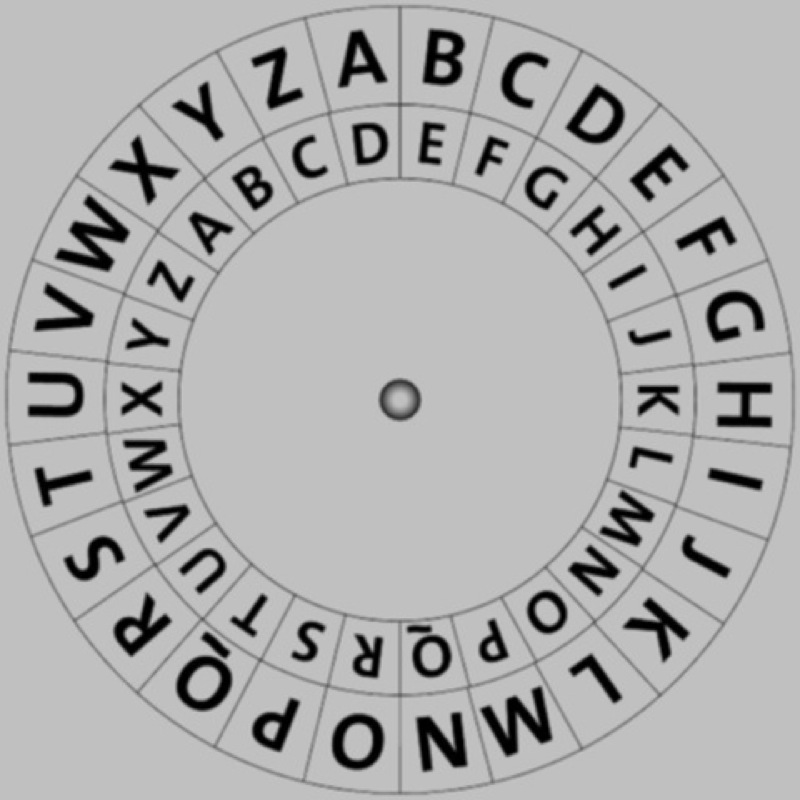
\includegraphics[width=0.382\textwidth]{pictures/caesarscheibe}
\caption{Caesar-Scheibe zum Ver- und Entschlüsseln}
\end{center}
\end{figure}

\subsection{Polyalphabetische Verschlüsselung}

Als eigentlicher Begründer der Kryptologie gilt \textsc{L.B.~Alberti}, der 1466 erstmals den poly\-alpha\-be\-tischen Schlüssel beschrieb. Parallel zur Weiterentwicklung der Kryptologie gab es auch Fortschritte in der Berechnung von Schlüsseln. Um 1400 gelang es den Arabern, Substitutionen zu brechen. \textsc{G.B.~Della Porta} l\"oste erstmals einen polyalphabetischen Schlüssel. Wichtige Beiträge zur Kryptologie lieferten im 19.Jh.~u.a.~\textsc{C.~Wheatstone, F.~Beaufort} und \textsc{Friedrich W.~Kasiski}.

Die polyalphabetische Chiffrierung hat jahrtausendelang seine Bedeutung erhalten und wurde von den Deutschen noch im Zweiten Weltkrieg benutzt. Allerdings wurden dabei nicht Papierstreifen gegeneinander verschoben, sondern eine Maschine verwendet, in der sich Walzen mit eingravierten Buchstaben drehten. Durch Veränderung von Schaltungen, das heisst durch Neustecken von elektrischen Kontakten, konnte man den Code, also die Gr\"osse der einzelnen Verschiebungen, bei der Wahl eines jeden Buchstabens automatisch verändern. Der Empfänger besass eine ähnliche Maschine, \glqq ENIGMA\grqq\ genannt (ENIGMA, griechisch Rätsel, Geheimnis). Da er den jeweils verwendeten Code kannte, konnte er ihn in diese Maschine eingeben und erhielt dann durch Tippen des verschlüsselten Textes unmittelbar die entschlüsselte Botschaft. Auf deutscher Seite war man überzeugt, dass die kriegswichtigen Nachrichten vom Gegner nicht entziffert werden könnten. Man hatte sich aber getäuscht. Zwei Umstände machten es den Polen und Engländern möglich, den Code zu knacken:
\begin{itemize}
\item Weil die Verschlüsselung jeweils nur durch Herstellung von verschiedenen Schaltungen erfolgte, gab es eine endliche Zahl von verschiedenen Codes. Es wurden somit nicht immer wieder neue Codes verwendet, sondern nach einiger Zeit alte nochmals eingesetzt. Durch diese Wiederholung wurden Ansatzpunkte geschaffen, die Verschlüsselung zu knacken.
\item Die Engländer verfügten über die ersten leistungsfähigen elektronischen	Rechenmaschinen (Bomben). Dadurch konnten sie in Sekundenbruchteilen zahlreiche Zu\-ord\-nungs\-m\"og\-lich\-kei\-ten ausprobieren, bis sie durch Zufall auf die richtige stiessen.
\end{itemize}
Den Deutschen blieb verborgen, dass die Engländer ihre Nachrichten verstehen konnten, was nicht unwesentlich zur Entscheidung des Krieges beigetragen haben soll. Zu der Kryptoanalytikergruppe der Engländer geh\"orte unter anderen auch \textsc{A.~Turing}, der nicht unwesentlichen Einfluss auf die Weiterentwicklung der noch jungen Computertechnik hatte. Wesentliche Veränderung für die Kryptologie brachte das Aufkommen des Computers mit sich. Unter dem Aspekt des Datenschutzes hat das Interesse an der Kryptologie ganz erheblich zugenommen. Andererseits bietet der Computer selber die Möglichkeit, grosse Datenmengen schnell analysieren zu k\"onnen, was neue Ansätze zum Brechen von Schlüsseln schafft.

\clearpage

\section{Monoalphabetische Verfahren}

Eine sehr einfache Verschlüsselung erhalten wir, indem wir jedem Buchstaben ein festes Symbol zuordnen. Diese Verfahren heissen \textbf{monoalphabetisch}. Sie sind in der Regel, steht genügend Material zur Verfügung, leicht durch Häufigkeitsbetrachtungen zu berechnen. Wesentlich schwieriger ist es, polyalphabetische Geheimtexte, das sind solche, bei denen einem Buchstaben mehrere Symbole entsprechen k\"onnen, zu brechen, weil hier statistische Erwägungen nicht ohne weiteres angewendet werden k\"onnen. Die klassischen Verfahren haben den Nachteil, dass sich Sender und Empfänger über den zu verwendenden Schlüssel verständigen müssen, was eine zusätzliche Unsicherheit bedeutet. Dies entfällt bei den Public-Key-Systemen, die seit 1976 entwickelt werden. Das bekannteste unter ihnen, das RSA-Verfahren (nach \textsc{R.~Rivest, A.~Shamir} und \textsc{L. Adleman}), verwendet die Primfaktorenzerlegung natürlicher Zahlen. Es ist nur so lange sicher, wie es keine wesentlich schnelleren Algorithmen zur Primfaktorzerlegung gibt als die heute bekannten. Daneben setzt es die Kenntnis genügend vieler grosser Primzahlen voraus.

\begin{wrapfigure}{r}{0.382\textwidth}
\vspace{-22pt}
  \begin{center}
    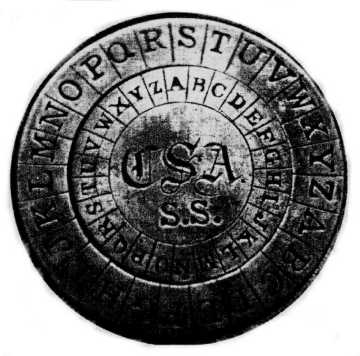
\includegraphics[width=0.3\textwidth]{pictures/Drehsch}
  \end{center}
%\caption{Positive Attitude}
\vspace{-22pt}
\end{wrapfigure}
Monoalphabetische Chiffrierung besteht darin, das Klartextalphabet zu permutieren, d.h. die Buchstabenanordnung wird vertauscht. Unter der Annahme, dass das verwendete Alphabet 26 Buchstaben besitzt (deutsch --- mit ä = ae, ö = oe, ü = ue), erhalten wir also
$$26! = 403291461126605635584000000 \approx 4\cdot10^{26}$$
Mäglichkeiten der Anordnung der Buchstaben.

\subsection{CAESAR-Cipher}
Zu den einfachsten Chiffren gehört die Verschiebechiffre, die schon von \textsc{Caesar} verwendet wurde. Hierbei werden nur die Buchstaben in ihrer Reihenfolge verschoben. Einen solchen Geheimtext k\"onnen wir einfach brechen, da für ein beliebiges Wort nur alle möglichen 26
Verschiebungen betrachtet werden müssen, um ein sinnvolles zu finden. Betrachten wir zum Beispiel \texttt{RBC}, so ergibt nur das Wort \texttt{ist} einen Sinn. Versuchen Sie nun den folgenden berühmten Satz zu dechiffrieren:
\begin{quote}
\texttt{
LFK NDP VDK XQG VLH JWH
}
\end{quote}

\begin{ueb}[Caesar]
Werden
\marginnote{
\qrcode{
https://www.youtube.com/watch?v=asmR0UY42L8}
}
in \texttt{Mathematica} oder \texttt{Python} erledigt.
\end{ueb}

\subsection{Tauschchiffre}

Eine
\marginnote{
\qrcode{
https://www.youtube.com/watch?v=2H1AWu2WfsA}
}
weitere M\"oglichkeit bietet die \textbf{Tauschchiffre}. Hierbei wird nicht einfach das gesamte Alphabet verschoben, sondern die Buchstaben untereinander vertauscht. Mathematisch ausgedrückt heisst das: jedem Buchstabe des Klartextalphabetes wird gemäss der Reihenfolge die entsprechende natürliche Zahl zugeordnet. Multiplizieren wir den Wert eines jeden Klartextbuchstaben mit einer frei wählbaren Zahl, erhalten wir ein neues (im Allgemeinen nicht eindeutiges) Geheimtextalphabet. Soll diese Abbildung eindeutig sein, müssen wir beachten, dass die Geheimzahl und die Anzahl der Klartextbuchstaben zueinander teilerfremd sind. Für ein Alphabet mit 26 Buchstaben sind also nur die Faktoren: $1$, $3$, $5$, $7$, $9$, $11$, $15$, $17$, $19$, $21$, $23$ und $25$ möglich. Wählen wir zum Beispiel $3$ als Faktor, so entsteht das Alphabet in Tabelle \ref{tauschchiffre}

\begin{table}[h!]
\texttt{
\begin{center}
\begin{tabular}{cccccccccccccccccccc}
a&b&c&d&e&f&g&h&i&j&k&l&m&n&o&p&q&r&s&t\\
C&F&I&L&O&R&U&X&A&D&G&J&M&P&S&V&Y&B&E&H\\
u&v&w&x&y&z\\
K&N&Q&T&W&Z
\end{tabular}
\end{center}
}
\normalfont
\caption{Monoalphabetische Verschlüsselung mit Faktor $3$}\label{tauschchiffre}
\end{table}

\begin{ueb}[Tauschchiffre]
Beschreibe die Chiffrierung mathematisch.
\end{ueb}

Natürlich k\"onnen die beiden Verfahren auch miteinander kombiniert werden.

Häufig wird die Methode des Schlüsselwortes verwendet, d.h. Sender und Empfänger vereinbaren ein Schlüsselwort und einen Schlüsselbuchstaben. Dies kann z.B. das fünfte Wort in der Bibel und der zweite Buchstabe des dritten Wortes sein. Somit kann die Chiffrierung jeden Tag mit anderen Voraussetzungen begonnen werden. Zur Vereinfachung wird folgendes angenommen:

\begin{quote}
Schlüsselwort: \texttt{GEHEIMSCHRIFT}	Schlüsselbuchstabe: \texttt{e}
\end{quote}
Zur Chiffrierung werden nun die im Schlüsselwort mehrfach auftretenden Buchstaben bei Wiederholung gestrichen, wir erhalten also
\begin{quote}
\texttt{GEHIMSCRFT}.
\end{quote}

Dann wird der Rest des Schlüsselwortes unter das Klartextalphabet geschrieben, beginnend beim Schlüsselbuchstaben. Es folgt das Auffüllen der restlichen Alphabetbuchstaben.

\begin{table}
\texttt{
\begin{center}
\begin{tabular}{cccccccccccccccccccc}
a&b&c&d&\textcolor{magenta}{e}&f&g&h&i&j&k&l&m&n&o&p&q&r&s&t\\
W&X&Y&Z&\textcolor{red}{G}&\textcolor{red}{E}&\textcolor{red}{H}&\textcolor{red}{I}&\textcolor{red}{M}&\textcolor{red}{S}&\textcolor{red}{C}&\textcolor{red}{R}&\textcolor{red}{F}&\textcolor{red}{T}&A&B&D&J&K&L\\
u&v&w&x&y&z\\
N&O&P&Q&U&V
\end{tabular}
\end{center}
}
\normalfont 
\caption{Monoalphabetische Verschlüsselung mit Schlüssel\-wort und Schlüs\-sel\-buch\-sta\-be}
\end{table}


\subsubsection{Ein praktisches Beispiel}

\label{james}
Wir wollen unserem Verleger die aktuelle Version des neuen Romans schicken. Da der benutzte Weg sehr unsicher ist, soll das Stück verschlüsselt werden. Als Schlüsselwort wurde \texttt{JAMES BOND} vereinbart, der Schlüsselbuchstabe soll das \texttt{q} sein. Wir entfernen zunächst das Leerzeichen aus dem Schlüsselwort und schreiben das Schlüsselwort beginnend beim Buchstaben \texttt{q} auf. Anschliessend ergänzen wir die fehlenden Geheimtextbuchstaben, so dass keiner doppelt vorkommt:

\begin{table}[h!]
\texttt{
\begin{center}
\begin{tabular}{cccccccccccccccccccc}
a&b&c&d&e&f&g&h&i&j&k&l&m&n&o&p&\textcolor{magenta}{q}&r&s&t\\
F&G&H&I&K&L&P&Q&R&T&U&V&W&X&Y&Z&\textcolor{red}{J}&\textcolor{red}{A}&\textcolor{red}{M}&\textcolor{red}{E}\\
u&v&w&x&y&z\\
\textcolor{red}{S}&\textcolor{red}{B}&\textcolor{red}{O}&\textcolor{red}{N}&\textcolor{red}{D}&C
\end{tabular}
\end{center}
}
\normalfont 
\caption{Beispiel einer monoalphabetische Verschlüsselung mit Schlüsselwort \texttt{JAMES BOND} und Schlüsselbuchstabe \texttt{q}}
\end{table}

\noindent Nun wandeln wir schrittweise den Klartext in den Geheimtext um, indem wir für den jeweiligen Klartextbuchstaben den darunter stehenden Geheimtextbuchstaben verwenden.

\begin{quote}
Der abgeschlossene Roman\\
IKA FGPKMHQVYMMKXK AYWFX

Los, hierher ihr beiden!! Wollt ihr wohl hoeren?!\\
VYM, QRKAQKA RQA GKRIKX!! OYVVE RQA OYQV QYKAKX?!\\
Hierher sag' ich! Ja, so ist es brav!\\
QRKAQKA MFP' RHQ! TF, MY RME KM GAFB!\\
So - und jetzt macht ihr schoen Platz!\\
MY - SXI TKECE WFHQE RQA MHQYKX ZVFEC!\\
Na bitte! Und jetzt bei Fuss! Na los!\\
XF GREEK! SXI TKECE GKR LSMM! XF VYM!\\
Bei Fuss hab' ich gesagt!\\
GKR LSMM QFG' RHQ PKMFPT!\\
Fuu\dots  \glqq Mein Gott, Riebesehl\glqq , stoehnt Gatti,\\
LSS\dots  \glqq WKRX PYTT, ARKGKMKQV\glqq , MEYKQXR PFEER,\\
\glqq kannst du nicht einmal deine Socken anziehen\\
\glqq UFXXME IS XRHQE KRXWFV IKRXK MYHUKX FXCRKQKX\\
 wie jeder andere auch??\glqq \\
 ORK TKIKA FXIKAK FSHJ??\glqq
 
 \normalfont 
[aus STERN Hamburg; Heft 29/94 S. 74]

\end{quote}

\subsection{Das Entschlüsseln monoalphabetischer Texte}

Um einen solchen Geheimtext zu entschlüsseln, müssen zwei Bedingungen erfüllt sein. Zum einen muss der Klartext in einer natürlichen Sprache verfasst worden sein, und zum zweiten ein längeres Stück des Geheimtextes vorliegen. Die Analyse des Textes beruht auf der Häufigkeitsverteilung von Buchstaben und Bigrammen in der Sprache. Für Deutsch sieht die Verteilung wie in Tabelle \ref{haeufigkeitDE} auf Seite \pageref{haeufigkeitDE} aus.

\definecolor{Gray}{gray}{0.9}
\definecolor{darkgreen}{rgb}{0,0.4,0}
\definecolor{lightyellow}{rgb}{1,1,0.8}
\arrayrulecolor{darkgreen}
%\doublerulesepcolor{black}

\begin{table}
\begin{center}
\scalebox{0.95}{
\begin{tabular}{|c|c|c|c||c|c|}
\hhline{----||--}
\rowcolor{lightyellow}\spaltenheight \textbf{Buchstabe} &	\textbf{Häufigkeit} &	\textbf{Buchstabe} &	\textbf{Häufigkeit} &	\textbf{Bigramm} &	\textbf{Häufigkeit}\spaltensep
\hhline{----||--}
\rowcolor{Gray}\spaltenheight \texttt{a}&	6.47\% &\texttt{n}&	9.84\%&	\texttt{en}&	3.88\%\spaltensep\hhline{----||--}
\rowcolor{lightyellow}\spaltenheight \texttt{b}&	1.93\% &\texttt{o}	&2.98\%&	\texttt{er}	&3.75\%\spaltensep\hhline{----||--}
\rowcolor{Gray}\spaltenheight \texttt{c}&	2.68\% &\texttt{p}	&0.96\%	&\texttt{ch}	&2.75\%\spaltensep\hhline{----||--}
\rowcolor{lightyellow}\spaltenheight \texttt{d}&	4.83\% &\texttt{q}	&0.02\%	&\texttt{te}	&2.26\%\spaltensep\hhline{----||--}
\rowcolor{Gray}\spaltenheight \texttt{e}&	17.48\% &\texttt{r}&	7.54\%&	\texttt{de}&	2.00\%\spaltensep\hhline{----||--}
\rowcolor{lightyellow}\spaltenheight \texttt{f}&	1.65\%	&\texttt{s}&	6.83\%&	\texttt{nd}	&1.99\%\spaltensep\hhline{----||--}
\rowcolor{Gray}\spaltenheight \texttt{g}&	3.06\%	&\texttt{t}	&6.13\%&	\texttt{ei}	&1.88\%\spaltensep\hhline{----||--}
\rowcolor{lightyellow}\spaltenheight \texttt{h}&	4.23\%	&\texttt{u}	&4.17\%	&\texttt{ie}	&1.79\%\spaltensep\hhline{----||--}
\rowcolor{Gray}\spaltenheight \texttt{i}&	7.73\%	&\texttt{v}	&0.94\%	&\texttt{in}	&1.67\%\spaltensep\hhline{----||--}
\rowcolor{lightyellow}\spaltenheight \texttt{j}&	0.27\%	&\texttt{w}	&1.48\%&	\texttt{es}	&1.52\%\spaltensep\hhline{----||--}
\rowcolor{Gray}\spaltenheight \texttt{k}&	1.46\%	&\texttt{x}	&0.04\%& &\spaltensep\hhline{----||--}
\rowcolor{lightyellow}\spaltenheight \texttt{l}&	3.49\%	&\texttt{y}	&0.08\%& &\spaltensep\hhline{----||--}
\rowcolor{Gray}\spaltenheight \texttt{m}&	2.58\%	&\texttt{z}	&1.14\%& &\spaltensep\hhline{----||--}
\end{tabular}
}
\end{center}
\caption{Relative Deutsche Buchstabenhäufigkeiten von Mono- und Bigrammen}\label{haeufigkeitDE}
\end{table}

Die
\marginnote{
\qrcode{
https://www.youtube.com/watch?v=YonNp_2U2Fc}
}
Vorgehensweise zum Entschlüsseln ist folgende:\\
Man zählt die Häufigkeiten der Buchstaben im Geheimtext und findet so \texttt{e} und \texttt{n} und die Menge $\set{r,i,t,s,a}$. Durch Auszählen der Bigramme kann man dann \texttt{r,i,t,s,a} isolieren und schliesslich über \texttt{ch} noch c und h bestimmen, da das Bigramm \texttt{hc} fast nie vorkommt. Die Buchstaben \texttt{e,n,i,s,r,a,t,c} und \texttt{h} machen bereits rund 65\% des Textes aus. Der Rest ergibt sich durch Probieren.

\subsubsection{Ein weiteres Beispiel}

Gegeben ist folgender monoalphabetisch verfasster Geheimtext:
\begin{quote}
\noindent
\texttt{
FWJNKYICW CAFFL NGXJMHGTK IWLLG FGMTG KYIPMGHGJFNLLGJ PMGZGJ FWR FMHJWGTG FGMTG CWLVGT IWXG MYI HGHGT VRALU GMTHGLWNKYIL ZGTGT HMTH GK KAPMGKA TMYIL XGKATZGJK PWK FWYIL ZGMT INTZ JWNYIL GJ MFFGJ TAYI KA OMGR
\normalfont
}
\end{quote}

\begin{enumerate}
\item Zählen der einzelnen Buchstaben.

\texttt{
\begin{tabular}{ccccccccccccccccc}
A&B&C&D&E&F&G&H&I&J&K&L&M&N&O&P&Q\\
7& 0& 3& 0& 0&11&30& 8&11&10&11&12&14& 6& 1& 4& 0\\
R&S&T&U&V&W&X&Y&Z\\
3&0&15&1&2&11&3&8&5
\end{tabular}
}
\normalfont

Der Buchstabe \texttt{G} tritt am häufigsten auf, deshalb vermuteten wir: \texttt{G}=\texttt{e}.
Da \texttt{n} der zweithäufigste Buchstabe ist, sehen wir, das \texttt{n} entweder \texttt{T} oder \texttt{M} sein muss. Aus der Gleichverteilung der Buchstaben \texttt{s,i,r,a,n,t} folgt, das sie \texttt{T,M,L,F,I,K,J} oder \texttt{W} sind.
$$\texttt{n}\in\set{\texttt{T,M}}$$
$$\set{\texttt{s,i,r,a,t,n}}\subset\set{\texttt{T,M,L,F,I,K,J,W}}$$

\item Zählen der Bigramme, die mit \texttt{e} beginnen, also $\texttt{e}?=\texttt{G}?$.

\texttt{
\begin{tabular}{cccccccc}
GX& GT& GM& GH& GJ& GZ& GL& GK\\
1&6&4&1&6&1&1&3
\end{tabular}
}
\normalfont

Aus der Häufigkeitsverteilung der Bigramme folgt
$$\set{\texttt{en,er}}=\set{\texttt{GT,GJ}}$$ und damit \texttt{n} = \texttt{T} und  \texttt{r} = \texttt{J}.
Wir suchen nun nach \texttt{ei} und \texttt{ie}, da diese mit gleicher Häufigkeit vorkommen.
So finden wir \texttt{i} = \texttt{M}, damit muss aber \texttt{s} = \texttt{K} sein.

\item Zählen der Bigramme, die mit \texttt{e} enden, also ?\texttt{e}=?\texttt{G}.

\texttt{
\begin{tabular}{cccccccccc}
NG& HG& LG& FG& TG& MG& ZG& WG& VG& XG\\
1&5&2&3&4&4&4&1&1&2
\end{tabular}
}
\normalfont

Da \texttt{ie} = \texttt{MG} und \texttt{ne} = \texttt{TG} bereits feststehen, gilt
$$\set{\texttt{te,de}}\subset\set{\texttt{HG,LG,FG,ZG,XG}}$$
Durch Vergleich mit obigen Mengen erhalten wir: $\texttt{t}\in\set{\texttt{L,F}}, \texttt{a}\in\set{\texttt{L,F,I,W}}, \texttt{d}\in\set{\texttt{H,L,F,Z,X}}$

\item Zählen der am häufigsten auftretenden Bigramme.

\texttt{
\begin{tabular}{cccc}
YI& GJ& GT& HG\\
8&6&6&5
\end{tabular}
}
\normalfont

Da \texttt{IY} nicht im Text vorkommt, liegt der Schluss zu \texttt{ch} = \texttt{YI} nah.

\item Aufschreiben der gefundenen Buchstaben.
\texttt{
\begin{quote}
FWJNKYICW CAFFL NGXJMHGTK IWLLG FGMTG KYIPMGHGJFNLLGJ\\
m r sch\phantom{ka}\ \phantom{ko}mmt  \ e\ ri\ ens h\ tte meine sch\ ie\ erm tter\\
PMGZGJ FWR FMHJWGTG FGMTG CWLVGT IWXG MYI HGHGT VRALU\\
\phantom{w}ie\ er m\ l m\ \  r\ ene meine  \phantom{ka}t\ en h\ \ e ich gegen \phantom{zlot}t\ \\
GMTHGLWNKYIL ZGTGT HMTH GK KAPMGKA TMYIL XGKATZGJK PWK\\
einget\ \ scht  \ enen ging es s\ \  ies\  \ \ icht \ es\ n\ ers  \ as\\
FWYIL ZGMT INTZ JWNYIL GJ MFFGJ TAYI KA OMGR\\
m cht  \ ein \ un\ \ r\ \ cht er immer \ \  ch s\   \ \ ie 
\end{quote}
}
\normalfont 
Durch einfache Tests findet man schnell die Buchstaben für \texttt{t} und \texttt{a} sowie: \texttt{t}=\texttt{L}, \texttt{a}=\texttt{W}, \texttt{u}=\texttt{N}, \texttt{w}=\texttt{P}, \texttt{g}=\texttt{H}, \texttt{m}=\texttt{F}, \texttt{b}=\texttt{X}, \texttt{d}=\texttt{Z}, \texttt{o}=\texttt{A}, \texttt{k}=\texttt{Z}, \texttt{l}=\texttt{R}, \texttt{v}=\texttt{O}, \texttt{z}=\texttt{V}, \texttt{y}=\texttt{U}.
 
So heisst der nun geknackte Geheimtext:
\begin{quote}
Maruschka kommt --- †brigens hatte meine Schwiegermutter wieder mal Migräne --- Meine Katzen habe ich gegen Zloty eingetauscht --- denen ging es sowieso nicht besonders --- Was macht Dein Hund? --- Raucht er immer noch so viel?
\end{quote}
\end{enumerate}

\subsection{Hilfsmittel zur Ver- \& Entschlüsselung}

Um Kryptoanalyse betreiben zu k\"onnen, müssen wir uns mit den Gesetzmässigkeiten der Sprache vertraut machen. Solche Normen hat jede Sprache und erstere k\"onnen auch durch geschickte Chiffrierung nicht vollständig beseitigt werden.

\subsubsection{Die Muster einer Sprache}

Muster sind die Art und Weise, wie sich Buchstaben in einem Wort wiederholen. Sie werden über Ziffern ausgedrückt, wobei jeder neue Buchstabe auch eine neue Ziffer erhält, also z.B.:
\begin{center}
\texttt{OTTO} $\longrightarrow$ 1221\\
\texttt{NGRGUUV} $\longrightarrow$ 1232445\\
\texttt{PANAMAKANAL} $\longrightarrow$ 12324252326
\end{center}
Solche Muster bleiben bei der monoalphabetischen Chiffrierung erhalten, d.h. enthält ein Geheimtext keine Muster, so ist er nicht durch monoalphabetischer Chiffrierung entstanden. Muster sind sehr hilfreich bei kurzen Texten.

\subsubsection{Die Abhängigkeit der Häufigkeiten vom Klartext}

Die Angaben über die Einzelbuchstaben schwanken und hängen ausserdem vom Genre des Textes ab. So schreibt Beutelsbacher:

\begin{quote}
\glqq Ein von Zitaten strotzender zoologischer Text über den Einfluss von Ozon auf die Zebras im Zentrum von Zaire wird eine andere Häufigkeitsverteilung aufweisen, als ein Traktat über die amourösen Adventüren des Balthasar Matzbach am Rande des Panamakanals.\grqq
\end{quote}

Häufigkeiten sind um so schärfer, je länger der Text ist.

\subsubsection{Der Wortzwischenraum}

Sicherlich kommen wir auf die Idee, den Wortzwischenraum (Space) mit zu verschlüsseln. Dies führt dann zu einem Alphabet mit 27 Buchstaben. Da der \glqq Space\grqq\ im Deutschen nach dem \texttt{e} das häufigste \glqq Zeichen\grqq\ und somit leicht zu enttarnen ist, lässt der professionelle Chiffrierer diesen Zwischenraum einfach weg, denn dies erschwert die Kryptoanalyse nur unwesentlich.

\subsubsection{Häufigkeiten von n-Grammen}

$n$-Gramme sind Kolonnen von $n$ Buchstaben. Die folgende Tabelle \ref{tab:bigramme} auf Seite \pageref{tab:bigramme} zeigt die Häufigkeiten für Bigramme im Deutschen und Englischen.

\begin{table}
\begin{center}
\begin{tabular}{|c|c||c|c|}
\hhline{--||--}
\rowcolor{lightyellow}\spaltenheight \textbf{Bigramm engl.} &	\textbf{Häufigkeit in \%} &	\textbf{Bigramm dt.} &	\textbf{Häufigkeit in \%}\spaltensep\hhline{--||--}
\rowcolor{Gray}\spaltenheight \texttt{th}&	3.15&	\texttt{en}&	3.88\spaltensep\hhline{--||--}
\rowcolor{lightyellow}\spaltenheight \texttt{he}&	2.51&	\texttt{er}&	3.75\spaltensep\hhline{--||--}
\rowcolor{Gray}\spaltenheight \texttt{an}&	1.72&	\texttt{ch}&	2.75\spaltensep\hhline{--||--}
\rowcolor{lightyellow}\spaltenheight \texttt{in}&	1.69&	\texttt{te}&	2.26\spaltensep\hhline{--||--}
\rowcolor{Gray}\spaltenheight \texttt{er}&	1.54&	\texttt{de}&	2.00\spaltensep\hhline{--||--}
\rowcolor{lightyellow}\spaltenheight \texttt{re}&	1.48&	\texttt{nd}&	1.99\spaltensep\hhline{--||--}
\rowcolor{Gray}\spaltenheight \texttt{on}&	1.45&	\texttt{ei}&	1.88\spaltensep\hhline{--||--}
\rowcolor{lightyellow}\spaltenheight \texttt{es}&	1.45&	\texttt{ie}&	1.79\spaltensep\hhline{--||--}
\rowcolor{Gray}\spaltenheight \texttt{ti}&	1.28&	\texttt{in}&	1.67\spaltensep\hhline{--||--}
\rowcolor{lightyellow}\spaltenheight \texttt{at}&	1.24&	\texttt{es}&	1.52\spaltensep\hhline{--||--}
\end{tabular}
\end{center}
\caption{Bigramm-Häufigkeiten deutsch und englisch}\label{tab:bigramme}
\end{table}

Im Deutschen kommt \texttt{ch} sehr häufig vor, aber nahezu niemals \texttt{hc}. Ferner tauchen \texttt{ei} und \texttt{ie} gleichhäufig auf.

In Tabelle \ref{tab:trigramme} finden Sie noch die Häufigkeit einiger Trigramme.

\begin{table}
\begin{center}
\begin{tabular}{|c|c||c|c|}
\hhline{--||--}
\rowcolor{lightyellow}\spaltenheight \textbf{deutsch} &	\textbf{Häufigkeit in \%} &	\textbf{english} &	\textbf{Häufigkeit in \%}\spaltensep\hhline{--||--}
\rowcolor{Gray}\spaltenheight \texttt{ein}&	1.22&	\texttt{the}&	3.53\spaltensep\hhline{--||--}
\rowcolor{lightyellow}\spaltenheight \texttt{ich}&	1.11&	\texttt{ing}&	1.11\spaltensep\hhline{--||--}
\rowcolor{Gray}\spaltenheight \texttt{nde}&	0.89&	\texttt{and}& 1.02\spaltensep\hhline{--||--}
\rowcolor{lightyellow}\spaltenheight \texttt{die}&	0.87&	\texttt{ion}&	0.75\spaltensep\hhline{--||--}
\rowcolor{Gray}\spaltenheight \texttt{und}&	0.87&	\texttt{tio}&	0.75\spaltensep\hhline{--||--}
\rowcolor{lightyellow}\spaltenheight \texttt{der}&	0.86&	\texttt{ent}&	0.73\spaltensep\hhline{--||--}
\rowcolor{Gray}\spaltenheight \texttt{che}&	0.75&	\texttt{ere}&	0.69\spaltensep\hhline{--||--}
\end{tabular}
\end{center}
\caption{Trigramm-Häufigkeiten deutsch und englisch}\label{tab:trigramme}
\end{table}

Abschliessend eine Aufzählung häufiger Viergramme:
\begin{quote}
deutsch:\q \texttt{icht, keit, heit, chon, chen, cher, urch, eich, \dots}
\end{quote}

Aufschluss über den Ursprung des Textes kann übrigens auch die mittlere Wortlänge geben, oder die $10$ häufigsten Wörter. Betrachten Sie dazu die Tabellen \ref{wortlaenge} und \ref{zehn} auf Seite \pageref{wortlaenge}.

\begin{table}
\begin{center}
\arrayrulecolor{black}
\begin{tabular}{|lc|lc|}
\hline
\rowcolor{Gray}\spaltenheight deutsch&	5.9&	italienisch& 4.5\spaltensep\hline
\rowcolor{lightyellow}\spaltenheight englisch&	4.5&	spanisch& 4.4\spaltensep\hline
\rowcolor{Gray}\spaltenheight französisch& 4.4& russisch& 6.3\spaltensep\hline
\end{tabular}
\end{center}
\caption{Wortlängen von Sprachen}\label{wortlaenge}
\end{table}

\begin{table}
\begin{center}
\begin{tabular}{|l|l|}
\hline
\rowcolor{lightyellow}\spaltenheight \textbf{deutsch} &	\texttt{die, der, und, den, am , in, zu, ist, dass, es}\spaltensep\hline
\rowcolor{Gray}\spaltenheight \textbf{englisch} &	\texttt{the, of, and, to, a, in, that, it, is, I}\spaltensep\hline
\rowcolor{lightyellow}\spaltenheight \textbf{französisch} &	\texttt{de, il, le, et, que, je, la, ne, on, les}\spaltensep\hline
\rowcolor{Gray}\spaltenheight \textbf{italienisch} &	\texttt{la, die, che, il, non, si, le, una, lo, in}\spaltensep\hline
\rowcolor{lightyellow}\spaltenheight \textbf{spanisch} &	 \texttt{de, la, el, que, en, no, con, un, se, sa}\spaltensep\hline
\end{tabular}
\end{center}
\caption{Zehn häufigste Wörter von Sprachen}\label{zehn}
\end{table}

\subsection{Die Abhängigkeit von der Verfassersprache}

\subsubsection{Häufigkeitsgebirge}

Jede Sprache hat ihre eigenen Häufigkeiten. Die Diagrammdarstellungen werden \textbf{Häu\-fig\-keits\-ge\-bir\-ge} genannt. Zwei Beispiele sind in Abbildung \ref{hgebirge} auf Seite \pageref{hgebirge} illustriert.
\begin{figure}
\begin{center}
\definecolor{qqwwqq}{rgb}{0,0.4,0}
\definecolor{zzqqqq}{rgb}{0.6,0,0}
\definecolor{zzzzzz}{rgb}{0.6,0.6,0.6}
\begin{tikzpicture}[line cap=round,line join=round,>=triangle 45,x=0.5cm,y=0.35cm]
\draw [color=zzzzzz,dash pattern=on 2pt off 2pt, xstep=15.0cm,ystep=0.7cm] (0,-0.2) grid (25,19.35);
\draw[-,color=black] (-1.81,0) -- (25.2,0);
\foreach \x in {1,2,3,4,5,6,7,8,9,10,11,12,13,14,15,16,17,18,19,20,21,22,23,24,25}
\draw[shift={(\x,0)},color=black] (0pt,2pt) -- (0pt,-2pt);
\draw[->,color=black] (0,-0.2) -- (0,19.35);
\foreach \y in {2,4,6,8,10,12,14,16,18}
\draw[shift={(0,\y)},color=black] (2pt,0pt) -- (-2pt,0pt) node[left] {\footnotesize $\y$};
%\draw[color=black] (0.15,19) node [anchor=west] { Häufigkeit in \%};
\draw[color=black] (-14pt,5pt) node[right] {\footnotesize $0$};
\clip(-1.81,-2.01) rectangle (27,19.35);
\draw [dash pattern=on 2pt off 2pt,line width=2pt,color=zzqqqq] (17,17)-- (19,17);
\draw[color=black] (19.2,17) node [anchor=west] { deutsch};
\draw [line width=2pt,color=qqwwqq] (17,15)-- (19,15);
\draw[color=black] (19.2,15) node [anchor=west] { englisch};
\draw (0,-0.34) node[anchor=north]{$a$};
\draw (1,-0.1) node[anchor=north]{$b$};
\draw (2,-0.34) node[anchor=north]{$c$};
\draw (3,-0.1) node[anchor=north]{$d$};
\draw (4,-0.34) node[anchor=north] {$e$};
\draw (5,-0.1) node[anchor=north] {$f$};
\draw (6,-0.34) node[anchor=north] {$g$};
\draw (7,-0.1) node[anchor=north] {$h$};
\draw (8,-0.2) node[anchor=north] {$i$};
\draw (9,-0.1) node[anchor=north] {$j$};
\draw (10,-0.1) node[anchor=north] {$k$};
\draw (11,-0.1) node[anchor=north] {$l$};
\draw (12,-0.34) node[anchor=north] {$m$};
\draw (13,-0.34) node[anchor=north] {$n$};
\draw (14,-0.34) node[anchor=north] {$o$};
\draw (15,-0.34) node[anchor=north] {$p$};
\draw (16,-0.34) node[anchor=north] {$q$};
\draw (17,-0.34) node[anchor=north] {$r$};
\draw (18,-0.34) node[anchor=north] {$s$};
\draw (19,-0.2) node[anchor=north] {$t$};
\draw (20,-0.34) node[anchor=north] {$u$};
\draw (21,-0.34) node[anchor=north] {$v$};
\draw (22,-0.34) node[anchor=north] {$w$};
\draw (23,-0.34) node[anchor=north] {$x$};
\draw (24,-0.34) node[anchor=north] {$y$};
\draw (25,-0.34) node[anchor=north] {$z$};
\draw [line width=2pt,color=qqwwqq] (0,8.12)-- (1,1.49);
\draw [line width=2pt,color=qqwwqq] (1,1.49)-- (2,2.78);
\draw [line width=2pt,color=qqwwqq] (2,2.78)-- (3,4.25);
\draw [line width=2pt,color=qqwwqq] (3,4.25)-- (4,12.7);
\draw [line width=2pt,color=qqwwqq] (4,12.7)-- (5,2.23);
\draw [line width=2pt,color=qqwwqq] (5,2.23)-- (6,2.02);
\draw [line width=2pt,color=qqwwqq] (6,2.02)-- (7,6.09);
\draw [line width=2pt,color=qqwwqq] (7,6.09)-- (8,6.97);
\draw [line width=2pt,color=qqwwqq] (8,6.97)-- (9,0.15);
\draw [line width=2pt,color=qqwwqq] (9,0.15)-- (10,0.77);
\draw [line width=2pt,color=qqwwqq] (10,0.77)-- (11,4.03);
\draw [line width=2pt,color=qqwwqq] (11,4.03)-- (12,2.41);
\draw [line width=2pt,color=qqwwqq] (12,2.41)-- (13,6.75);
\draw [line width=2pt,color=qqwwqq] (13,6.75)-- (14,7.51);
\draw [line width=2pt,color=qqwwqq] (14,7.51)-- (15,1.93);
\draw [line width=2pt,color=qqwwqq] (15,1.93)-- (16,0.1);
\draw [line width=2pt,color=qqwwqq] (16,0.1)-- (17,5.99);
\draw [line width=2pt,color=qqwwqq] (17,5.99)-- (18,6.33);
\draw [line width=2pt,color=qqwwqq] (18,6.33)-- (19,9.06);
\draw [line width=2pt,color=qqwwqq] (19,9.06)-- (20,2.76);
\draw [line width=2pt,color=qqwwqq] (20,2.76)-- (21,0.98);
\draw [line width=2pt,color=qqwwqq] (21,0.98)-- (22,2.36);
\draw [line width=2pt,color=qqwwqq] (22,2.36)-- (23,0.15);
\draw [line width=2pt,color=qqwwqq] (23,0.15)-- (24,1.97);
\draw [line width=2pt,color=qqwwqq] (24,1.97)-- (25,0.07);
\draw [dash pattern=on 2pt off 2pt,line width=2pt,color=zzqqqq] (0,6.47)-- (1,1.93);
\draw [dash pattern=on 2pt off 2pt,line width=2pt,color=zzqqqq] (1,1.93)-- (2,2.68);
\draw [dash pattern=on 2pt off 2pt,line width=2pt,color=zzqqqq] (2,2.68)-- (3,4.83);
\draw [dash pattern=on 2pt off 2pt,line width=2pt,color=zzqqqq] (3,4.83)-- (4,17.48);
\draw [dash pattern=on 2pt off 2pt,line width=2pt,color=zzqqqq] (4,17.48)-- (5,1.65);
\draw [dash pattern=on 2pt off 2pt,line width=2pt,color=zzqqqq] (5,1.65)-- (6,3.06);
\draw [dash pattern=on 2pt off 2pt,line width=2pt,color=zzqqqq] (6,3.06)-- (7,4.23);
\draw [dash pattern=on 2pt off 2pt,line width=2pt,color=zzqqqq] (7,4.23)-- (8,7.73);
\draw [dash pattern=on 2pt off 2pt,line width=2pt,color=zzqqqq] (8,7.73)-- (9,0.27);
\draw [dash pattern=on 2pt off 2pt,line width=2pt,color=zzqqqq] (9,0.27)-- (10,1.46);
\draw [dash pattern=on 2pt off 2pt,line width=2pt,color=zzqqqq] (10,1.46)-- (11,3.49);
\draw [dash pattern=on 2pt off 2pt,line width=2pt,color=zzqqqq] (11,3.49)-- (12,2.58);
\draw [dash pattern=on 2pt off 2pt,line width=2pt,color=zzqqqq] (12,2.58)-- (13,9.84);
\draw [dash pattern=on 2pt off 2pt,line width=2pt,color=zzqqqq] (13,9.84)-- (14,2.98);
\draw [dash pattern=on 2pt off 2pt,line width=2pt,color=zzqqqq] (14,2.98)-- (15,0.96);
\draw [dash pattern=on 2pt off 2pt,line width=2pt,color=zzqqqq] (15,0.96)-- (16,0.05);
\draw [dash pattern=on 2pt off 2pt,line width=2pt,color=zzqqqq] (16,0.05)-- (17,7.54);
\draw [dash pattern=on 2pt off 2pt,line width=2pt,color=zzqqqq] (17,7.54)-- (18,6.83);
\draw [dash pattern=on 2pt off 2pt,line width=2pt,color=zzqqqq] (18,6.83)-- (19,6.13);
\draw [dash pattern=on 2pt off 2pt,line width=2pt,color=zzqqqq] (19,6.13)-- (20,4.17);
\draw [dash pattern=on 2pt off 2pt,line width=2pt,color=zzqqqq] (20,4.17)-- (21,0.94);
\draw [dash pattern=on 2pt off 2pt,line width=2pt,color=zzqqqq] (21,0.94)-- (22,1.48);
\draw [dash pattern=on 2pt off 2pt,line width=2pt,color=zzqqqq] (22,1.48)-- (23,0.04);
\draw [dash pattern=on 2pt off 2pt,line width=2pt,color=zzqqqq] (23,0.04)-- (24,0.08);
\draw [dash pattern=on 2pt off 2pt,line width=2pt,color=zzqqqq] (24,0.08)-- (25,1.14);
\fill [color=zzqqqq] (0,6.47) circle (1.5pt);
\fill [color=zzqqqq] (1,1.93) circle (1.5pt);
\fill [color=zzqqqq] (2,2.68) circle (1.5pt);
\fill [color=zzqqqq] (3,4.83) circle (1.5pt);
\fill [color=zzqqqq] (4,17.48) circle (1.5pt);
\fill [color=zzqqqq] (5,1.65) circle (1.5pt);
\fill [color=zzqqqq] (6,3.06) circle (1.5pt);
\fill [color=zzqqqq] (7,4.23) circle (1.5pt);
\fill [color=zzqqqq] (8,7.73) circle (1.5pt);
\fill [color=zzqqqq] (9,0.27) circle (1.5pt);
\fill [color=zzqqqq] (10,1.46) circle (1.5pt);
\fill [color=zzqqqq] (11,3.49) circle (1.5pt);
\fill [color=zzqqqq] (12,2.58) circle (1.5pt);
\fill [color=zzqqqq] (13,9.84) circle (1.5pt);
\fill [color=zzqqqq] (14,2.98) circle (1.5pt);
\fill [color=zzqqqq] (15,0.96) circle (1.5pt);
\fill [color=zzqqqq] (16,0.05) circle (1.5pt);
\fill [color=zzqqqq] (17,7.54) circle (1.5pt);
\fill [color=zzqqqq] (18,6.83) circle (1.5pt);
\fill [color=zzqqqq] (19,6.13) circle (1.5pt);
\fill [color=zzqqqq] (20,4.17) circle (1.5pt);
\fill [color=zzqqqq] (21,0.94) circle (1.5pt);
\fill [color=zzqqqq] (22,1.48) circle (1.5pt);
\fill [color=zzqqqq] (23,0.04) circle (1.5pt);
\fill [color=zzqqqq] (24,0.08) circle (1.5pt);
\fill [color=zzqqqq] (25,1.14) circle (1.5pt);
\fill [color=qqwwqq] (0,8.12) circle (1.5pt);
\fill [color=qqwwqq] (1,1.49) circle (1.5pt);
\fill [color=qqwwqq] (2,2.78) circle (1.5pt);
\fill [color=qqwwqq] (3,4.25) circle (1.5pt);
\fill [color=qqwwqq] (4,12.7) circle (1.5pt);
\fill [color=qqwwqq] (5,2.23) circle (1.5pt);
\fill [color=qqwwqq] (6,2.02) circle (1.5pt);
\fill [color=qqwwqq] (7,6.09) circle (1.5pt);
\fill [color=qqwwqq] (8,6.97) circle (1.5pt);
\fill [color=qqwwqq] (9,0.15) circle (1.5pt);
\fill [color=qqwwqq] (10,0.77) circle (1.5pt);
\fill [color=qqwwqq] (11,4.03) circle (1.5pt);
\fill [color=qqwwqq] (12,2.41) circle (1.5pt);
\fill [color=qqwwqq] (13,6.75) circle (1.5pt);
\fill [color=qqwwqq] (14,7.51) circle (1.5pt);
\fill [color=qqwwqq] (15,1.93) circle (1.5pt);
\fill [color=qqwwqq] (16,0.1) circle (1.5pt);
\fill [color=qqwwqq] (17,5.99) circle (1.5pt);
\fill [color=qqwwqq] (18,6.33) circle (1.5pt);
\fill [color=qqwwqq] (19,9.06) circle (1.5pt);
\fill [color=qqwwqq] (20,2.76) circle (1.5pt);
\fill [color=qqwwqq] (21,0.98) circle (1.5pt);
\fill [color=qqwwqq] (22,2.36) circle (1.5pt);
\fill [color=qqwwqq] (23,0.15) circle (1.5pt);
\fill [color=qqwwqq] (24,1.97) circle (1.5pt);
\fill [color=qqwwqq] (25,0.07) circle (1.5pt);
\end{tikzpicture}
\caption{Häufigkeitsgebirge Deutsch \& Englisch}\label{hgebirge}
\end{center}
\end{figure}
Durch Häufigkeitsgebirge k\"onnen wir bei genügend langem monoalphabetisch chiffriertem Geheimtext feststellen, in welcher Sprache er verfasst wurde.

\subsubsection{Der Koinzidenzindex kappa einer Sprache}

Um das $\kappa$ einer Sprache zu bestimmen, schreiben wir zwei gleichlange unterschiedliche Texte untereinander und zählen alle \glqq Spalten\grqq\ mit gleichen Buchstaben. Anschliessend teilen wir diese Zahl durch die Anzahl der Buchstaben in einer Zeile. Die mathematische Beschreibung von $\kappa$ sieht wie folgt aus.
Für zwei Texte gleicher Länge
$$T_x=x_1x_2\dots x_n\text{ und }T_y=y_1y_2\dots y_n$$
definieren wir
$$\kappa(T_x,T_y)=\sum_{i=1}^n\frac{\gd(x_i,y_i)}{n}\q\text{ wobei }\q\gd(x_i,y_i)=
\begin{cases}
1\q\text{für }x_i=y_i\\
0\q\text{für }x_i\neq y_i
\end{cases}$$
ist. Praktischer ist jedoch die Formel
$$\kappa=\frac{\sum_{i=1}^{26}n_i^2}{n(n-1)},$$
wobei $n$ die Gesamtanzahl der Buchstaben ist und $n_i$ die absolute Häufigkeit der einzelnen Buchstaben.
Es zeigt sich, dass jede Sprache ihr eigenes $\kappa$ hat; siehe dazu Tabelle \ref{tab:sprache} auf Seite \pageref{tab:sprache}.
\begin{table}
\begin{center}
\scalebox{1}{
\begin{tabular}{|lc|lc|}
\hline
\rowcolor{Gray}\spaltenheight deutsch&	7.62\%&	italienisch& 7.38\%\spaltensep\hline
\rowcolor{lightyellow}\spaltenheight englisch&	6.61\%&	spanisch& 7.75\%\spaltensep\hline
\rowcolor{Gray}\spaltenheight französisch& 7.78\%& russisch& 5.29\%\spaltensep\hline
\rowcolor{lightyellow}\spaltenheight japanisch& 8.19\%& & \spaltensep\hline
\end{tabular}
}
\end{center}
\caption{Koinzidenzindex $\kappa$ von Sprachen}\label{tab:sprache}
\end{table}
\begin{bem}
Kommt jeder Buchstabe (bei einem Alphabet von $26$ Buchstaben) mit der gleichen Wahrscheinlichkeit von $\frac{1}{26}$ vor, so ergibt sich
$$\kappa=\frac{1}{26}\approx3.85\%$$
\end{bem}
Durch Zerschneiden des Geheimtextes in zwei Hälften und der Ermittlung des $\kappa$ der beiden so entstandenen Texte kann festgestellt werden, mit welcher Sprache der Klartext verfasst wurde; oder ob es sich um eine Kunstsprache handelt.

Gegeben ist folgender monoalphabetischer Text. Versuche diese Nachricht zu knacken!

\begin{quote}
\texttt{
IU MGF IWH UVHHWKIF DVFKIH. RWI SGOHIWRITAUI AGYYI IU UWTA GOC IWHID UYIWH KISOIYXWTA KIDGTAY. EXVIYSXWTA NGD RIF COTAU GOU RID MGXR KIFGHHY. IF UYOIFSI GOC RWI ITAUI SO. RG NGD RWI NFIOSVYYIF ZVD KGOD OHR CWIX GOC RIH COTAU UWI UGA WAH GH OHR VICCHIYI WAFIH DOHR. GXU RIF COTAU RWI UEWYSIH KWCYSGIAHI UGA, FGHHYI IF UV UTAHIXX IF NVHHYI RGZVH. OHR MIHH IF HWTAY KIUYVFKIH UV FIHHY IF HVTA AIOYI.}
\end{quote}
\normalfont

\begin{bem}
Nach Bauer gilt:
\begin{quote}
Ein ideal für die Chiffrierung vorbereiteter Klartext ist orthographisch falsch, sprachlich knapp und stilistisch grauenhaft.
\end{quote}
\end{bem}

\textbf{Polyalphabetische Chiffrierung} bedeutet, dass das Prinzip der monoalphabetischen Chiffrierung nach gewissen Regeln ständig verändert wird. Es wird nicht der gesamte Klartext monoalphabetisch, sondern jede Buchstabengruppe mit einem anderen monoalphabetischen Schlüssel chiffriert.

\clearpage

\section{Die Idee der polyalphabetischen Chiffrierung}
\begin{wrapfigure}{r}{0.382\textwidth}
\vspace{-22pt}
  \begin{center}
    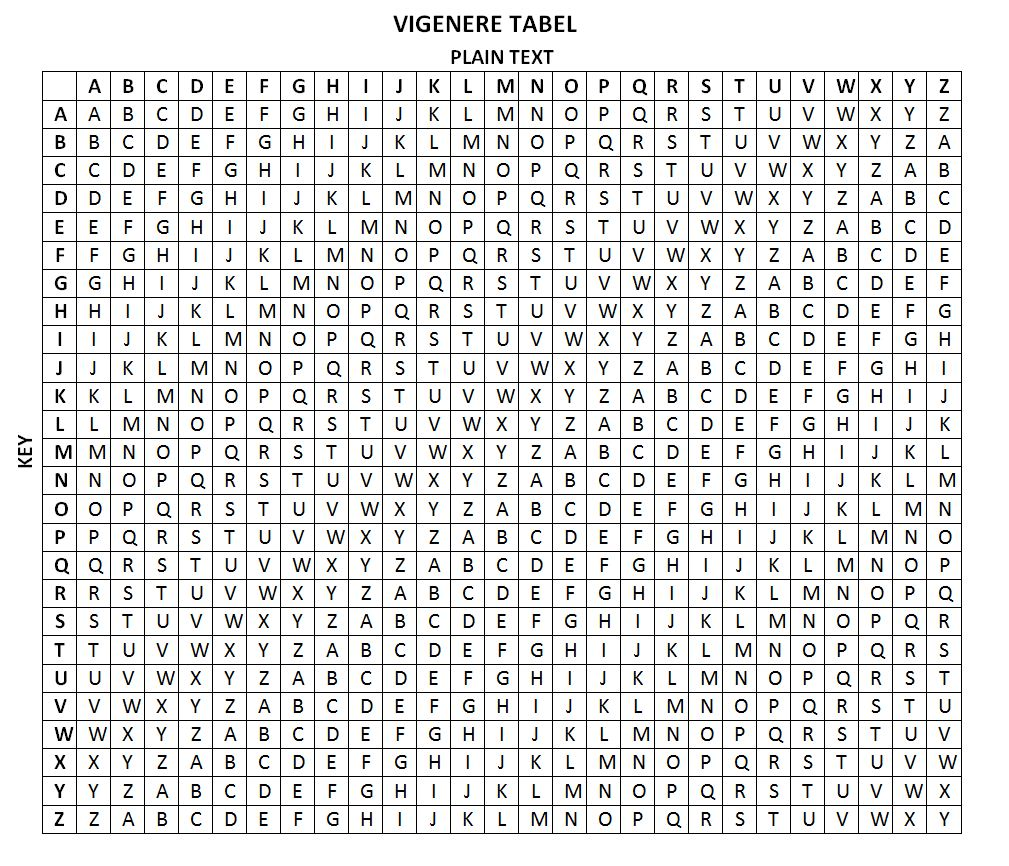
\includegraphics[width=0.29\textwidth]{pictures/vigeneretable}
  \end{center}
%\caption{Positive Attitude}
\vspace{-22pt}
\end{wrapfigure}
Eine polyalphabetische Chiffrierung kann z.B. für den Klartext \texttt{abba} so wie in Tabelle \ref{polyalph} auf Seite \pageref{polyalph} erfolgen.
\begin{table}
\begin{tabular}{lcccccl}
\spaltenheight Klartextalphabet & \texttt{a}& \texttt{b}& \texttt{c}& \texttt{d}& \texttt{e}& \dots\spaltensep
\spaltenheight erstes Geheimtextalphabet & \textcolor{blue}{\texttt{H}}& \texttt{L}& \texttt{W}& \texttt{X}& \texttt{D}& \dots\spaltensep
\spaltenheight zweites Geheimtextalphabet & \texttt{U}& \textcolor{blue}{\texttt{L}}& \texttt{V}& \texttt{W}& \texttt{A}& \dots\spaltensep
\spaltenheight drittes Geheimtextalphabet & \texttt{N}& \textcolor{blue}{\texttt{A}}& \texttt{R}& \texttt{T}& \texttt{I}& \dots\spaltensep
\spaltenheight viertes Geheimtextalphabet & \textcolor{blue}{\texttt{D}}& \texttt{Y}& \texttt{Z}& \texttt{L}& \texttt{M}& \dots\spaltensep
\end{tabular}
\caption{Polyalphabetische Chiffrierung}\label{polyalph}
\end{table}
Damit wird aus \texttt{abba} ganz einfach \texttt{HLAD}. Als Konsequenz ergibt sich, dass die Häufigkeiten und Muster verschwunden sind! Allerdings müssen Empfänger und Sender die Regeln wissen, nachdem sich die Zuordnung Klartextalphabet zu Geheimtextalphabet ändert, im allgemeinen besitzen beide 26 Alphabete und müssen dazu das Anfangswort über\-mit\-teln. Die bekannteste Methode der polyalphabetischen Chiffrierung ist die \textbf{Vigen\`ere-Chiffrierung}. Dazu benötigt man ein sogennantes \textbf{Vigen\`ere-Quadrat}.

\subsection{Vigen\`ere-Chiffrierung}

Neben
\marginnote{
\qrcode{
https://www.youtube.com/watch?v=zZhLLYdDnIQ}
}
dem Vigen\`ere-Quadrat benötigen wir noch ein Schlüsselwort. Um Klartext zu chiffrieren, schreibt man das Schlüsselwort, hier \texttt{VENUS}, periodisch über den Klartext.
\begin{table}
\texttt{
\begin{center}
\begin{tabular}{cccccccccccccccc}
\spaltenheight  V & E& N& U& S& V& E& N& U& S& V& E& N& U& S& V\spaltensep
\spaltenheight  p & o& l& y& a& l& p& h& a& b& e& t& i& s& c& h\spaltensep
\spaltenheight  K & S& Y& S& S& G& T& U& U& T& Z& X& V& M& U& C\spaltensep
\end{tabular}
\end{center}
}
\normalfont
\caption{Vigen\`ere-Chiffrierung}
\end{table}

\noindent Jeder Klartextbuchstabe wird dann mit dem Geheimtextalphabet verschlüsselt, dessen erster Buchstabe im Vigen\`ere-Quadrat über dem Klartextbuchstabe stehende Schlüs\-sel\-wort\-buch\-sta\-be ist. Also für den ersten Buchstaben des Beispiels von oben heisst das: Wenn man das erste \texttt{p} aus polyalphabetisch verschlüsselt will, muss man die Geheimtextalphabetzeile nehmen, die mit \texttt{V} beginnt. Dann sucht man sich im Klartextalphabet über den Vigen\`ere-Quadrat das \texttt{p}, geht die Spalte nach unten bis auf die Höhe von \texttt{V}. Der Geheimtextbuchstaben ist \texttt{K}. Die Dechiffrierung erfolgt analog.

\subsection{Ein praktisches Beispiel}

Dazu verwenden wir den Text, den abgeschlossenen Roman; das Schlüsselwort sei \texttt{JAMES\-BOND}. Wir schreiben zunächst das Schlüsselwort über den Text.
Wir gehen in die Zeile, die mit dem Schlüsselwortbuchstaben beginnt und suchen die Spalte, die mit dem Klartextbuchstaben beginnt. Am Schnittpunkt von Zeile und Spalte steht unser Geheimbuchstabe.
\begin{table}
\texttt{\small
\begin{center}
\scalebox{1.0}{
\begin{tabular}{ccc>{\columncolor{lightyellow}}ccccccccccccccccc}
\spaltenheight a&b&c&\textcolor{blue}{d}&e&f&g&h&i&j&k&l&m&n&o&p&q&r&\dots  \spaltensep
\spaltenheight A&B&C&D&E&F&G&H&I&J&K&L&M&N&O&P&Q&R&\dots  \spaltensep
\spaltenheight B&C&D&E&F&G&H&I&J&K&L&M&N&O&P&Q&R&S&\dots  \spaltensep
\spaltenheight C&D&E&F&G&H&I&J&K&L&M&N&O&P&Q&R&S&T&\dots  \spaltensep
\spaltenheight D&E&F&G&H&I&J&K&L&M&N&O&P&Q&R&S&T&U&\dots  \spaltensep
\spaltenheight E&F&G&H&I&J&K&L&M&N&O&P&Q&R&S&T&U&V&\dots  \spaltensep
\spaltenheight F&G&H&I&J&K&L&M&N&O&P&Q&R&S&T&U&V&W&\dots  \spaltensep
\spaltenheight G&H&I&J&K&L&M&N&O&P&Q&R&S&T&U&V&W&X&\dots  \spaltensep
\spaltenheight H&I&J&K&L&M&N&O&P&Q&R&S&T&U&V&W&X&Y&\dots  \spaltensep
\spaltenheight I&J&K&L&M&N&O&P&Q&R&S&T&U&V&W&X&Y&Z&\dots  \spaltensep
\rowcolor{lightyellow}\spaltenheight \textcolor{red}{J}&K&L&\textcolor{cyan}{M}&N&O&P&Q&R&S&T&U&V&W&X&Y&Z&A&\dots  \spaltensep
\spaltenheight K&L&M&N&O&P&Q&R&S&T&U&V&W&X&Y&Z&A&B&\dots  \spaltensep
\spaltenheight L&M&N&O&P&Q&R&S&T&U&V&W&X&Y&Z&A&B&C&\dots  \spaltensep
\spaltenheight &&&&&&&\multicolumn{5}{c}{\dots\ \dots\ \dots}&&&&&&
\end{tabular}
}
\end{center}
}
\normalfont\normalsize
\caption{Vigen\`ere-Verschlüsselung}
\end{table}
Wir erhalten somit den in Tabelle \ref{tab:james} dargestellten Geheimtext.
\begin{table}
\begin{center}
\texttt{
\begin{tabular}{ccccccccc}
JAMES & & BONDJ & & AMESB & & ONDJA & & ME \spaltensep
Derab & & gesch & & losse & & neRom & & an \spaltensep
MEDET & & HSFFQ & & LAWKF & & BRUXM & & MR
\end{tabular}
}
\caption{Vigen\`ere-Verschlüsselung mit \texttt{JAMESBOND}}\label{tab:james}
\end{center}
\end{table}
\begin{ueb}[Vigen\`ere]
Die Verschlüsselung des restlichen Textes ist eine mögliche Übungsaufgabe.
\end{ueb}

\subsection{Die Theorie der Entschlüsselung}

Die Kryptoanalyse von Vigen\`ere-Chiffrierung ist leicht, wenn das Schlüsselwort relativ kurz ist und der Geheimtext lang. Das Knacken erfolgt in zwei Schritten:
\begin{enumerate}
\item Bestimmen der Länge des Schlüsseltextes (Kasiski- \&\ Friedmann-Test).
\item Bestimmen des Schlüsselwortes selbst.
\end{enumerate}

\subsubsection{Der Kasiski-Test}

Der Test basiert auf folgender Idee:
Treten im Klartext gewisse Buchstabenfolgen häufig auf (Trigramme u.ä.), so werden sie stets gleich übersetzt, wenn ein Vielfaches des Schlüsselwortes dazwischen passt.
\begin{table}
\begin{tabular}{cccccccccccccccccccc}
\spaltenheight V& E& N& U& S& V& E& N& U& S& V& E& N& U& S& V& E& N& U& S \spaltensep
\spaltenheight & & & & e& i& n& & & & e& i& n& & e& i& n& & &\spaltensep
\spaltenheight & & & & \textbf{\texttt{ W}}& \textbf{\texttt{ D}}& \textbf{\texttt{ R}}& & & & Z& M& A& & \textbf{\texttt{ W}}& \textbf{\texttt{ D}}& \textbf{\texttt{ R}}& & &\spaltensep
\end{tabular}
\caption{Idee Kasiski-Test}
\end{table}
Man sucht im Geheimtext sich wiederholende Zeichenfolgen und vermutet, dass
deren Abstand ein Vielfaches der Schlüsselwortlänge ist.

\begin{bsp}
Wir finden sogar Zehngramme:
\definecolor{darkgreen}{rgb}{0,0.5,0}
\texttt{
\begin{quote}
UEQPC VC\textcolor{red}{KAH}  VNRZU  RNLAO  KIRVG  \textcolor{blue}{JTD}VR  VRICV  IDLMY\\
IYSBC  COJQS ZNYMB  VDLOK  FSLMW  EFRZA  \textcolor{cyan}{VIQM}F  \textcolor{blue}{JTD}IH\\
CIFPS  EBXMF  F\textcolor{darkgreen}{TDMH  ZGNMW K}AXAU  VUHJH  NUULS  VSJIP\\
JCKTI VSVMZ  JENZS  \textcolor{red}{KAH}ZS  UIHQV  IBXMF  FIPLC  XEQXO\\
CAVBV RTWMB LNGNI VRLPF V\textcolor{darkgreen}{TDMH ZGNMW K}RXVR QEKVR\\
LKDBS EIPUC EAWJS BAPMB VSZCF UEGIT LEUOS JOUOH\\
UAVAG ZEZIS YRHVR ZHUMF RRE\textcolor{darkgreen}{MW K}ULKV KGHAH FEUBK\\
LRGMB JIHLI IFWMB ZHUMP LEUWG RBHZO LCKCW THWDS\\
ILDAG VNEMJ FRVQS \textcolor{cyan}{VIQM}U VSWMZ CTHII WGDJS XEOWS\\
JTKIH KEQ
\end{quote}
}
\normalfont

\begin{table}
\begin{center}
\scalebox{0.8}{
\begin{tabular}{|lcl|}
\hhline{---}
\rowcolor{lightyellow}\spaltenheight \textbf{Folge} &	\textbf{Abstand} &	\textbf{Primfaktorzerlegung} \spaltensep\hhline{---}
\rowcolor{Gray}\spaltenheight \texttt{KAH}&	128&	$2^7$\spaltensep\hhline{---}
\rowcolor{lightyellow}\spaltenheight \texttt{JTD}&	50&	$2\cdot5^2$\spaltensep\hhline{---}
\rowcolor{Gray}\spaltenheight \texttt{VIQM}&	265&	$3\cdot5^2$\spaltensep\hhline{---}
\rowcolor{lightyellow}\spaltenheight \texttt{TDMHZGNMWK}&	90&	$2\cdot3^2\cdot5$\spaltensep\hhline{---}
\rowcolor{Gray}\spaltenheight \texttt{MWK}&	75&	$3\cdot5^2$\spaltensep\hhline{---}
\end{tabular}
}
\caption{Kasiski-Test}\label{kasiski}
\end{center}
\end{table}
Man bildet nun den grössten gemeinsamen Teiler der Abstandszahlen (siehe Tabelle \ref{kasiski}). In obigen Beispiel wäre dieser $\ggT = 1$, d.h. die Schlüsselwortlänge eins. Dies scheidet aber aus, weil der Klartext dann monoalphabetisch verschlüsselt sein müsste. Nimmt man aber an, dass \texttt{KAH} nur zufällig mehrmals auftritt, dann ist der $\ggT$ der Abstände gleich $5$. Das legt die Schlüsselwortlänge fünf nahe. Es könnte aber auch sein, dass sich \texttt{VIQM} und \texttt{MWK} zufällig wiederholen, dann wäre $\ggT(50, 90) = 10$. Also: die Schlüsselwortlänge ist höchstwahrscheinlich fünf, könnte aber auch zehn sein.
\end{bsp}

\subsubsection{Der Friedmann-Test}

Die Idee des Friedmanntests ist folgende: Je länger das Schlüsselwort ist, desto regelmässiger sind die Häufigkeiten verteilt, desto kleiner bzw. näher liegt $\kappa_G$ an $3,85\%$.
Man nimmt nun an, die Schlüsselwortlänge sei $n$ und schreibt den Geheimtext in $n$ Spalten. Das sieht dann wie folgt aus:
$$
\begin{matrix}
S_{1\phantom{x+1}} & S_{2\phantom{x+1}} & \dots & S_{n\phantom{1}}\\
B_{n+1\phantom{1}} & B_{n+2\phantom{1}} & \dots & B_{2n}\\
B_{2n+1} & B_{2n+2} & \dots & B_{3n}\\
B_{3n+1} & B_{3n+2} & \dots & B_{4n}\\
\vdots & \vdots & \vdots & \vdots
\end{matrix}
$$
Die Wahrscheinlichkeit, dass zwei beliebige Buchstaben in der gleichen Spalte stehen ist
$$\frac{1}{n}\cdot\frac{1}{n}+\frac{1}{n}\cdot\frac{1}{n}+\dots+\frac{1}{n}\cdot\frac{1}{n}=n\cdot\frac{1}{n}\cdot\frac{1}{n}=\frac{1}{n}$$
Die Wahrscheinlichkeit, dass zwei beliebige Buchstaben in unterschiedlichen Spalten stehen, ist dann $1-\frac{1}{n}$.
Die Wahrscheinlichkeit, das zwei beliebige Buchstaben in einer Spalte gleich sind, ist $\kappa_K$ (Klartextkappa); die Buchstaben einer Spalte sind ja dann monoalphabetisch verschlüsselt.
Die Wahrscheinlichkeit, dass zwei Buchstaben aus verschiedenen Spalten gleich sind, ist $3,85\%+\ge$, da über verschiedene Alphabete verschlüsselt wurde. Die Wahrscheinlichkeit, dass zwei beliebige Buchstaben des Geheimtextes gleich sind, ist dann
$$\kappa_G=\frac{1}{n}\kappa_K+(1-\frac{1}{n})\cdot(3.85\%+\ge)=\frac{1}{n}(\kappa_K-3.85\%-\ge)+3.85\%+\ge$$
Da $\kappa_K$ und $\kappa_G$ leicht bestimmt werden k\"onnen, lässt sich die Schlüsselwortlänge bestimmen, indem man nach $n$ auflöst.
$$n=\frac{\kappa_K-3.85\%-\ge}{\kappa_G-3.85\%-\ge}$$
Für deutsch ist $\kappa_K=7.62$ und daher in Prozenten
$$n=\frac{7.62-3.85-\ge}{\kappa_G-3.85-\ge}=\frac{3.77-\ge}{\kappa_G-3.85-\ge}\leq\frac{3.77}{\kappa_G-3.85}$$
Im oben aufgeführten Beispiel ist $\kappa_G=4.39$, woraus $n\leq6.98$ folgt.
Kasiski- und Friedmann-Test legen also die Schlüsselwortlänge $n=5$ nahe.

\subsubsection{Die Bestimmung des Schlüsselwortes}

Da die Schlüsselwortlänge nun bekannt ist, kann das Schlüsselwort einfach gefunden werden. Ist die Länge des Schlüsselwortes gleich $n$, schreibt man den Text wie folgt:
$$
\begin{matrix}
S_{1\phantom{x+1}} & S_{2\phantom{x+1}} & \dots & S_{n\phantom{1}}\\
B_{n+1\phantom{1}} & B_{n+2\phantom{1}} & \dots & B_{2n}\\
B_{2n+1} & B_{2n+2} & \dots & B_{3n}\\
B_{3n+1} & B_{3n+2} & \dots & B_{4n}\\
\vdots & \vdots & \vdots & \vdots
\end{matrix}
$$
Jede
\marginnote{
\qrcode{
https://www.youtube.com/watch?v=lLlc57Kk2Os}
}
Spalte wurde monoalphabetisch verschlüsselt. Es genügt also, das \texttt{e} zu finden, um herauszukriegen mit welchem Alphabet die entsprechende Spalte verschlüsselt wurde. Man entnimmt diese \texttt{e}s der Tabelle.\\
\begin{table}[h!]
\begin{center}
\scalebox{0.8}{
\begin{tabular}{|ccc|}
\hhline{---}
\rowcolor{lightyellow}\spaltenheight \textbf{Spalte} &	\textbf{häufigster Buchstabe} &	\textbf{Schlüsselwortbuchstabe} \spaltensep\hhline{---}
\rowcolor{Gray}\spaltenheight 1&	\texttt{V}$\longrightarrow$\texttt{e}&	\texttt{R}\spaltensep\hhline{---}
\rowcolor{lightyellow}\spaltenheight 2&	\texttt{E}$\longrightarrow$\texttt{e}&	\texttt{A}\spaltensep\hhline{---}
\rowcolor{Gray}\spaltenheight 3&	\texttt{H,D,U}$\longrightarrow$\texttt{e}&	\texttt{D,Z,Q}\spaltensep\hhline{---}
\rowcolor{lightyellow}\spaltenheight 4&	\texttt{N}$\longrightarrow$\texttt{e}&	\texttt{I}\spaltensep\hhline{---}
\rowcolor{Gray}\spaltenheight 5&	\texttt{S}$\longrightarrow$\texttt{e}&	\texttt{O}\spaltensep\hhline{---}
\end{tabular}
}
\end{center}
\end{table}
Das Schlüsselwort lautet also \texttt{RADIO}. Nun kann der gesamte Geheimtext dechiffriert werden.

\subsection{Ein weiteres Beispiel}

Gegeben sei folgender Text:
\texttt{
\begin{quote}
KWCSS  GXYUT  ZBZMU  CMRFY  JZZNZ  HMEBS  WMEXA  ZMZAW\\
IATBS  ABUUK  NMZHT  ZAKCE  HBVLY  ZPVCE  OMONT  PKYML\\
VJVGW  CZRFK  ZQEYF  FTRLL  ZFKVM  XPJNS  WMEXS  MAKYD\\
GMEES  IVRVW  MURHV  VZWHA  XPKPW  MOVMK  ZVUUK  NLVLY\\
ZPVCE  OMONV  ZVBFS  MBVRL  ZQEXW  PBZAT  ZAKCE  HMEGM\\
NAQOE  WMZMH  DMCCK  OMJHA  XPKGG  ZOICU  CLRMK  DMVCF\\
ZURFY  JZZNZ  HCJXW  MOVBW  DUKYP  OJLWZ  NBRVW  IQDED\\
VZKYP  OMZHE  VTVOF  YMZHS  ILVLW  NURFK  ZVKMH  MQTBL\\
JPEYV  VAJYK  YIWOW  MMZHW  MMXYD  BQSNV  DMUYE  ZUGZS\\
ZVXYJ  BMEUM  NIXNO  VVEYJ  ZCEXO  VVEYJ  NMENK  KZZWZ\\
OMJCK  OMENK  XPVCV  ZVUXS  NARHB  ZLVLK  OMCFW  YMJEJ\\
TXKIY  MIDGK  YMIMU  CTLYK  NMCYA  ILVOL  DOUYF  FTRLL\\
ZFKVM  XPJNS  WMETM  EMUYE  BMYYA  HBVRL  WCTBK  OISYF\\
AMJND  ZOK
\end{quote}
}
\normalfont
Wir führen zunächst den Kasiski-Test durch. Dazu suchen wir im Text nach gleichen Textfolgen:
\texttt{
\begin{quote}
KWCSS  GXYUT  ZBZMU  CMRFY  JZZNZ  HMEB\underline{S  WMEX}A  ZMZAW\\
IATBS  AB\textcolor{cyan}{UUK}  NMZHT  ZAKCE  HBVLY  ZPVCE  \textcolor{red}{OMO}NT  PKYML\\
VJVGW  CZRFK  ZQE\textcolor{blue}{YF  FTRLL  ZFKVM  XPJN\underline{S  WME}}\underline{X}S  MAKYD\\
GMEES  IVRVW  MURHV  VZWHA  XPKPW  MOVMK  \underline{ZV}\textcolor{cyan}{\underline{U}UK}  NLVLY\\
ZPVCE  \textcolor{red}{OMO}NV  ZVBFS  MBVRL  ZQEXW  PBZAT  ZAKCE  HMEGM\\
NAQOE  WMZMH  DMCCK  OMJHA  XPKGG  ZOICU  CLRMK  DMVCF\\
ZURFY  JZZNZ  HCJXW  MOVBW  DUKYP  OJLWZ  NBRVW  IQDED\\
VZKYP  OMZHE  VTVOF  YMZHS  ILVLW  NURFK  ZVKMH  MQTBL\\
JPEYV  VAJYK  YIWOW  MMZHW  MMXYD  BQSNV  DMUYE  ZUGZS\\
ZVXYJ  BMEUM  NIXNO  VVEYJ  ZCEXO  VVEYJ  NMENK  KZZWZ\\
OMJCK  OMENK  XPVCV  \underline{ZVU}XS  NARHB  ZLVLK  OMCFW  YMJEJ\\
TXKIY  MIDGK  YMIMU  CTLYK  NMCYA  ILVOL  DOU\textcolor{blue}{YF  FTRLL\\
ZFKVM  XPJNS  WME}TM  EMUYE  BMYYA  HBVRL  WCTBK  OISYF\\
AMJND  ZOK
\end{quote}
}
\normalfont
\begin{table}[h!]
\begin{center}
\scalebox{0.8}{
\begin{tabular}{|lcl|}
\hhline{---}
\rowcolor{lightyellow}\spaltenheight \textbf{Folge} &	\textbf{Abstand} &	\textbf{Primfaktorzerlegung} \spaltensep\hhline{---}
\rowcolor{Gray}\spaltenheight \texttt{SWMEX}&	80&	$2^2\cdot5$\spaltensep\hhline{---}
\rowcolor{lightyellow}\spaltenheight \texttt{UUK}&	105&	$3\cdot5\cdot7$\spaltensep\hhline{---}
\rowcolor{Gray}\spaltenheight \texttt{OMO}&	95&	$5\cdot19$\spaltensep\hhline{---}
\rowcolor{lightyellow}\spaltenheight \texttt{YFFTRLLZFKVMXPJNSWME}&	380&	$2^2\cdot5\cdot19$\spaltensep\hhline{---}
\rowcolor{Gray}\spaltenheight \texttt{ZVU}&	265&	$5\cdot53$\spaltensep\hhline{---}
\end{tabular}
}
\end{center}
\end{table}
Wir bilden nun den grössten gemeinsamen Teiler der Abstandszahlen. Dieser $\ggT$ ist $5$, d.h. die Schlüsselwortlänge hat vermutlich die Länge fünf.

Wir führen jetzt den Friedmann-Test durch. Dazu bestimmen wir die Anzahl der Buchstaben und ihre absolute Häufigkeit. In unserem Fall ist $n = 528$ und
\begin{table}[h!]
\texttt{
\begin{tabular}{ccccccccccccccccc}
A&B&C&D&E&F&G&H&I&J&K&L&M&N&O&P&Q\\
16& 17& 20& 11& 27&15&8& 15&12&17&30&21&51& 20& 22& 13& 6\\
R&S&T&U&V&W&X&Y&Z\\
13&14&18&39&22&16&29&43
\end{tabular}
}
\normalfont
\end{table}
Damit k\"onnen wir die Formel
$$\kappa=\frac{\sum_{i=1}^{26}n_i^2}{n(n-1)}$$
anwenden und erhalten
$$\kappa=\frac{13644}{528\cdot527}=4.9\%.$$
Nun ist es möglich, die Schlüsselwortlänge zu bestimmen:
$$l\approx\frac{3.77}{4.9-3.85}\approx3.6.$$
Wir vermuten also eine Schlüsselwortlänge von drei.
Der Vergleich der beiden Methoden zeigt, dass kein eindeutiges Resultat entsteht. Wir probieren zunächst die Vermutung der Schlüsselwortlänge fünf, da der Kasiski-Test eindeutig funktionierte. Dazu schreiben wir den Text in Spalten zu je fünf Zeichen.
\texttt{
\begin{quote}
KWCSS \dots\\
GXYUT \dots\\
ZBZMU \dots\\
CMRFY \dots\\
JZZNZ \dots
\end{quote}
}
\normalfont
Wir suchen nun in jeder Spalte den häufigsten Buchstaben und nehmen an, dass dieser für \texttt{e} steht.
\begin{table}[h!]
\begin{center}
\scalebox{0.8}{
\begin{tabular}{|ccc|}
\hhline{---}
\rowcolor{lightyellow}\spaltenheight \textbf{Spalte} &	\textbf{häufigster Buchstabe} &	\textbf{Schlüsselwortbuchstabe} \spaltensep\hhline{---}
\rowcolor{Gray}\spaltenheight 1&	\texttt{Z}$\longrightarrow$\texttt{e}&	\texttt{V}\spaltensep\hhline{---}
\rowcolor{lightyellow}\spaltenheight 2&	\texttt{M}$\longrightarrow$\texttt{e}&	\texttt{I}\spaltensep\hhline{---}
\rowcolor{Gray}\spaltenheight 3&	\texttt{V}$\longrightarrow$\texttt{e}&	\texttt{R}\spaltensep\hhline{---}
\rowcolor{lightyellow}\spaltenheight 4&	\texttt{Y}$\longrightarrow$\texttt{e}&	\texttt{U}\spaltensep\hhline{---}
\rowcolor{Gray}\spaltenheight 5&	\texttt{W,K}$\longrightarrow$\texttt{e}& \texttt{S,G}\spaltensep\hhline{---}
\end{tabular}
}
\end{center}
\end{table}
Wie unschwer zu sehen ist, lautet das Schlüsselwort vermutlich \texttt{VIRUS}. Wir k\"onnen den restlichen Text dechiffrieren.

Wir entschlüsseln und erhalten als Resultat:
\begin{quote}
Polyalphabetische Algorithmen haben die Eigenschaft, dass ein bestimmter Geheimtextbuchstabe mehr als einen Klartextbuchstaben darstellen kann. Aber man darf nicht vergessen, dass der Geheimtext den Klartext eindeutig bestimmen muss. Zum Beispiel ist es nicht moeglich, das sie einem Algorithmus der Geheimtextbuchstaben im Klartext einmal \texttt{e} und ein anderes mal \texttt{s} entspricht, ohne dass es dafuer eine Regel gibt, die dem Empfaenger genau sagt, wann er \texttt{e} und wann er \texttt{s} entspricht. Es ist entscheidend, dass an jeder Stelle des Kryptogramms der Schluessel eindeutig den Klartextbuchstaben	zu jedem Geheimtextbuchstaben festlegt.
\end{quote}

\subsection{Vigen\`ere knacken}

Entschlüssle folgende, mit Vigen\`ere verschlüsselte, Nachricht.

\begin{quote}
\texttt{\Large
JHGTAEKDHMMEYGCOGKEA ZPBFJHADOWBUAYWMOVUE\\
ECPPYLIOHIIAKSRLISAI IFVJAZLRYDPTRUDRQQSE\\
ARNJQCEGEVWDUOPSMXQS ESNTHMBNTLVHWGGLNFFC\\
CAPMZUUVVAZSHGRVZTXH DBKIEYLZPVNEEWMOVUEE\\
HMWFANVFCHABRNQBSFAE YOOSEKEFIPGFIAYOQSEI\\
AAGZGRYHNWHSUYAHWJFV ATNONXRLIAVXVJLIMHMB\\
NAIBQVZPVAPKQCEPHZGZ GUHLOVXVRBTFLXVQPEIH\\
MPNUDFVKWGGEVKIVVUZH KVZGLNHQYGBHLYHITNSL\\
FVZWALNNENQUPEQCPDEV VBCDSELNNEZFOLRUUPBT\\
ZNTVOSFPNQVXVYLCUWZO ENUZHIHRMRUHMCQLRFSO\\
SETUFVYWRCEEEVBQZFUU PBTARNQNDNYEAWWSTYNQ\\
HIKNYUZVDSZPTULONSLL QZZWGLRNUWSVAEAPXVGL\\
UAGYOFBNNECBTPGIRIGR PNRPNHNAUFXIRFLIAHHD\\
NSMNUN
}
\end{quote}

\clearpage

\section{Die Enigma}
\begin{wrapfigure}{r}{0.382\textwidth}
\vspace{-15pt}
  \begin{center}
    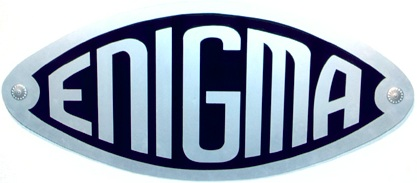
\includegraphics[width=0.38\textwidth]{pictures/enigmalogo}
  \end{center}
%\caption{A gull}
\vspace{-0pt}
\end{wrapfigure}
Die Enigma ist eine Rotor-Schlüsselmaschine, die das deutsche Militär während des Zweiten Weltkriegs zur Verschlüsselung des Nachrichtenverkehrs verwendete. Das griechische Wort $\ga\gi\gn\gi\gg\gm\ga$ bedeutet \glqq Rätsel\grqq. Obwohl die Verschlüsselungsqualität der Maschine während des Krieges mehrfach weiterentwickelt wurde, konnten die Alliierten durch enormen Aufwand zur Entschlüsselung während der meisten Zeit die deutschen Funksprüche mitlesen.

\subsection{Geschichte}

Nach dem Ersten Weltkrieg suchten die deutschen Militärs nach einem Ersatz für die inzwischen veralteten, umständlichen und unsicheren manuellen Verschlüsselungsverfahren (beispielsweise ADFGX oder Codebücher), die bis dahin verwendet wurden. Hierfür kamen maschinelle Verfahren in Betracht, weil sie eine einfachere Handhabung und eine verbesserte kryptographische Sicherheit versprachen. Basierend auf zu Beginn des 20. Jahrhunderts neu aufgekommenen Techniken, wie der elektrischen Schreibmaschine und dem Fernschreiber, kamen unabhängig voneinander und nahezu zeitgleich vier Erfinder auf die Idee des Rotor-Prinzips zur Verschlüsselung von Texten. Dabei handelt es sich um den Amerikaner Edward Hugh Hebern im Jahr 1917 (Patentanmeldung 1921), den Deutschen \textsc{Arthur Scherbius} im Jahr 1918 sowie den Niederländer \textsc{Hugo Koch} und den Schweden \textsc{Arvid Gerhard Damm} im Jahr 1919, die alle ihre Ideen zu Rotor-Chiffriermaschinen zum Patent anmeldeten.

Als Erfinder der Enigma gilt der promovierte deutsche Elektroingenieur \textsc{Arthur Scherbius} (1878--1929) dessen erstes Patent hierzu vom 23. Februar 1918 stammt. Die Enigma war zunächst als ziviles Chiffriersystem konzipiert und wurde kommerziell auf Messen --- wie 1923 auf dem internationalen Postkongress des Weltpostvereins in Bern --- zum Kauf angeboten. Gegen Ende der 1920er Jahre zeigten militärische Stellen verstärkt Interesse, so dass die Maschine bald darauf vom zivilen Markt verschwand. Gerade im Aufschwung des bis dahin eher schleppend verlaufenden Vertriebs verunglückte \textsc{Scherbius} tödlich.

Die nationalsozialistische Herrschaft hatte bereits begonnen. Da im Zuge der Aufrüstung der Wehrmacht ein zuverlässiges Verschlüsselungssystem benötigt wurde, stand dem Erfolg der Enigma nun nichts mehr im Wege.
Man schätzt, dass während des Zweiten Weltkriegs mehr als $30\,000$ Maschinen produziert wurden, einige Schätzungen reichen bis $200\,000$ Stück, vermutlich liegt die tatsächliche Zahl der eingesetzten Maschinen bei etwa $100\,000$ Stück. Im Laufe der Zeit --- bis zum Kriegsende 1945 und noch darüber hinaus --- kamen viele verschiedene Modelle und Varianten der Enigma zum Einsatz. Die meistgebrauchte war die Enigma ${1}$, die ab 1930 von der Reichswehr und später von der Wehrmacht eingesetzt wurde und das während des Zweiten Weltkriegs wohl am häufigsten benutzte Verschlüsselungsverfahren verkörpert.

\subsection{Prinzip}

Die ENIGMA I inklusive Holzgehäuse wiegt rund $\unit[12]{kg}$ und die äusseren Abmessungen (Länge $\times$ Breite $\times$ Hähe) betragen etwa $\unit[340]{mm}\times\unit[280]{mm}\times\unit[150]{mm}$. Sie sieht auf den ersten Blick wie eine Schreibmaschine aus und besteht im Wesentlichen aus der Tastatur, einem Walzensatz von drei austauschbaren Walzen (Rotoren mit einem Durchmesser von etwa $\unit[100]{mm}$) und einem Lampenfeld zur Anzeige.

\begin{figure}
\begin{center}
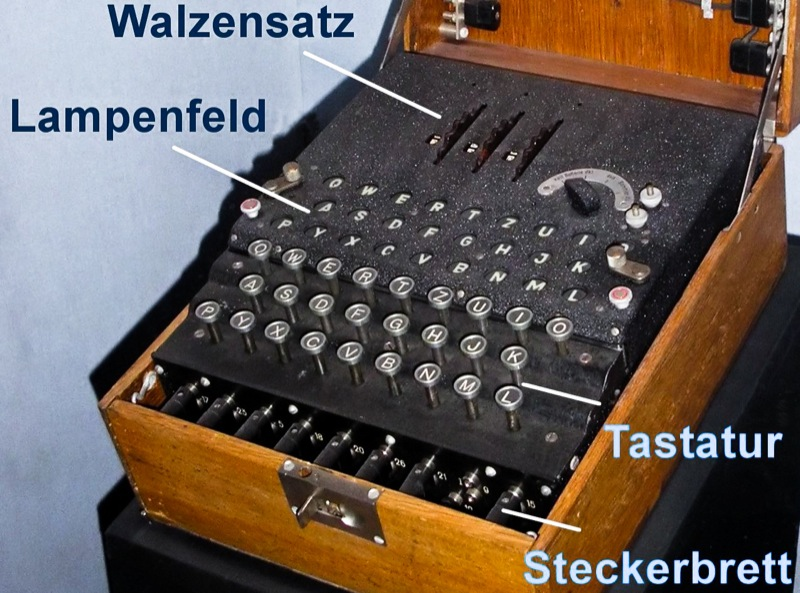
\includegraphics[width=0.5\textwidth]{pictures/enigma.jpg}
\caption{Die ENIGMA}\label{abb:enigma}
\end{center}
\end{figure}

Der Walzensatz ist das Herzstück zur Verschlüsselung. Die drei Walzen sind drehbar angeordnet und weisen auf beiden Seiten für die 26 Gro§buchstaben des lateinischen Alphabets 26 elektrische Kontakte auf, die durch 26 isolierte Drähte im Inneren der Walze paarweise und unregelmässig miteinander verbunden sind, beispielsweise (Walze III) Kontakt A mit B, B mit D, und so weiter. Drückt man eine Buchstabentaste, so flie§t elektrischer Strom von einer in der ENIGMA befindlichen 4.5-Volt-Batterie über die gedrückte Taste durch den Walzensatz und lässt eine Anzeigelampe aufleuchten. Der aufleuchtende Buchstabe entspricht der Verschlüsselung des gedrückten Buchstabens. Da sich bei jedem Tastendruck die Walzen ähnlich wie bei einem mechanischen Kilometerzähler weiterdrehen, ändert sich das geheime Schlüsselalphabet nach jedem Buchstaben.

Gibt man \texttt{otto} ein, so leuchten nacheinander beispielsweise die Lampen \texttt{PQWS} auf. Wichtig und kryptographisch stark ist, dass aufgrund der Rotation der Walzen jeder Buchstabe auf eine andere Weise verschlüsselt wird, im Beispiel das erste \texttt{o} von \texttt{otto} zu \texttt{P}, das zweite aber zu \texttt{S}. Man spricht von vielen unterschiedlichen (Geheim-) Alphabeten, die zur Verschlüsselung benutzt werden und bezeichnet dies als polyalphabetische Substitution. Würden sich die Walzen der ENIGMA nicht drehen, so bekäme man auch bei ihr nur eine einfache monoalphabetische Verschlüsselung.

\subsection{Aufbau}

In Abbildung \ref{abb:enigmaschaltung} sehen Sie den schematischen Aufbau der ENIGMA.
Rechts der drei drehbaren Walzen (5) des Walzensatzes (siehe gelb hinterlegte Zahlen in der Prinzipskizze) befindet sich die Eintrittswalze (4) (Stator), die sich nicht dreht und deren Kontakte über 26 Drähte (hier sind nur vier davon gezeichnet) mit den Buchstabentasten (2) verbunden sind. Links des Walzensatzes befindet sich die Umkehrwalze (6) (UKW), die ebenfalls feststeht.
\begin{figure}
\begin{center}
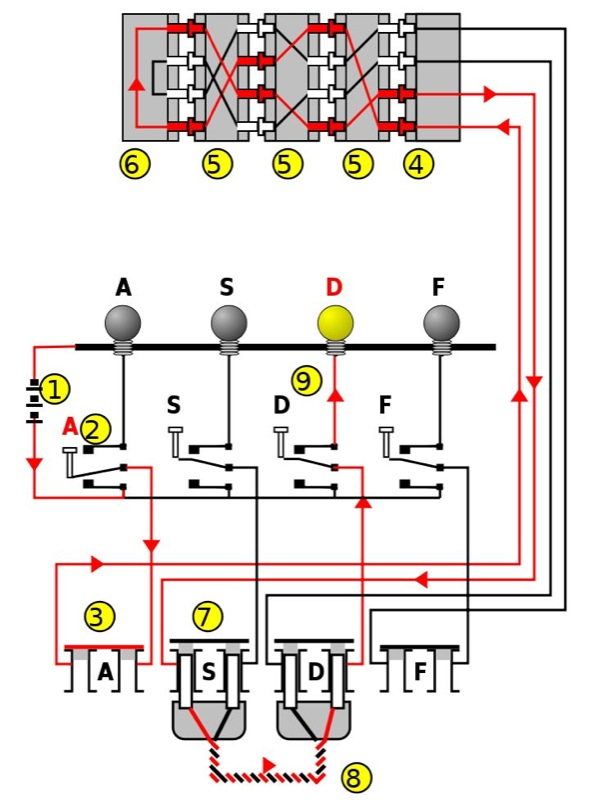
\includegraphics[width=0.35\textwidth]{pictures/enigmaschaltung.jpg}
\caption{Prinzipieller Aufbau der ENIGMA: (1) Batterie, (2) Tastatur, (3,7) Steckbrett mit (8) Stecknabel, (5) Walzensatz mit (4) Eintrittswalze und (6) Umkehrwalze sowie dem (9) Lampenfeld}\label{abb:enigmaschaltung}
\end{center}
\end{figure}
Bei ihr handelt es sich um eine Erfindung (patentiert am 21. März 1926) von \textsc{Willi Korn}, einem Mitarbeiter von \textsc{Scherbius}. Sie weist nur auf ihrer rechten Seite 26 Kontakte auf (in der Skizze sind wieder nur vier davon eingezeichnet), die paarweise miteinander verbunden sind. Die Umkehrwalze bewirkt, dass der Strom, der den Walzensatz zunächst von rechts nach links durchläuft, umgelenkt wird und ihn noch einmal durchfliesst, nun von links nach rechts. Der Strom verlässt den Walzensatz, wie er gekommen ist, wieder über die Eintrittswalze.

An der Gerätefront ist ein Steckerbrett mit doppelpoligen Steckbuchsen für jeden der 26 Buchstaben angebracht. Der Strom von der Buchstabentaste (2) wird, bevor er die Eintrittswalze (4) erreicht, über dieses Steckerbrett (3) geführt. Nach Durchlaufen des Walzensatzes fliesst er ein zweites Mal über das Steckerbrett (7,8) und bringt schlie§lich eine der 26 Buchstabenlampen (9) zum Aufleuchten.

\subsection{Schlüsselraum}

Der gesamte Schlüsselraum einer ENIGMA I mit drei aus einem Vorrat von fünf ausgewählten Walzen und einer von zwei Umkehrwalzen sowie bei Verwendung von zehn Steckern lässt sich aus dem Produkt der 120 Walzenlagen, 676 Ringstellungen, $16\,900$ Walzenstellungen und $150\,738\,274\,937\,250$ Steckermöglichkeiten berechnen. Er beträgt:
$$120\cdot676\cdot16\,900\cdot150\,738\,274\,937\,250=206\,651\,321\,783\,174\,268\,000\,000.$$
Das sind etwa $2\cdot10^{23}$ Möglichkeiten und entspricht einer Schlüssellänge von ungefähr $\unit[77]{bit}$.

Der Schlüsselraum war für diese Zeit enorm gross, ein vollständiges Durchsuchen war mit der damaligen Technologie aussichtslos. Wie wir gesehen haben, ist aber die Gr\"osse des Schlüs\-sel\-raums jedoch nur eine notwendige, aber keine hinreichende Bedingung für die Sicherheit eines kryptographischen Verfahrens. Selbst eine so simple Methode wie die einfache monoalphabetische Substitution verfügt über $26!$ mögliche Schlüssel. Das sind grob $4000\cdot10^{23}$ Schlüssel und entspricht ungefähr $\unit[88]{bit}$ und ist folglich sogar noch um etwa den Faktor $2000$ grösser als bei der ENIGMA I. Dennoch ist eine monoalphabetische Substitution leicht zu brechen.

\subsection{Entzifferung}

Die Betreiber der Schlüsselmaschine ENIGMA waren der Meinung, dass die durch sie maschinell verschlüsselten Texte (im Gegensatz zu fast allem, was bis 1918 gebräuchlich war) mit manuellen Methoden nicht zu knacken sind. Was übersehen wurde, ist, dass einer maschinellen Verschlüsselung durch maschinelle Entzifferung begegnet werden kann.

Nachdem es weder Franzosen noch Briten gelang, diese Informationen zu nutzen, und sie die ENIGMA nach wie vor als unknackbar einstuften, glückte dem 27-jährigen polnischen Mathematiker \textsc{Marian Rejewski} bei seiner Arbeit in der polnischen Dechiffrierstelle bereits im Jahre 1932 der erste Einbruch in die ENIGMA. Rejewski erriet die von den Deutschen für die militärische Variante gewählte Verdrahtungsreihenfolge. Anschliessend schaffte er es mit Hilfe seiner exzellenten Kenntnisse der Permutationstheorie, die Verdrahtung der drei Walzen (I bis III) sowie der Umkehrwalze zu erschliessen --- eine kryptoanalytische Meisterleistung, die ihn mit den Worten des amerikanischen Historikers \textsc{David Kahn}

\begin{quote}
in das Pantheon der grössten Kryptoanalytiker aller Zeiten erhebt.
\end{quote}

Die nächste Aufgabe, die gelöst werden musste, war, jeweils die richtige Walzenlage und Walzenstellung zu erschliessen. Dazu nutzte \textsc{Rejewski} zusammen mit seinen 1932 hinzugekommenen Kollegen \textsc{Jerzy R—\`{z}ycki} und \textsc{Henryk Zygalski} einen schwerwiegenden verfahrenstechnischen Fehler aus, der den Deutschen unterlief. Um eine sichere †bertragung zu gewährleisten, wurde zu dieser Zeit der Spruchschlüssel noch zweimal hintereinander gestellt und ver\-schlüs\-selt an den Anfang einer Nachricht geschrieben. Somit war der erste und vierte, der zweite und fünfte sowie der dritte und sechste Geheimtextbuchstabe jeweils demselben Klartextbuchstaben zuzuordnen. Mit Hilfe zweier speziell zu diesem Zweck gebauter Maschinen, genannt Zyklometer und Bomba, die zwei beziehungsweise sechs hintereinander geschaltete und um drei beziehungsweise eine bis fünf Drehpositionen versetzte ENIGMA-Maschinen verkörperten, konnten die polnischen Codeknacker für jede der sechs möglichen Walzenlagen feststellen, bei welchen Walzenstellungen die beobachtete Zuordnung der Buchstabenpaare möglich war und so den Suchraum gewaltig einengen. Nach Analyse mehrerer Funksprüche war der korrekte Spruchschlüssel gefunden.

Nachdem die Deutschen am 15. September 1938 ihre Verfahrenstechnik änderten und drei Monate später mit Einführung der Walzen IV und V die Anzahl der möglichen Walzenlagen von sechs auf sechzig erhöhten, konnten die Polen nicht mehr mithalten, und die ENIGMA war wieder sicher. Die nächste Hürde musste überwunden werden.

Mit diesem Anschub, konnten die britischen Kryptoanalytiker mit Ausbruch des Krieges im etwa $\unit[70]{km}$ nordwestlich von London gelegenen Bletchley Park einen erneuten Angriff auf die ENIGMA starten. Das wichtigste Hilfsmittel dabei war --- neben ihrer intellektuellen Leistungsfähigkeit und dem hohen Personaleinsatz von später zehn- bis vierzehntausend Frauen und Männern --- vor allem eine spezielle elektromechanische Maschine, genannt die Turing-Bombe, die auf der polnischen Bomba aufbaute und vom englischen Mathematiker \textsc{Alan Turing} ersonnen wurde. \textsc{Turings} Idee zur Schlüsselsuche bestand darin, durch ringförmige Verkettung von mehreren (meist zwölf) ENIGMA-Walzensätzen die Wirkung des Steckerbretts komplett abzustreifen. Dadurch gelang es ihm, die praktisch unüberschaubare Anzahl von Verschlüsselungsmöglichkeiten, auf die die deutschen Kryptographen ihre Hoffnungen setzten, drastisch zu reduzieren.

\begin{wrapfigure}{r}{0.382\textwidth}
\vspace{0pt}
\begin{center}
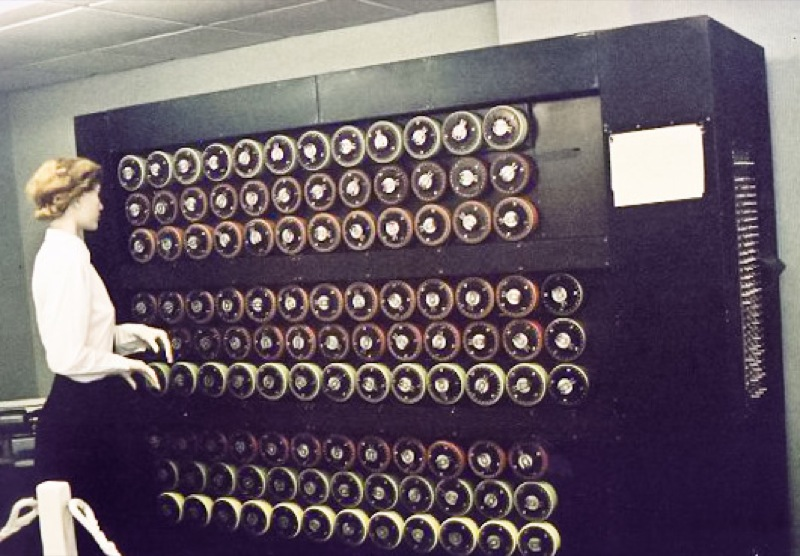
\includegraphics[width=0.38\textwidth]{pictures/turingbombe.jpg}
\caption{Die Turingbombe}
\end{center}
\vspace{0pt}
\end{wrapfigure}
Mit Hilfe der Turing-Bombe brauchte man nur noch rund sechs Stunden, um sämtliche Mög\-lich\-kei\-ten durchzutesten. Leistet man sich den Aufwand, sechzig Bomben einzusetzen, jeweils eine für jede Walzenlage, dann schrumpft die Zeit von sechs Stunden auf sechs Minuten --- eine durchaus erträgliche Zeit. Tatsächlich waren bis zum Kriegsende mehr als 210 Bomben allein in England in Betrieb.

Entscheidend wichtig für die Funktion der Bombe sind \grqq wahrscheinliche Wörter\grqq, deren Auftreten man im Text erwarten kann; fehlen diese, dann scheitert die Entzifferung.
Man profitierte von der deutschen Gründlichkeit bei der Abfassung von Routinemeldungen, wie Wetterberichte, die jeden Morgen pünktlich zur selben Zeit und vom selben Ort gesendet wurden. Aus britischer Sicht war eine täglich frisch verschlüsselte ENIGMA-Meldung, die stets mit den Worten \texttt{WETTERVORHERSAGEBEREICHSIEBEN} begann, ähnlich wertvoll wie es eine direkte öffentliche Bekanntgabe des jeweils gültigen Tagesschlüssels gewesen wäre. So wurde beispielsweise der ENIGMA-Schlüssel vom \glqq D-Day\grqq\ durch das Wort \texttt{WETTERVORHERSAGEBISKAYA}, den die britischen Kryptoanalytiker leicht erraten konnten und korrekt vermuteten, in weniger als zwei Stunden nach Mitternacht gebrochen.
Nun kamen auch die Amerikaner zu Hilfe, die ab April 1943 mehr als 120 Stück Hochgeschwindigkeitsvarianten der Turing-Bombe produzierten. Danach waren die deutschen U-Boote nie mehr sicher. Unmittelbare Folge der amerikanischen Entzifferungen war die Versenkung von neun der zwölf deutschen U-Tanker (\glqq Milchkühe\grqq) innerhalb weniger Wochen im Sommer 1943. Dies führte zu einer Schwächung aller Atlantik-U-Boote, die nun nicht mehr auf See versorgt werden konnten, sondern dazu die lange und gefährliche Heimreise durch die Biskaya zu den U-Boot-Stützpunkten an der französischen Westküste antreten mussten.

\subsection{Lernprogramm}
Das Innenleben der Enigma erleben und mehr zur Entschlüsselungstechnik kennen lernen k\"onnen bzw. sollen Sie auf MathePrisma unter
\begin{quote}
\href{http://www.matheprisma.uni-wuppertal.de/Module/Enigma/index.htm}{\texttt{MathePrisma Enigma}}
\end{quote}
Dort kann auch während des Moduls eine Java-Enigma benutzt werden.

\clearpage

\section{Data Encryption Standard}
\subsection{Binärcodes}

\begin{wrapfigure}{r}{0.3\textwidth}
\vspace{-26pt}
  \begin{center}
    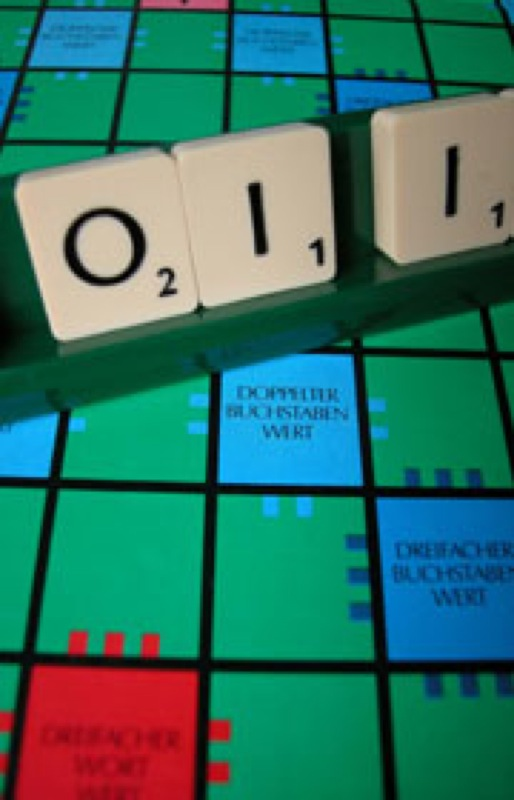
\includegraphics[width=0.2\textwidth]{pictures/scrabble}
  \end{center}
%\caption{A gull}
\vspace{-0pt}
\end{wrapfigure}
Auf einem Rechner werden alle Daten als Bit-Folgen dargestellt (binär codiert). Der Data Encryption Standard (DES) verschlüsselt solche Bit-Folgen.

Eine der gebräuchlichsten Binärcodierungen ist ASCII (American Standard Code for Information Interchange). Im ASCII wird je ein Zeichen durch ein Byte (= 8 Bits) codiert.
\begin{ueb}
Wie viele verschiedene Zeichen k\"onnen mit ASCII codiert werden?
\end{ueb}

Abbildung \ref{abb:asciibin} auf Seite \pageref{abb:asciibin} zeigt einen kleinen Auszug aus ASCII (in blau ist jeweils als Dezimalzahl angegeben, welchen Wert die Bit-Folge hat, wenn man sie als Zahl im Dualsystem interpretiert).

\begin{ueb}
Verwandle folgendes Binärwort zurück:
\begin{quote}
\texttt{01100110 01100101 01101001 01110011}\\
\texttt{01110100 01100101 01101100}
\end{quote}
\end{ueb}

\begin{figure}
\begin{center}
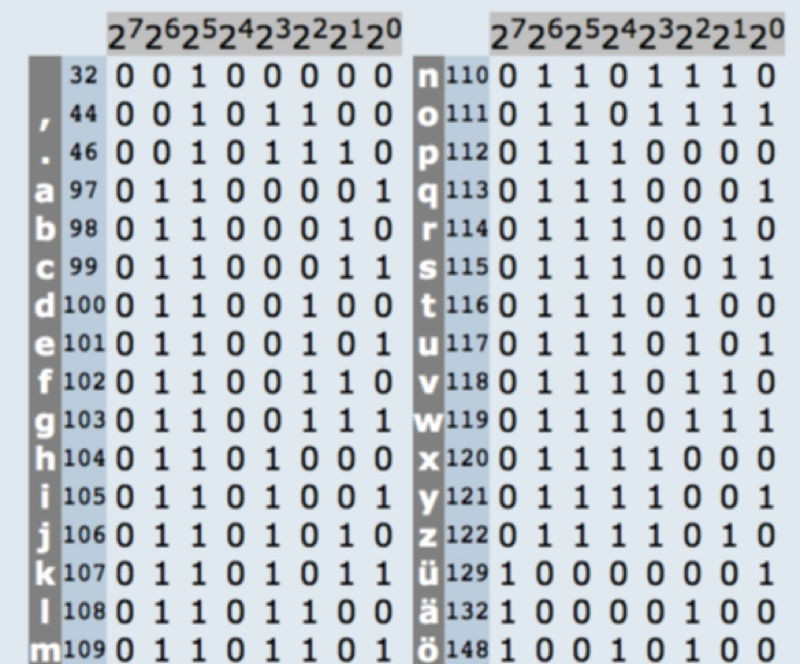
\includegraphics[width=0.5\textwidth]{pictures/ascii}
\end{center}
\caption{Auszug aus ASCII binär}\label{abb:asciibin}
\end{figure}

Der Deutsche \textsc{Horst Feistel} wurde am 30. Januar 1915 in Berlin geboren. 1934 emigrierte er nach Amerika. Wegen seiner kryptographischen Forschungen legte ihm die NSA (National Security Agency) immer wieder Steine in den Weg. Bei IBM in New York entwickelte er schliesslich in den siebziger Jahren das Prinzip der Feistel-Netzwerke, Grundlage einiger bedeutender Verschlüsselungsverfahren. 
\textsc{Feistel} starb 1990.

Zurück zu ASCII stellen wir fest, dass ein so codierter Text sich nun allerdings 8-mal so lang darstellt wie der ursprüngliche (uncodierte) Text. Man kann ihn kürzer darstellen, wenn man für je vier Bits eine Hexadezimalziffer schreibt. Denn vier Bits stellen genau die Zahlen von 0 bis 15 dar:
\begin{align*}
0000 &= 0\\
0001 &= 1\\
0010 &= 2\\
0011 &= 3\\
\dots\\
1101 &= 13\\
1110 &= 14\\
1111 &= 15
\end{align*}
Man verwendet dafür die Ziffern
$$0,1,2,3,4,5,6,7,8,9,A,B,C,D,E,F.$$
Um die unübersichtlichen Bit-Folgen eines ASCII-codierten Textes kürzer zu schreiben, stellt man jedes Byte durch zwei Hex-Ziffern dar, eine für die ersten und eine für die letzten vier Bits.
Abbildung \ref{abb:ascii} auf Seite \pageref{abb:ascii} zeigt noch einmal den Ausschnitt aus ASCII. Für die hexadezimale Schreibweise benätigt man statt 8 nur zwei Ziffern.
\begin{figure}
\begin{center}
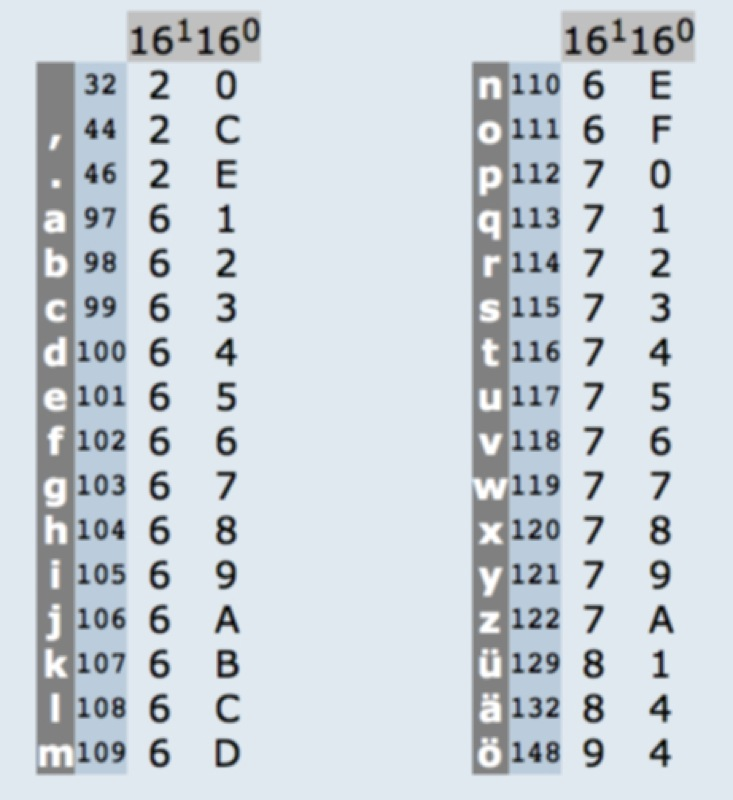
\includegraphics[width=0.5\textwidth]{pictures/asciihex}
\end{center}
\caption{Auszug aus ASCII hexadizimal}\label{abb:ascii}
\end{figure}
\begin{ueb}
Kannst du folgendes binärcodiertes, mit Hex-Ziffern dargestelltes Wort zurückwandeln? 
\begin{quote}
\texttt{6C 75 63 69 66 65 72}
\end{quote}
\end{ueb}
Lucifer ist der Name eines Ver\-schlüs\-se\-lungs\-ver\-fahrens, das \textsc{Horst Feistel} und \textsc{Don Coppersmith} 1973 im \textsc{Thomas J. Watson} Laboratory von IBM in New York entwickelten. Die NSA (National Security Agency) wurde gebeten, die Sicherheit der Lucifer-Verschlüsselung zu beurteilen. Die NSA scheint von der Sicherheit Lucifers beeindruckt gewesen zu sein: Sie bestand darauf, die Zahl der Schlüssel zu begrenzen (das Verfahren also künstlich unsicherer zu machen).
\begin{quote}
\glqq Offenbar glaubte die NSA, eine solche Obergrenze würde im zivilen Gebrauch die Sicherheit gewährleisten, weil keine nichtmilitärische Organisation einen Computer besass, der leistungsfähig genug war, um jeden möglichen Schlüssel in einem vernünftigen Zeitraum zu prüfen. Die NSA selbst jedoch, die über die besten Computer der Welt verfügt, würde gerade noch in der Lage sein, in den verschlüsselten Nachrichtenverkehr einzubrechen.\grqq

(aus: \textsc{Simon Singh}, Geheime Botschaften)
\end{quote}
Diese Version von Lucifer mit beschränkter Schlüsselzahl wurde 1976 unter dem Namen Data Encryption Standard (DES) der offizielle amerikanische Verschlüsselungsstandard.

\begin{longtable}{|c|c|c|c||c|c|c|c|}
\hline
Dez & Hex & Okt & Zeichen & Dez & Hex & Okt & Zeichen\\
\hline
0 & 0x00 & 000 & NUL & 32 & 0x20 & 040 & SP\\
1 & 0x01 & 001 & SOH & 33 & 0x21 & 041 & ! \\
2 & 0x02 & 002 & STX & 34 & 0x22 & 042 & "'\\
3 & 0x03 & 003 & ETX & 35 & 0x23 & 043 & \# \\
4 & 0x04 & 004 & EOT & 36 & 0x24 & 044 & \$ \\
5 & 0x05 & 005 & ENQ & 37 & 0x25 & 045 & \% \\
6 & 0x06 & 006 & ACK & 38 & 0x26 & 046 & \& \\
7 & 0x07 & 007 & BEL & 39 & 0x27 & 047 & ' \\
8 & 0x08 & 010 & BS & 40 & 0x28 & 050 & (  \\
9 & 0x09 & 011 & TAB & 41 & 0x29 & 051 &  ) \\
10 & 0x0A & 012 & LF & 42 & 0x2A & 052 & * \\
11 & 0x0B & 013 & VT & 43 & 0x2B & 053 & + \\
12 & 0x0C & 014 & FF & 44 & 0x2C & 054 & , \\
13 & 0x0D & 015 & CR & 45 & 0x2D & 055 & - \\
14 & 0x0E & 016 & SO & 46 & 0x2E & 056 & . \\
15 & 0x0F & 017 & SI & 47 & 0x2F & 057 & / \\
16 & 0x10 & 020 & DLE & 48 & 0x30 & 060 & 0 \\
17 & 0x11 & 021 & DC1 & 49 & 0x31 & 061 & 1 \\
18 & 0x12 & 022 & DC2 & 50 & 0x32 & 062 & 2 \\
19 & 0x13 & 023 & DC3 & 51 & 0x33 & 063 & 3 \\
\hline
\end{longtable}

\begin{longtable}{|c|c|c|c||c|c|c|c|}
\hline
Dez & Hex & Okt & Zeichen & Dez & Hex & Okt & Zeichen\\
\hline
20 & 0x14 & 024 & DC4 & 52 & 0x34 & 064 & 4 \\
21 & 0x15 & 025 & NAK & 53 & 0x35 & 065 & 5 \\
22 & 0x16 & 026 & SYN & 54 & 0x36 & 066 & 6 \\
23 & 0x17 & 027 & ETB & 55 & 0x37 & 067 & 7 \\
24 & 0x18 & 030 & CAN & 56 & 0x38 & 070 & 8 \\
25 & 0x19 & 031 & EM & 57 & 0x39 & 071 & 9 \\
26 & 0x1A & 032 & SUB & 58 & 0x3A & 072 & : \\
27 & 0x1B & 033 & ESC & 59 & 0x3B & 073 & ; \\
28 & 0x1C & 034 & FS & 60 & 0x3C & 074 & "< \\
29 & 0x1D & 035 & GS & 61 & 0x3D & 075 & =\\
30 & 0x1E & 036 & RS & 62 & 0x3E & 076 & "> \\
31 & 0x1F & 037 & US & 63 & 0x3F & 077 & ? \\
64 & 0x40 & 100 & @ & 96 & 0x60 & 140 & ` \\
65 & 0x41 & 101 & A & 97 & 0x61 & 141 & a \\
66 & 0x42 & 102 & B & 98 & 0x62 & 142 & b \\
67 & 0x43 & 103 & C & 99 & 0x63 & 143 & c \\
68 & 0x44 & 104 & D & 100 & 0x64 & 144 & d \\
69 & 0x45 & 105 & E & 101 & 0x65 & 145 & e \\
70 & 0x46 & 106 & F & 102 & 0x66 & 146 & f \\
71 & 0x47 & 107 & G & 103 & 0x67 & 147 & g \\
72 & 0x48 & 110 & H & 104 & 0x68 & 150 & h \\
73 & 0x49 & 111 & I & 105 & 0x69 & 151 & i \\
74 & 0x4A & 112 & J & 106 & 0x6A & 152 & j \\
75 & 0x4B & 113 & K & 107 & 0x6B & 153 & k \\
76 & 0x4C & 114 & L & 108 & 0x6C & 154 & l \\
77 & 0x4D & 115 & M & 109 & 0x6D & 155 & m \\
78 & 0x4E & 116 & N & 110 & 0x6E & 156 & n \\
79 & 0x4F & 117 & O & 111 & 0x6F & 157 & o \\
80 & 0x50 & 120 & P & 112 & 0x70 & 160 & p \\
81 & 0x51 & 121 & Q & 113 & 0x71 & 161 & q \\
82 & 0x52 & 122 & R & 114 & 0x72 & 162 & r \\
83 & 0x53 & 123 & S & 115 & 0x73 & 163 & s \\
84 & 0x54 & 124 & T & 116 & 0x74 & 164 & t \\
85 & 0x55 & 125 & U & 117 & 0x75 & 165 & u \\
86 & 0x56 & 126 & V & 118 & 0x76 & 166 & v \\
87 & 0x57 & 127 & W & 119 & 0x77 & 167 & w \\
88 & 0x58 & 130 & X & 120 & 0x78 & 170 & x \\
89 & 0x59 & 131 & Y & 121 & 0x79 & 171 & y \\
90 & 0x5A & 132 & Z & 122 & 0x7A & 172 & z \\
91 & 0x5B & 133 & [ & 123 & 0x7B & 173 & \{ \\
92 & 0x5C & 134 & $\backslash$ & 124 & 0x7C & 174 &$\mid$\\
93 & 0x5D & 135 & ] & 125 & 0x7D & 175 & \} \\
94 & 0x5E & 136 & \^{} & 126 & 0x7E & 176 & "~ \\
95 & 0x5F & 137 & \_ & 127 & 0x7F & 177 & DEL \\
\hline
\end{longtable}

\subsection{Erste DES Schicht}
DES ist eine Block-Chiffre. Bei einer Block-Chiffre wird zum Verschlüsseln einer Nachricht diese in mehrere Blöcke gleicher Länge aufgeteilt. Jeder Block wird nach dem gleichen Prinzip verschlüsselt.
Beim DES ist die Länge der Blöcke 64 Bits = 8 Bytes.
Für die Sicherheit einer Block-Chiffre ist eine relativ grosse Blocklänge notwendig.
Enthält der letzte Block der zu verschlüsselnden Nachricht weniger als 64 Bit, so füllt man ihn mit irgendwelchen Dummy-Bits auf.
%Wir haben z.B. vorhin den ASCII-Code für das Leerzeichen verwendet (00100000).
Beim Verschlüsseln von Bit-Folgen im DES verwendet man verschiedene Standard-Operationen, die wir jetzt behandeln. 
DES arbeitet mit Blöcken von je 64 Bits = 8 Bytes. Um den Überblick nicht zu verlieren, nehmen wir hier aber immer nur 1 Byte.

Die XOR-Operation verknüpft zwei Bits nach folgenden Regeln:
$$0 \text{XOR} 0 = 0,  0 \text{XOR} 1 = 1,  1 \text{XOR} 0 = 1,  1 \text{XOR} 1 = 0$$
oder kurz:
\begin{table}[h!]
\centering
\begin{tabular}{|c|c|c|}
\hline
\rowcolor{Gray}\spaltenheight  \text{XOR} & 0 & 1 \spaltensep \hline
\rowcolor{lightyellow}\spaltenheight0 & 0 & 1\spaltensep \hline
\rowcolor{Gray}\spaltenheight 1 & 1 & 0\spaltensep \hline
\end{tabular}
\caption{XOR}
\end{table}	
Bei zwei Bit-Folgen gleicher Länge wendet man XOR auf jede Position einzeln an. Das Ergebnis ist wieder eine Bit-Folge.
\begin{ueb}
Bestimme das Ergebnis der XOR-Operation.
$$\texttt{01000101}\oplus\texttt{00110011}$$
\end{ueb}

Eine andere wichtige Manipulation von Bit-Folgen ist, die Positionen der einzelnen Bits zu vertauschen. Man sagt: die Bit-Folge wird durch eine Permutation auf eine neue Bit-Folge abgebildet.
Eine Permutation wird einfach durch Aufzählen der neuen Positionen angegeben:
Dies ist die Permutation
$$( \;2\; 3\; 1\; 8\; 5\; 4\; 6\; 7\; )$$
\begin{bsp}
Die 8-Bit-Folge
$$1 0 0 1 1 0 1 0$$
wird abgebildet auf 
$$0 1 0 0 1 1 0 1$$
\end{bsp}

\begin{ueb}
Gib die durch $(\;4\; 5\; 2\; 3\; 1\; 6\; 8\; 7\;)$ permutierte Folge von $10010100$ an.
\end{ueb}
Das DES verwendet insgesamt drei verschiedene Permutationen, welche mit IP, PI und P bezeichnet werden. IP und PI permutieren 64-Bit-Folgen, P permutiert 32-Bit-Folgen. Ausserdem verwendet DES noch Varianten von Permutationen (E, PC1, PC2), die wir später besprechen werden.
%In Tabellenform kannst du alle Permutationen  hier nachsehen.

Wie eine Zwiebel ist der DES aus mehreren Schichten aufgebaut. Wir schauen uns die erste Schicht jetzt an (siehe Abbildung \ref{abb:feistel} auf Seite \pageref{abb:feistel}).

\begin{figure}
\begin{center}
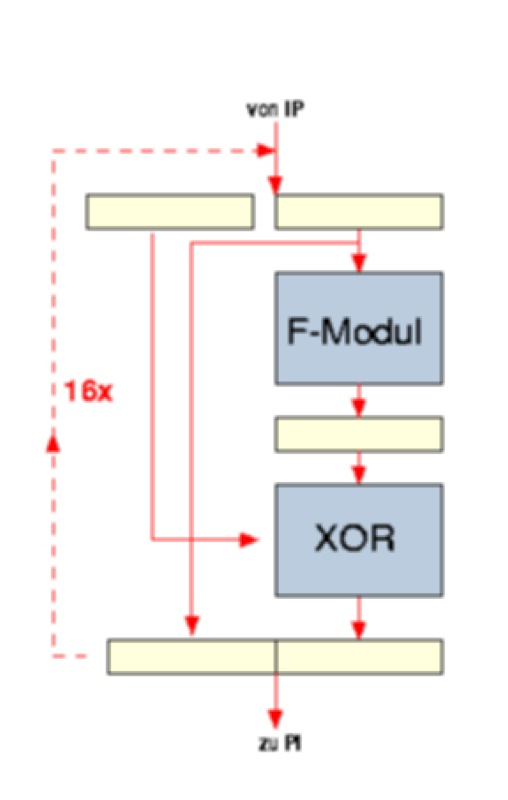
\includegraphics[width=0.35\textwidth]{pictures/zbl6}
\end{center}
\caption{Feistel-Round}\label{abb:feistel}
\end{figure}

\begin{itemize}
\item DES besteht aus einer Anfangsphase, einer mittleren Phase mit 16 Runden (Nummer 0 bis 15) und einer Endphase.
\item Die Anfangsphase besteht aus einer Permutation der gesamten Folge.
\item In den Runden werden linke und rechte Hälfte der Bit-Folge getrennt behandelt.

Jede Runde besteht aus einer Vertauschung von linker und rechter Hälfte, einer Manipulation der rechten Hälfte im F-Modul und einer XOR-Operation der manipulierten rechten mit der linken Hälfte.

Jede Runde verwendet ihren eigenen Schlüssel.
\item Die mittlere Phase wird mit einer Vertauschung von linker und rechter Hälfte abgeschlossen.
\item Die Endphase besteht aus einer abschliessenden Permutation der gesamten Folge.
\end{itemize}

Wie entschlüsselt man eine DES-verschlüsselte Nachricht? 
Das kann man herausbekommen, ohne das F-Modul näher zu kennen. 
Man muss dazu aber wissen, wie man Permutationen und XOR-Operationen rückgängig macht.

Zuerst kümmern wir uns um Permutationen. Ist b eine Bit-Folge und P eine Permutation, so bezeichnet P(b) die Bit-Folge, die aus b durch Anwendung der Permutation P entsteht.
\begin{cdef}[Inverse Permutation]{}
Die Permutation $P_2$ heisst Inverse zur Permutation $P_1$, wenn für jede Bit-Folge $b$ gilt:
$$P_2(P_1(b)) = b.$$
\end{cdef}
Wendet man also nach einer Permutation ihre Inverse an, so bleiben alle Positionen unverändert.

\begin{bsp}
Es sei
$$P_1 = ( \;2\; 3\; 1\; 8\; 5\; 4\; 6\; 7\;).$$
Dann ist
$$P_2 = ( \;3\; 1\; 2\; 6\; 5\; 7\; 8\; 4\;)$$
die Inverse von $P_1$, denn $P_2$ nach $P_1$ angewendet lässt alle Positionen unverändert.
\end{bsp}

\begin{ueb}
Gib die Inverse der Permutation
$$(\;1\;2\;6\;7\;4\;5\;8\;3\;)$$
\end{ueb}

Im DES ist die End-Permutation PI die Inverse zur Anfangspermutation IP.
%Das kannst du aus der  Tabelle ablesen. 
%Du kannst es auch im folgenden Experiment nachvollziehen, welches die mittlere Phase %der DES-Verschlüsselung einfach weglässt.

Und jetzt kümmern wir uns darum, wie man die XOR-Operation rückgängig macht.

Wie rekonstruiert man b1 aus b2 XOR b1 und b2?

\begin{ueb}
Angenommen, man kennt
$$b_2=11101001$$
und
$$b_2\oplus b_1=10111010$$
Bestimme $b_1$.
\end{ueb}

Aus der Übung sollten Sie erkennen: $b_1$ ergibt sich aus $b_2$ und $b_2\oplus b_1$ durch eine weitere XOR-Operation:
$$b_1=b_2\oplus(b_2\oplus b_1)$$

Sie haben gesehen: Zum Verschlüsseln verwendet DES insgesamt 16 Schlüssel, je einen pro Runde.

Nach dieser Vorbereitung sollte Ihnen das Entschlüsseln auch gelingen, wenn mehrere Runden durchgeführt werden. 
Eventuell hilft Ihnen auch die  formale algorithmische Beschreibung weiter.

\begin{itemize}
\item $r(b)$ bezeichnet die rechte Hälfte einer 64-Bit-Folge $b$,
\item $l(b)$ bezeichnet die linke Hälfte,
\item $b_1b_2$ bezeichnet das Aneinanderhängen zweier Bit-Folgen $b_1$ und $b_2$.

Die Zuordnung
$$b := r(b)l(b)$$
beschreibt also das Vertauschen von linker und rechter Hälfte. 
\item Mit $F(b,i)$ bezeichnen wir das Ergebnis des F-Moduls bei Anwendung auf die 32-Bit-Folge $b$ in Runde $i$.
\end{itemize}

Algorithmus:
{
\lstset{language=Java}
\begin{lstlisting}
input: 64-Bit-Folge b 
output: DES-Verschluesselung

c := IP(b)   {Anfangspermutation}
fuer i = 0,1,...,15    {Runden}
    c1 := r(c)
    c2 := l(c) XOR F(c1,i)
    c := c1c2
c := r(c)l(c)   {abschliessende Vertauschung}
c := PI(c)  {Endpermutation}
\end{lstlisting}
}

\subsection{F-Modul und S-Module}
Eine Verschlüsselung ist dann besonders gut, wenn jedes Bit des Schlüssels und jedes Bit des Originaltextes \glqq gleich starken\grqq\ Einfluss auf jedes Bit des Ergebnisses haben. 
Dafür sorgt im DES der 16-fache Einsatz des F-Moduls, die zweite Schicht der DES-Zwiebel.

Wir untersuchen jetzt die Funktionsweise des F-Moduls (siehe Abbildung \ref{abb:fmodul} auf Seite \pageref{abb:fmodul}. Das F-Modul führt folgende Operationen aus:
\begin{itemize}
\item Erweiternde Permutation der 32-Bit-Folge auf eine 48-Bit-Folge.
\item XOR-Operation mit einem 48-Bit-Schlüssel
\item Reduktion von je 6 Bit auf 4 Bit mit Hilfe der S-Module S1 bis S8.
\item Abschliessende Permutation.
\end{itemize}

\begin{figure}
\begin{center}
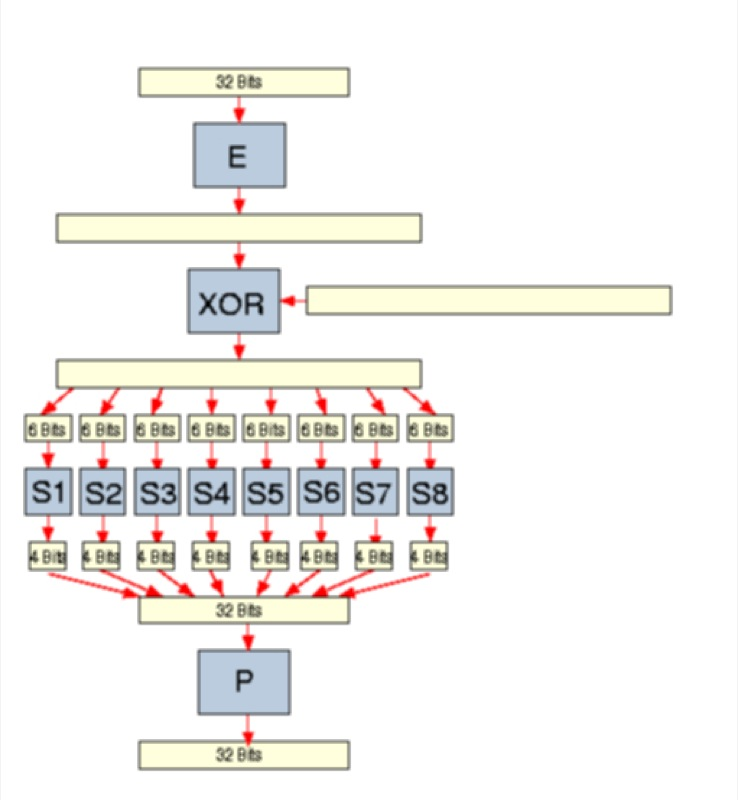
\includegraphics[width=0.55\textwidth]{pictures/fmodul5}
\end{center}
\caption{F-Modul}\label{abb:fmodul}
\end{figure}

Eine erweiternde Permutation bildet Bit-Folgen $b_1$ auf Bit-Folgen $b_2$ grösserer Länge ab. Im Gegensatz zu gewöhnlichen Permutationen werden nun einige Positionen in $b_1$ auf mehrere Positionen in $b_2$ abgebildet. Notation:
\begin{bsp}
Dies ist die erweiternde Permutation 
$$(\; 1,3\; 2\; 4,6\; 5\; ).$$
Die 4-Bit-Folge
$$1001$$
wird damit abgebildet auf
$$101010.$$
\end{bsp}

Die im F-Modul verwendete erweiternde Permutation E ist in der   Tabelle ebenso angegeben wie die abschliessende Permutation P.
Die S-Module bilden die dritte Schicht im DES. Sie verarbeiten 6-Bit-Folgen unter Verwendung von Substitutionen.

\begin{cdef}[Substitution]{}
Eine Substitution bildet jede Bit-Folge einer bestimmten Länge wieder auf eine Bit-Folge derselben Länge ab.
\end{cdef}

Substitutionen gibt man am Besten in Form einer Tabelle an, wie zum Beispiel in Abbildung \ref{abb:subst} auf Seite \pageref{abb:subst} gezeigt.
\begin{figure}
\begin{center}
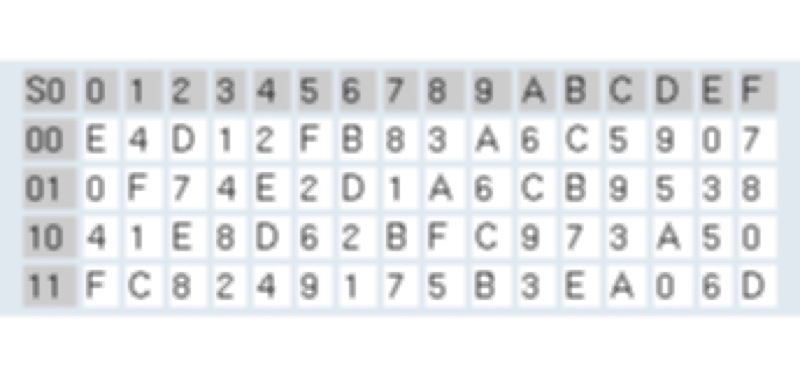
\includegraphics[width=0.5\textwidth]{pictures/subst}
\end{center}
\caption{S-Box}\label{abb:subst}
\end{figure}
Die Substitution ist fundamental verschieden von einer Permutation. Sie beruht nämlich nicht darauf, die Bits innerhalb der Bit-Folgen zu vertauschen.
Und so arbeiten die S-Module im DES:
\begin{itemize}
\item Jedes S-Modul verwendet 4 verschiedene Substitutionen auf Bit-Folgen der Länge 4. Jede Zeile der Tabelle repräsentiert eine solche Substitution.
\item Verarbeitet werden 6-Bit-Folgen
\item Anfangs- und Endbit der 6-Bit-Folge bestimmen, welche Substitution angewendet wird.
\item Die mittleren 4 Bit werden mittels dieser Substitution auf eine 4-Bit-Folge abgebildet.
\end{itemize}

\subsection{DES Schlüssel}
DES lässt nur Schlüssel mit bestimmter Parität zu.
\begin{cdef}[Parität]{}
Ist die Zahl der Einsen in einer Bit-Folge ungerade, so ist die Parität der Bit-Folge 1, andernfalls ist die Parität 0.
\end{cdef}

\begin{ueb}
Gib die Parität der Bit-Folge $0010011$ an.
\end{ueb}

Im DES verwendet der Benutzer eine von ihm gewählte (geheime) 64-Bit-Folge als Schlüssel. Diese muss er dem Empfänger, der ja entschlüsseln soll, auch mitteilen. Aus Sicherheitsgründen sollte der Schlüssel selbst wieder verschlüsselt weitergegeben werden. Eine fehlerbehaftete Übertragung des Schlüssels sollte vom Empfänger erkannt werden k\"onnen. Deshalb gibt es im DES die folgende Konvention:
\begin{quote}
Es sind nur Schlüssel zugelassen, bei welchen jedes Byte Parität 1 hat.
\end{quote}

\begin{ueb}
Was erreicht man damit?
\begin{enumeratea}
\item Fehler von einem Bit pro Byte werden immer erkannt.
\item Fehler von einem Bit pro Byte werden nur manchmal erkannt.
\item Fehler von mehreren Bit pro Byte werden immer erkannt.
\item Fehler von mehreren Bit pro Byte werden nur manchmal erkannt.
\item Fehler von einem Bit pro Byte k\"onnen korrigiert werden.
\end{enumeratea}
\end{ueb}

DES erzeugt aus dem 64-Bit-Schlüssel sechzehn 48-Bit-Schlüssel unter Verwendung von Linksverschiebungen und verringernden Permutationen.
\begin{cdef}[Linksverschiebung]{}
Die Permutation $(\;n\; 1\; 2\; \dots \;n-1\;)$ heisst Linksverschiebung um 1.
Die Permutation $(\; n-1\; n\; 1\; 2\; \dots \;n-2\;)$ heisst Linksverschiebung um 2.
\end{cdef}

\begin{cdef}[Verminderte Permutation]{}
Eine vermindernde Permutation bildet Bit-Folgen $b_1$ auf Bit-Folgen $b_2$ kleinerer Länge ab. Im Gegensatz zu gew\"ohnlichen Permutationen werden nun einige Positionen in $b_1$ ignoriert.
\end{cdef}

\begin{bsp}
Eine vermindernde Permutation von 6 Bit auf 4 Bit ist
$$(\;-\;2\;1\;-\;4\;3\;)$$
Dadurch wird $101001$ auf $1010$ abgebildet.
\end{bsp}

Die im DES zur Schlüsselgenerierung verwendeten vermindernden Permutationen PC1 und PC2 sind in der  Tabelle angegeben.
PC1 bildet 64-Bit-Folgen auf 56-Bit-Folgen ab, 
PC2 bildet 56-Bit-Folgen auf 48-Bit-Folgen ab.

\subsection{Sicherheit}
Welche Bausteine des DES tragen wie zu dessen Sicherheit bei?
Diese Frage wollen wir hier in ganz groben Zügen beantworten.

Bei einem statistischen Angriff versucht man, aus der Häufigkeit von Mustern in der verschlüsselten Nachricht auf den entschlüsselten Text zu schliessen. 
DES macht solche Angriffe aufgrund der grossen Blockgrösse von 64 Bit praktisch unmöglich.

\subsubsection{Bedeutung der Blocklänge}

Stelle dir vor, eine Nachricht wird in ASCII codiert. Auf die resultierende Bit-Folge wird eine Block-Chiffre mit nur der Länge 8 angewendet. 
Diese Nachricht kannst du dann so knacken:
\begin{enumerate}
\item Du teilst die verschlüsselte Nachricht in Blöcke zu je 8 Bit ein.
\item Du erstellst eine Tabelle, in welcher gezählt wird, wie häufig jede der 256 möglichen 8-Bit-Folgen vorkommt.
\item Die Tabelle vergleichst Du mit den durchschnittlichen Häufigkeiten der Buchstaben und Zeichen in deutschen Texten.
\item Die häufigste 8-Bit-Folge entspricht dann wohl dem 'e', die zweithäufigste dem 'n' usw.
\item Nach etwas Ausprobieren bist du am Ziel.
\end{enumerate}

\begin{ueb}
Warum kann eine Blocklänge von 64 als sicher gegen statistische Angriffe angesehen werden? Welche Aussagen sind richtig?
\begin{enumeratea}
\item 64 Bit entsprechen 8 ASCII-codierten Zeichen
\item Es gibt $256^8$ ($\approx 2 \cdot 10^{19}$) verschiedene Bit-Folgen der Länge 64.
\item Kommt im unverschlüsselten Text ein Wort aus 8 Buchstaben 
    (oder mehr) öfter vor, so wiederholt sich im 
    verschlüsselten Text eine 64-Bit-Folge genauso oft.
\item Kommt im unverschlüsselten Text ein Wort aus 8 Buchstaben 
    (oder mehr) öfter vor, so wiederholt sich auch im 
    verschlüsselten Text eine 64-Bit-Folge, aber im 
    Schnitt nur rund ein Achtel so oft.
\item Selbst wenn im verschlüsselten Text eine 64-Bit-Folge 
    häufiger vorkommt, ist es sehr schwer, ihr das richtige 
    Wort aus dem unverschlüsselten Text zuzuordnen.
\item Wenn ich eine 64-Bit-Folge im verschlüsselten Text geknackt 
    habe, so kenne ich die 8 Zeichen des Wortes. Damit finde 
    ich dann alle Stellen im verschlüsselten Text, die diesen 
    8 Zeichen entsprechen.
\end{enumeratea}
\end{ueb}

Manche Chiffren sind leicht zu knacken, wenn man die Verschlüsselungen einiger weniger Blöcke kennt ('lineare' Chiffren). 
Dass dies im DES nicht möglich ist, wird durch die S-Module und die 16 Runden erreicht. Sie machen DES zu einer hochgradig nichtlinearen Chiffre.

Um das Konzept der linearen Chiffren zu verstehen, braucht man etwas mathematische Vorbildung.

Eine Chiffre für Bit-Folgen der Länge n heisst linear (eigentlich besser: affin), falls sich die verschlüsselte Bit-Folge $b_2$ aus $b_1$ ergibt über eine Vorschrift
$$b_2 = \B{A} \cdot b_1 + \vec{c}$$
mit einer festen Matrix $\B{A}$ und einem festen Vektor $\vec{c}$. Die arithmetischen Operationen sind dabei modulo 2 zu verstehen.

Bei einer linearen Chiffre reicht es, wenn man für einen Satz von $n+1$ Bit-Folgen, welche eine Basis enthalten, die jeweiligen verschlüsselten Folgen kennt. Daraus kann man nämlich $\B{A}$ vollständig rekonstruieren.

Zum Abschluss besprechen wir noch den wohl naheliegendsten Angriff.

Man spricht von einem Brute-Force-Angriff auf eine Chiffre, wenn man einfach versucht, alle möglichen Schlüssel durchzuprobieren. 
Brute Force ist bis jetzt die erfolgreichste Angriffstaktik gegen DES.

\begin{ueb}
Wie viele verschiedene Schlüssel gibt es im DES?
\end{ueb}

Nachdem schon PCs heutzutage um die $10^{10}$ Rechenoperationen in der Sekunde leisten k\"onnen, ist es möglich, mit vielen PCs (und einige Tagen Rechenzeit) einen erfolgreichen Brute-Force-Angriff auf den DES zu fahren.

Man behilft sich deshalb mit dem Triple DES.

Beim Triple DES wird zur Verschlüsselung der DES 3-fach hintereinander angewendet, und zwar zuerst mit einem ersten Schlüssel, dann mit einem zweiten und schliesslich nochmals mit dem ersten.

\begin{ueb}
Wieviele Möglichkeiten muss man bei einem Brute-Force-Angriff jetzt in Betracht ziehen? 
Gib die richtige Gr\"ossenordnung an! (Exponent $e$ in $10^e$ )
\end{ueb}

\begin{ueb}
Wieso nicht Double-DES?
\end{ueb}

Tatsächlich ist Triple DES eine heute häufig verwendete Chiffre.

\begin{ueb}
Betrachtet wird die Bit-Folge

$$0101\q 1010\q 0110\q 0001\q 0110\q 0011\q 0110\q 1001$$

\begin{enumeratea}
\item Stelle diese Bit-Folge hexadezimal dar. 
\item Welchem Wort entspricht die Bit-Folge, wenn man je 1 Byte als ASCII-Code auffasst? 
\item Wende auf die Bit-Folge die  Permutation P des DES an.
\end{enumeratea}
\end{ueb}

\begin{ueb}
Das DES besitzt vier sog. \glqq schwache Schlüssel\grqq. Dies sind 64-Bit-Schlüssel, aus denen DES bei der Erzeugung der sechzehn 48-Bit-Schlüssel sechzehn Mal denselben Schlüssel generiert. 
Finde die vier schwachen Schlüssel. 
Hinweis: Alle Bytes der schwachen Schlüssel haben Parität 0. Es sind also eigentlich gar keine zugelassenen Schlüssel.
\end{ueb}

\begin{ueb}
Bei Triple DES werden der erste und der dritte Schlüssel identisch gewählt.
\begin{enumeratea} 
\item Welchen Grund mag diese Einschränkung haben? 
\item In nicht zu ferner Zukunft schafft man es vielleicht, das für einen Brute-Force Angriff auf das gewöhnliche DES notwendige Ausprobieren aller  Schlüssel in einer Stunde durchzuführen. 
Wie lange braucht man dann (in Jahren) für einen Brute-Force-Angriff auf Triple DES?
\end{enumeratea}
\end{ueb}

\begin{ueb}
Eine vermindernde Permutation führt zu einem Informationsverlust, da zwei unterschiedliche Bit-Folgen auf das selbe Ergebnis abgebildet werden k\"onnen.
\begin{enumeratea}
\item Gib für die vermindernde Permutation $(\;-\; 2\; 4\; 1\; 3\; -\;)$ zwei 6-Bit-Folgen an, die auf dasselbe Ergebnis abgebildet werden. 
\item Ergibt sich diese Problematik auch bei erweiternden Permutationen? 
\item Das DES ist nur sinnvoll, wenn verschiedene Bit-Folgen auch verschieden verschlüsselt werden (warum eigentlich?). 
Erläutere, warum dies tatsächlich so ist, obwohl im DES vermindernde Permutationen eingesetzt werden.
\end{enumeratea}
\end{ueb}

Die obigen Übungen stammen von der Site
\begin{quote}
    \href{http://www.matheprisma.uni-wuppertal.de/Module/DES/index.htm}{\texttt{MathePrisma DES}}
\end{quote}
Diese führt auch durch ein schönes Lernmodul.

\begin{figure}
\begin{center}
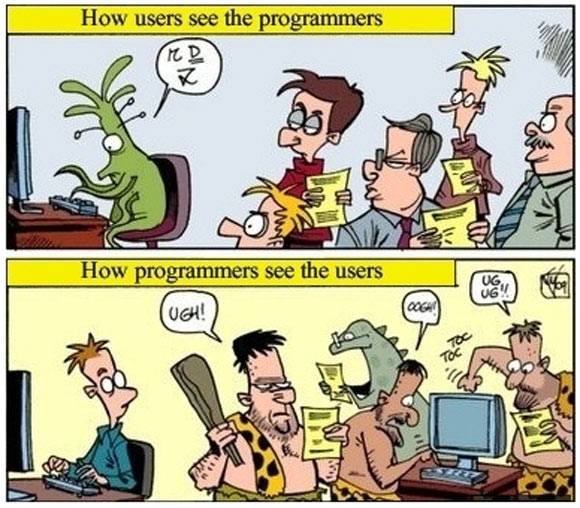
\includegraphics[width=0.382\textwidth]{pictures/users}
\end{center}
\caption{Programmers \& Users}
\end{figure}

\clearpage

\section{RSA}
\subsection{Asymmetrie}

\begin{wrapfigure}{r}{0.32\textwidth}
\vspace{-22pt}
  \begin{center}
    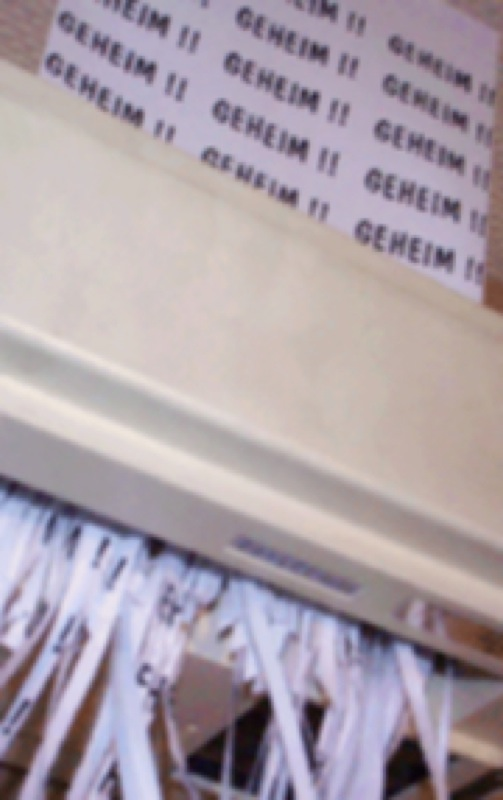
\includegraphics[width=0.26\textwidth]{pictures/rsa}
  \end{center}
%\caption{A gull}
\vspace{-22pt}
\end{wrapfigure}
Wird der Schlüssel beim Austausch abgefangen, so ist die gesamte Verschlüsselung wertlos. Lange Zeit galt diese Sicherheitslücke als unvermeidbar. Es gibt aber auch Verschlüsselungen, die ganz ohne Schlüsselaustausch auskommen. Wie geht das?

Wir denken uns für eine erste Idee, dass eine Kiste geschickt wird, die man mit einem Vorhängeschloss verschliessen kann. Dabei wird zwar die Nachricht mehrfach hin und her geschickt, es wird aber kein Schlüssel ausgetauscht; das geht so:
\begin{enumerate}
\item Alice verschliesst die Kiste mit ihrem Schloss und schickt sie an Bob.
\item Bob verschliesst die Kiste ein zweites mal mit seinem Schloss und schickt sie Alice zurück.
\item Alice entfernt ihr Schloss mit ihrem Schlüssel und schickt die Kiste wieder an Bob.
\item Bob kann die Kiste mit seinem Schlüssel öffnen.
\end{enumerate}
\begin{ueb}
Das Verfahren geht natürlich einfacher, ohne die Kiste hin und her schicken zu müssen. Nämlich \dots
\end{ueb}
Bob muss also nur dafür sorgen, dass Alice ein Schloss von ihm hat. Das ist kein Problem, denn verschliessen kann man ja ohne Schlüssel. Aber nur Bob kann mit dem Schlüssel die Kiste wieder öffnen.

\subsection{Einwegfunktionen}
Eine Einwegfunktion ist eine Funktion, die einfach zu berechnen aber sehr schwer umkehrbar ist. Im täglichen Leben findet man viele \glqq Einwegfunktionen\grqq:
\begin{itemize}
\item sich ein Bein brechen
\item Zahnpasta aus der Tube drücken
\end{itemize}

\begin{cdef}[one-way function]{}
Eine one-way-function ist eine injektive Funktion
$$f:X\to Y$$
so dass gilt:
\begin{itemize}
\item Es gibt ein effizientes Verfahren zur Bestimmung von $y=f(x)\q\forall x\in X$.
\item Die Umkehrung ist praktisch unmöglich, d.h. es gibt kein effizientes Verfahren zur Bestimmung von $x=f^{-1}(y)\q\forall y\in f(X)$.
\end{itemize}
\end{cdef}

\begin{bem}
Das heisst nicht, dass eine Einwegfunktion nicht umkehrbar ist, die Umkehrung ist nur so schwierig, dass sie praktisch nicht umzusetzen ist.
Das bedeutet dann aber, dass eine Verschlüsselung durch eine Einwegfunktion weder von Unbefugten geknackt, noch vom rechtmässigen Empfänger der Nachricht entschlüsselt werden kann.
Man braucht also etwas anderes: Einwegfunktionen mit Falltür.
\end{bem}

\begin{cdef}[one-way-trap-door function]{}
Eine trap-door one-way-function ist eine injektive Funktion $f:X\to Y$ für die gilt:
\begin{itemize}
\item Es gibt effiziente Verfahren zur Berechnung von $y=f(x)\q\forall x\in X$ und $x=f^{-1}(y)\q\forall y\in f(X)$.
\item Das Verfahren zur Berechnung von $f^{-1}$ kann nicht aus dem Verfahren zur Berechnung von $f$ hergeleitet werden. Man benötigt eine (geheime) Zusatzinformation.
\end{itemize}
\end{cdef}

\begin{bsps}
Einwegfunktionen mit Falltür aus dem Leben gegriffen:
\begin{itemize}
\item Vorhängeschloss zuschnappen lassen
\item Brief in einen Briefkasten werfen.
\end{itemize}
\end{bsps}

Die entscheidende Frage für uns ist also, wie man nun eine konkrete Einwegfunktion mit Falltür findet oder erfindet, um eine Nachricht zu verschlüsseln.

\subsection{Idee von RSA}
Wir wissen, dass das Produkt zweier Primzahlen einfach zu berechnen ist. Wie sieht es mit der Umkehrung aus?
\begin{ueb}
Bestimme die Primfaktorzerlegung von

\begin{minipage}{0.2\textwidth}
\begin{enumeratea}
\item 21
\item 65
\end{enumeratea}
\end{minipage}
\begin{minipage}{0.4\textwidth}
\begin{enumeratea}
\setcounter{enumi}{2}
\item 14803
\item 12863273
\end{enumeratea}
\end{minipage}
\end{ueb}

Je grösser die Zahl, desto aufwändiger kann es werden, ihre Primfaktorzerlegung zu bestimmen. Kann es werden, denn dies muss nicht uneingeschränkt sein.
\begin{ueb}\label{primeasy}
Bestimme die Primfaktorzerlegung von $2\,469\,135\,782$.
\end{ueb}
†bung \ref{primeasy} ist einfach, weil einer der beiden Primfaktoren sehr klein ist. Im Allgemeinen gilt aber, dass das Multiplizieren zweier grossen Primzahlen eine Einwegfunktion mit Falltür ist.
Darauf beruht das bekannteste asymmetrische Verschlüsselungsverfahren RSA. Wählt nämlich Bob zwei grosse Primzahlen $p$ und $q$ und hält diese geheim, so kann er das Produkt $N=p\cdot q$ veröffentlichen ohne in Gefahr zu laufen, dass jemand die Primfaktoren $p$ und $q$ bestimmen kann.
Den Namen hat das Verfahren von Ronald Rivest, Adi Shamir und Leonard Adleman, den drei Männern, die es 1977 erfunden haben.
\begin{figure}
\begin{center}
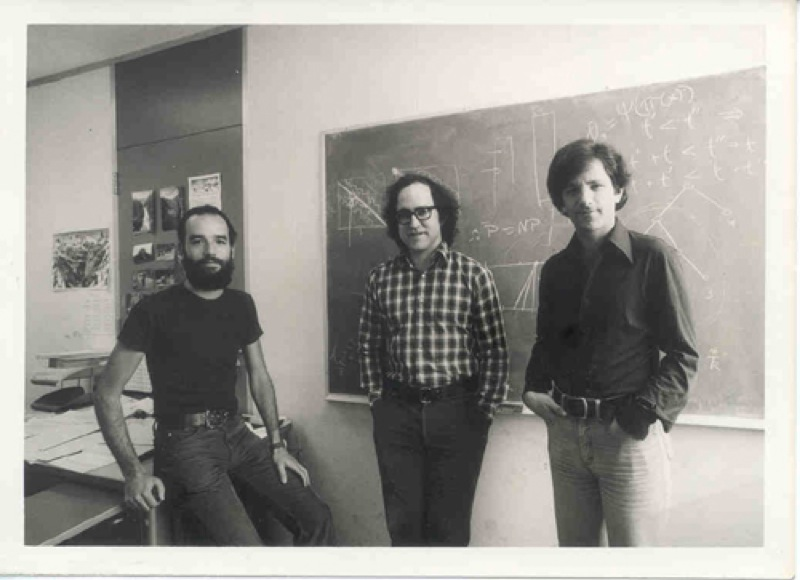
\includegraphics[width=0.618\textwidth]{pictures/rsaleute}
\end{center}
\caption{Shamir, Rivest und Adleman}
\end{figure}
RSA ist ein asymmetrisches Verfahren, es gibt also einen public key und einen private key. Beide werden über Primzahlen gebildet. Ausserdem geht in das Verfahren die Modulo-Rechnung ein.

Für die Erzeugung der beiden Schlüssel wählt man zunächst zwei grosse Primzahlen $p$ und $q$. Diese werden multipliziert und man erhält $N=p\cdot q$. Diese Zahl  $N$ sowie eine weitere (fast) beliebig wählbare Zahl  $e$ (encipher = verschlüsseln) bilden den public key. Eine dritte Zahl $d$ (decipher = entschlüsseln), zu deren Berechnung wir später kommen, ist der private key.
Verschlüsselt wird durch
$$C\equiv M^e\mod N.$$
Die Zahlen $N$ und $e$ sind der public key. $M$ ist der Klartext (Message), $C$ der verschlüsselte Text (Cipher).
\begin{ueb}
Nehmen wir an, du willst an Alice die Nachricht $L$ schicken. Alices public key sei $(187, 7)$, also $N=187$ und $e=7$.
Das $L$ lautet in ASCII $01001100$, das entspricht der Dezimalzahl $76$. Die Nachricht lautet also \dots.
\end{ueb}
\noindent Zum Entschlüsseln benötigt man den geheimen Schlüssel $d$. Entschlüsselt wird damit durch $$M\equiv C^d\mod N$$
\begin{ueb}
Und umgekehrt? Angenommen, dein \"offentlicher Schlüssel ist $(187, 7)$. Du erhältst die damit verschlüsselte Nachricht $C=142$. Um diese zu entschlüsseln, ben\"otigst du deinen private key. Der ist in diesem Fall $d=23$. Wie $d$ berechnet wird, kommt später.
\end{ueb}

\begin{ueb}
Probier es mit dem Taschenrechner aus obiger Aufgabe aus. Verschlüssele verschiedene Zahlen und entschlüssele sie direkt wieder. Versuche Zahlen, die kleiner sind als $N=187$ und Zahlen, die gr\"osser sind!
\end{ueb}

\begin{bem}
Das funktioniert allerdings nur, wenn die Nachricht  $M$ (als Zahl) kleiner ist als $N$. Das ist allerdings keine Einschränkung. Will man eine Nachricht verschlüsseln, deren Zahlenwert zu gross ist, so teilt man sie in kleinere Blöcke und verschlüsselt jeden Block einzeln.
\end{bem}

\begin{bsp}
Um es einfach zu halten, codieren wir: Leerzeichen = 00, A = 01, B = 02, \dots, Z = 26.
Mit dem Schlüssel (N, e) = (2773, 17) wird die Nachricht:
$$05\q 18\q 18\q 01\q 18\q 05\q 00\q 08\q 21\q 13\q 01\q 14\q 21\q 13\q 00\q 05\q 19\q 20$$
in 3er-Blöcke geteilt (die sind sicher kleiner als $N$):
$$051\q 818\q 011\q 805\q 000\q 821\q 130\q 114\q 211\q 300\q 051\q 920$$	
und verschlüsselt zu (mit führenden Nullen auf vier Stellen aufgefüllt):
$$2236\q 2000\q 1725\q 0542\q 0000\q 0436\q 1988\q 1684\q 1064\q 0567\q 2236\q 0948$$
\end{bsp}
Nun zur Frage, wie man den private key $d$ berechnet.
\begin{bem}
Der private key $d$ errechnet sich aus der Gleichung
$$e\cdot d\mod(p-1)(q-1)=1$$
\end{bem}
\noindent Grundlage zur Berechnung von $d$ ist folgender Satz, der garantiert, dass es eine solche Zahl überhaupt gibt --- vorausgesetzt die Zahl $e$ hat eine bestimmte Eigenschaft\dots

\begin{csatz}[Existenz eines modular Inversen]{}
Sind $a,b\in\mZ$ teilerfremd, so gibt es eine ganze Zahl $c$, so dass
$$b\cdot c\mod a\equiv1$$
\end{csatz}

\begin{cdef}[Modular Inverses]{}
Mit den Bezeichnungen aus obigem Satz sagt man, $b$ ist modulo $a$ invertierbar und nennt $c$ die modular Inverse von $b$.
\end{cdef}

\begin{ueb}
Finde das modular Inverse Element $c$ zu $3$ modulo $5$.
\end{ueb}
\noindent In unserem Fall sind wir gerade daran interessiert $e$ modulo $(p-1)(q-1)$ zu invertieren. Das heisst insbesondere, dass $e$ und $(p-1)(q-1)$ teilerfremd sein müssen.

Und wie berechnet man die modulare Inverse nun? Ein Verfahren für diese Berechnung ist in dem Beweis zu obigem Satz versteckt. Deswegen folgt er hier ausführlich. Er erfolgt in drei Schritten:
\begin{enumerate}
\item Mit dem euklidschen Algorithmus zur Bestimmung des ggT
\item Summendarstellung des ggT von von entsprechenden Vielfachen der beiden Zahlen (erweiterter Euklidscher Algorithmus)
\item Betrachtung des Falls, dass $a$ und $b$ teilerfremd sind, d.h. dass ihr ggT $1$ ist.
\end{enumerate}
Wir wissen bereits, wie man den ggT von zwei Zahlen mit dem Euklidschen Algorithmus bestimmt. Der ggT ist der letzte, nichttriviale Rest.
\begin{ueb}
Schreibe allgemein das Verfahren des Euklidschen Algorithmus für zwei Zahlen $a$ und $b$, sagen wir bis zu Schritt fünf, auf.
\end{ueb}
\noindent Rechnet man nun rückwärts und ersetzt die Reste durch entsprechende Ausdrücke, so erhält man eine Vielfachendarstellung von $a$ und $b$ für ihren ggT.

\begin{ueb}
Zeige dies.
\end{ueb}

\begin{csatz}[Satz von Bézout]{}
Zu zwei Zahlen $a,b\in\mZ$ gibt es immer Zahlen $x,y\in\mZ$, so dass
$$\ggT(a,b)=x\cdot a+y\cdot b.$$
\end{csatz}

\begin{proof}
Damit ist Schritt drei nur noch Formsache. Für teilerfremde $a,b$ gilt jetzt
$$1=x\cdot a+ y\cdot b$$
Dies gilt natürlich auch noch modulo $a$ bzw. $b$, da $x\cdot a\mod a=0$ ist.
$$x\cdot a+y\cdot b\mod a=y\cdot b\mod a=1.$$
Also ist $c=y$ modulo $a$ invers zu $b$.
\end{proof}

\begin{bem}
Dieses
\marginnote{
\qrcode{
https://www.youtube.com/watch?v=9Nl6KP7pSv4}
}
$c$ lässt sich mit dem Euklidschen Algorithmus berechnen.
\end{bem}
\noindent Hat man also die Vielfachensummendarstellung
$$1=\ggT((p-1)(q-1),e)=x\cdot(p-1)(q-1)+y\cdot e$$
bestimmt, so ist die kleinste positive Zahl der Form
$$y+k\cdot(p-1)(q-1)$$
gleich dem private key $d$.
\begin{bem}
Mit Hilfe des euklidischen Algorithmus' kann man also den private key $d$ bestimmen.
Kennt man die beiden Primzahlen $p$ und $q$, so ist es also einfach, $d$ zu berechnen und damit dann die mit $N$ und $e$ verschlüsselten Nachrichten zu entschlüsseln. Allerdings ist es nahezu unmöglich, $d$ zu berechnen, ohne $p$ und $q$ zu kennen.
\end{bem}
Aber warum funktioniert das Verfahren denn nun überhaupt? Warum kommt wirklich wieder der Klartext heraus, mit anderen Worten: warum gilt
$$C^d\mod N=M?$$
Wir erinnern uns, wie der Cipher-Text entstanden ist,
$$C^d\mod N = (M^e)^d\mod N= M^{e\cdot d}\mod N.$$
und k\"onnen daher die Frage umformulieren: gilt tatsächlich
$$M^{e\cdot d}\mod N=M?$$
Die Antwort auf diese Frage lautet natürlich ja. Für den Beweis brauchen wir den kleinen Satz von Fermat, der ein Spezialfall des Satzes von Euler ist.
Zur einfachen Formulierung des Satzes brauchen wir die sogenannte Euler'sche $\Phi$-Funktion.

\begin{cdef}[Euler'sche phi-Funktion]{}
Für eine natürliche Zahl $n$ ist $\Phi(n)$ die Anzahl der natürlichen Zahlen $\leq n$, deren gr\"osster gemeinsamer Teiler mit $n$ gleich $1$ ist. Man nennt $\Phi$ die Euler'sche $\Phi$-Funktion.
\end{cdef}

\begin{csatz}[Euler-phi einer Primzahl]{}
Ist $p$ prim, dann gilt
$$\Phi(p)=p-1.$$
\end{csatz}
\begin{proof}[Beweis]
Da $p$ teilerfremd zu $1,2,3,\dots,p-1$ ist folgt der Satz.
\end{proof}

\begin{csatz}[Satz von Euler]{}
Sind $m,n\in\mN$ teilerfremd, so gilt
$$m^{\Phi(n)}\mod n=1.$$
\end{csatz}
\noindent Ein interessanter Spezialfall, den man auch zum Beweis der Korrektheit der Entschlüsselung verwenden kann, ist
\begin{csatz}[Multiplikativität der Euler'schen phi-Funktion]
Sind $p,q$ zwei verschiedene Primzahlen, so ist
$$\Phi(p\cdot q)=(p-1)(q-1).$$
\end{csatz}
\noindent Ist $m$ teilerfremd zu $p\cdot q$, so gilt nach dem Satz von Euler
$$m^{(p-1)(q-1)}\mod pq=1.$$
\begin{csatz}[Kleiner Satz von Fermat]{}
Sei $m$ eine natürliche Zahl und teilerfremd zur Primzahl $p$. Dann gilt
$$m^{p-1}\mod p=1.$$
\end{csatz}
Der
\marginnote{
\qrcode{
https://www.youtube.com/watch?v=mLMCAe1HRSs}
}
Beweis, dass die Entschlüsselung korrekt ist, geht damit so:
Wir wissen, dass
$$e\cdot d\mod(p-1)(q-1)=1.$$
Das heisst, es gibt ein $k\in\mZ$ mit
$$e\cdot d=k\cdot(p-1)(q-1)+1.$$
Damit
\begin{align*}
M^{e\cdot d}-M\mod p&=M^{k\cdot(p-1)(q-1)+1}-M\mod p=(M^{(p-1)})^{k(q-1)}\cdot M-M\mod p=\\
&=1^{k(q-1)}\cdot M-M\mod p=0.
\end{align*}
Dies gilt insbesondere auch, wenn $p$ ein Teiler von $M$ ist, denn dann ist $M^{e\cdot d}-M\mod p$ sowieso gleich $0$. Ferner sieht man analog, dass $M^{e\cdot d}-M\mod q=0$.
Die Primzahlen $p$ und $q$ teilen also dieselbe Zahl $M^{e\cdot d}-M$, also muss auch ihr Produkt diese Zahl teilen. Somit gilt:
$$M^{ed}\mod pq=M.$$

\subsection{RSA knacken}
Zum Schluss noch ein Beispiel, wie RSA aus Sicht des Codeknackers aussieht. Um es schon mal vorwegzunehmen: es ist ein Beispiel, in dem es dem Codeknacker leicht gemacht wird. Also keine Angst, so schnell wie hier lässt sich RSA nicht knacken\dots

\begin{bsp}
Sie haben eine RSA-verschlüsselte Nachricht abgefangen. Sie lautet
\begin{quote}
10473054210223505497035330523101828168\\
2305497093070549713322042531164705144
\end{quote}
Ausserdem wissen Sie für wen die Nachricht bestimmt ist. Der \"offentliche Schlüssel des Empfängers ist
$$N=17947,\q e=21$$
Um die Nachricht zu entschlüsseln, müssen Sie herausfinden, aus welchen beiden Primzahlen $p$ und $q$ sich $N$ zusammensetzt.
Eine erste Möglichkeit, $p$ und $q$ herauszufinden ist, bei 2 anzufangen und jede Zahl zu testen, ob sie ein Teiler von $N$ ist. Dabei kann man sich die Arbeit einfacher machen, wenn man bedenkt, dass
\begin{itemize}
\item nicht $p$ und $q$ beide gr\"osser als $\sqrt{N}$ sein k\"onnen (man braucht also \glqq nur\grqq\ die Zahlen bis $\sqrt{N}$ zu testen)
\item die beiden gesuchten Teiler von $N$ Primzahlen sind (man braucht also z.B. die geraden Zahlen gar nicht testen).
\end{itemize}
Allerdings dauert diese Suche um so länger je grösser $p$ und $q$  sind. Es scheint also geschickter zu sein, die Suche bei möglichst grossen Zahlen anzufangen, d.h. bei $\sqrt{N}$.
Wenn Sie die Zahlen $p$ und $q$ herausgefunden haben, k\"onnen Sie nun ganz normal den privaten Schlüssel  bestimmen.
\end{bsp}

\subsection{übung zu RSA mit Mathematica}
Zum
\marginnote{
\qrcode{
https://www.youtube.com/watch?v=k-mlgN6BLI0}
}
Schluss noch ein etwas grösseres Beispiel. Alice wöhle als $p$ Primzahl Nummer $1000000000$ und als $q$ Primzahl Nummer $1000005000$. Der Befehl Prime[.] des Programms Mathematica liefert ihr
$$p = 22801763489,\q	q = 22801881559.$$
Daraus folgt
$$n = pq = 519923110412508599351.$$
Nun muss sie die Zahlen $c$ und $d$ so bestimmen, dass $d$ zu $c$ invers Modulo $(p-1)(q-1)$ ist. Es ist
$r = (p-1)(q-1) = 519923110366904954304$. Sie wählt
$$c = 4699873.$$
Mithilfe des Mathematica-Befehls GCD[c, r], der den gr\"ossten gemeinsamen Teiler der beiden Zahlen $c$ und $r$ bestimmt, erhält man GCD[c, r] = 1, das heisst $c$ und $r$ sind teilerfremd. Der Mathematica-Befehl PowerMod[c,-1,r] liefert für $d$
$$d = 252883827627895253473.$$
Tatsächlich ergibt die Division
$$\frac{cd - 1}{r} = k = 2285957.$$
Alice ver\"offentlicht nun in der Zeitung die beiden Zahlen
$$n = 519923110412508599351,\q	c = 4699873.$$
Ihr Freund Bob hat nur darauf gewartet und beschliesst, ihr die folgende Botschaft zu schicken
\begin{center}
\texttt{
RSA IST EIN GENIESTREICH
}
\end{center}
Diesen Text übersetzt er zuerst nach ASCII in einen Block von Zahlen. Für die Grossbuchstaben A, B, C, \dots verwendet ASCII der Reihe nach die Zahlen 65, 66, 67, \dots Ein Leerschlag erhält die Zahl 32. Das ergibt folgenden Zahlenstring
$$82 83 65 32 73 83 84 32 69 73 78 32 71 69 78 73 69 83 84 82 69 73 67 72$$
Bob bildet daraus drei Zahlen $m_1, m_2, m_3$
$$m_1 = 82836532738384326973, m_2 = 78327169787369838482, m_3 = 69736772,$$
die alle kleiner als $n$ sind. Weil
$$\text{PowerMod[$m,c,n$]} = m^c\mod n$$
gilt, kann Bob mit Mathematica leicht
$$\overline{m_1} = m_1^c\mod n = 479529267290958755149$$
berechnen, und ebenso
$$\overline{m_2} = m_2^c\mod n = 428935216287316816132,$$
$$\overline{m_3} = m_3^c\mod n = 135766055009022893446.$$
Diese drei Zahlen ver\"offentlicht er in der Zeitung, in der sie Alice alsbald entdeckt. Sie berechnet nun, ebenfalls mit dem Mathematica-Befehl PowerMod sukzessive PowerMod[$m_1,d,n$], 
PowerMod[$m_2,d,n$], PowerMod[$m_3,d,n$] und findet die drei Zahlen
$$82836532738384326973,$$
$$78327169787369838482,$$
$$69736772.$$
Indem sie den ASCII Code rückwärts übersetzt, findet sie Bobs Mitteilung
\begin{center}
\texttt{
RSA IST EIN GENIESTREICH
}
\end{center}
und ist enttäuscht: So eine Banalität hätte er nun wirklich nicht zu verschlüsseln brauchen!

\clearpage

\section{Pretty Good Privacy}

PGP
\marginnote{
\qrcode{
https://www.youtube.com/watch?v=RY6C_Vs4a0Q}
}
benutzt ein sogenanntes Public-Key-Verfahren, in dem es ein eindeutig zugeordnetes Schlüsselpaar gibt:

Genutzt wird ein öffentlicher Schlüssel, mit dem jeder Daten für den Empfänger verschlüsseln und dessen Signaturen prüfen kann, und ein privater geheimer Schlüssel, den nur der Empfänger besitzt und der normalerweise durch ein Passwort geschützt ist. Nachrichten an einen Empfänger werden mit dessen öffentlichem Schlüssel verschlüsselt und können dann ausschliesslich mittels seines privaten Schlüssels entschlüsselt werden. Diese Verfahren werden auch asymmetrische Verfahren genannt, da Sender und Empfänger zwei unterschiedliche Schlüssel verwenden.

Die erste Version wurde im Jahr 1991 geschrieben und verwendete einen RSA-Al\-go\-rith\-mus zur Verschlüsselung der Daten.

Bei PGP wird aber nicht die ganze Nachricht asymmetrisch verschlüsselt, denn dies wäre viel zu rechenintensiv und es wäre nicht praktikabel, dieselbe Nachricht an mehrere Empfänger zu schicken. Stattdessen wird die eigentliche Nachricht symmetrisch und nur der verwendete Schlüssel asymmetrisch verschlüsselt (Hybride Verschlüsselung). Dazu wird jedes Mal ein symmetrischer Schlüssel (session key) zufällig erzeugt.

Dieser symmetrische Schlüssel wird dann z.B. per RSA- oder Elgamal-Kryptosystem mit dem öffentlichen Schlüssel des Empfängers verschlüsselt und der Nachricht hinzugefügt. Dadurch ist es möglich, eine Nachricht für mehrere Empfänger gleichzeitig zu verschlüsseln.

\hfill(Quelle: Wikipedia, 2020)

Schematisch
habe ich dies so wie in Abbildung \ref{fig:pgp} auf Seite \pageref{fig:pgp} illustriert.
\begin{figure}
    \centering
    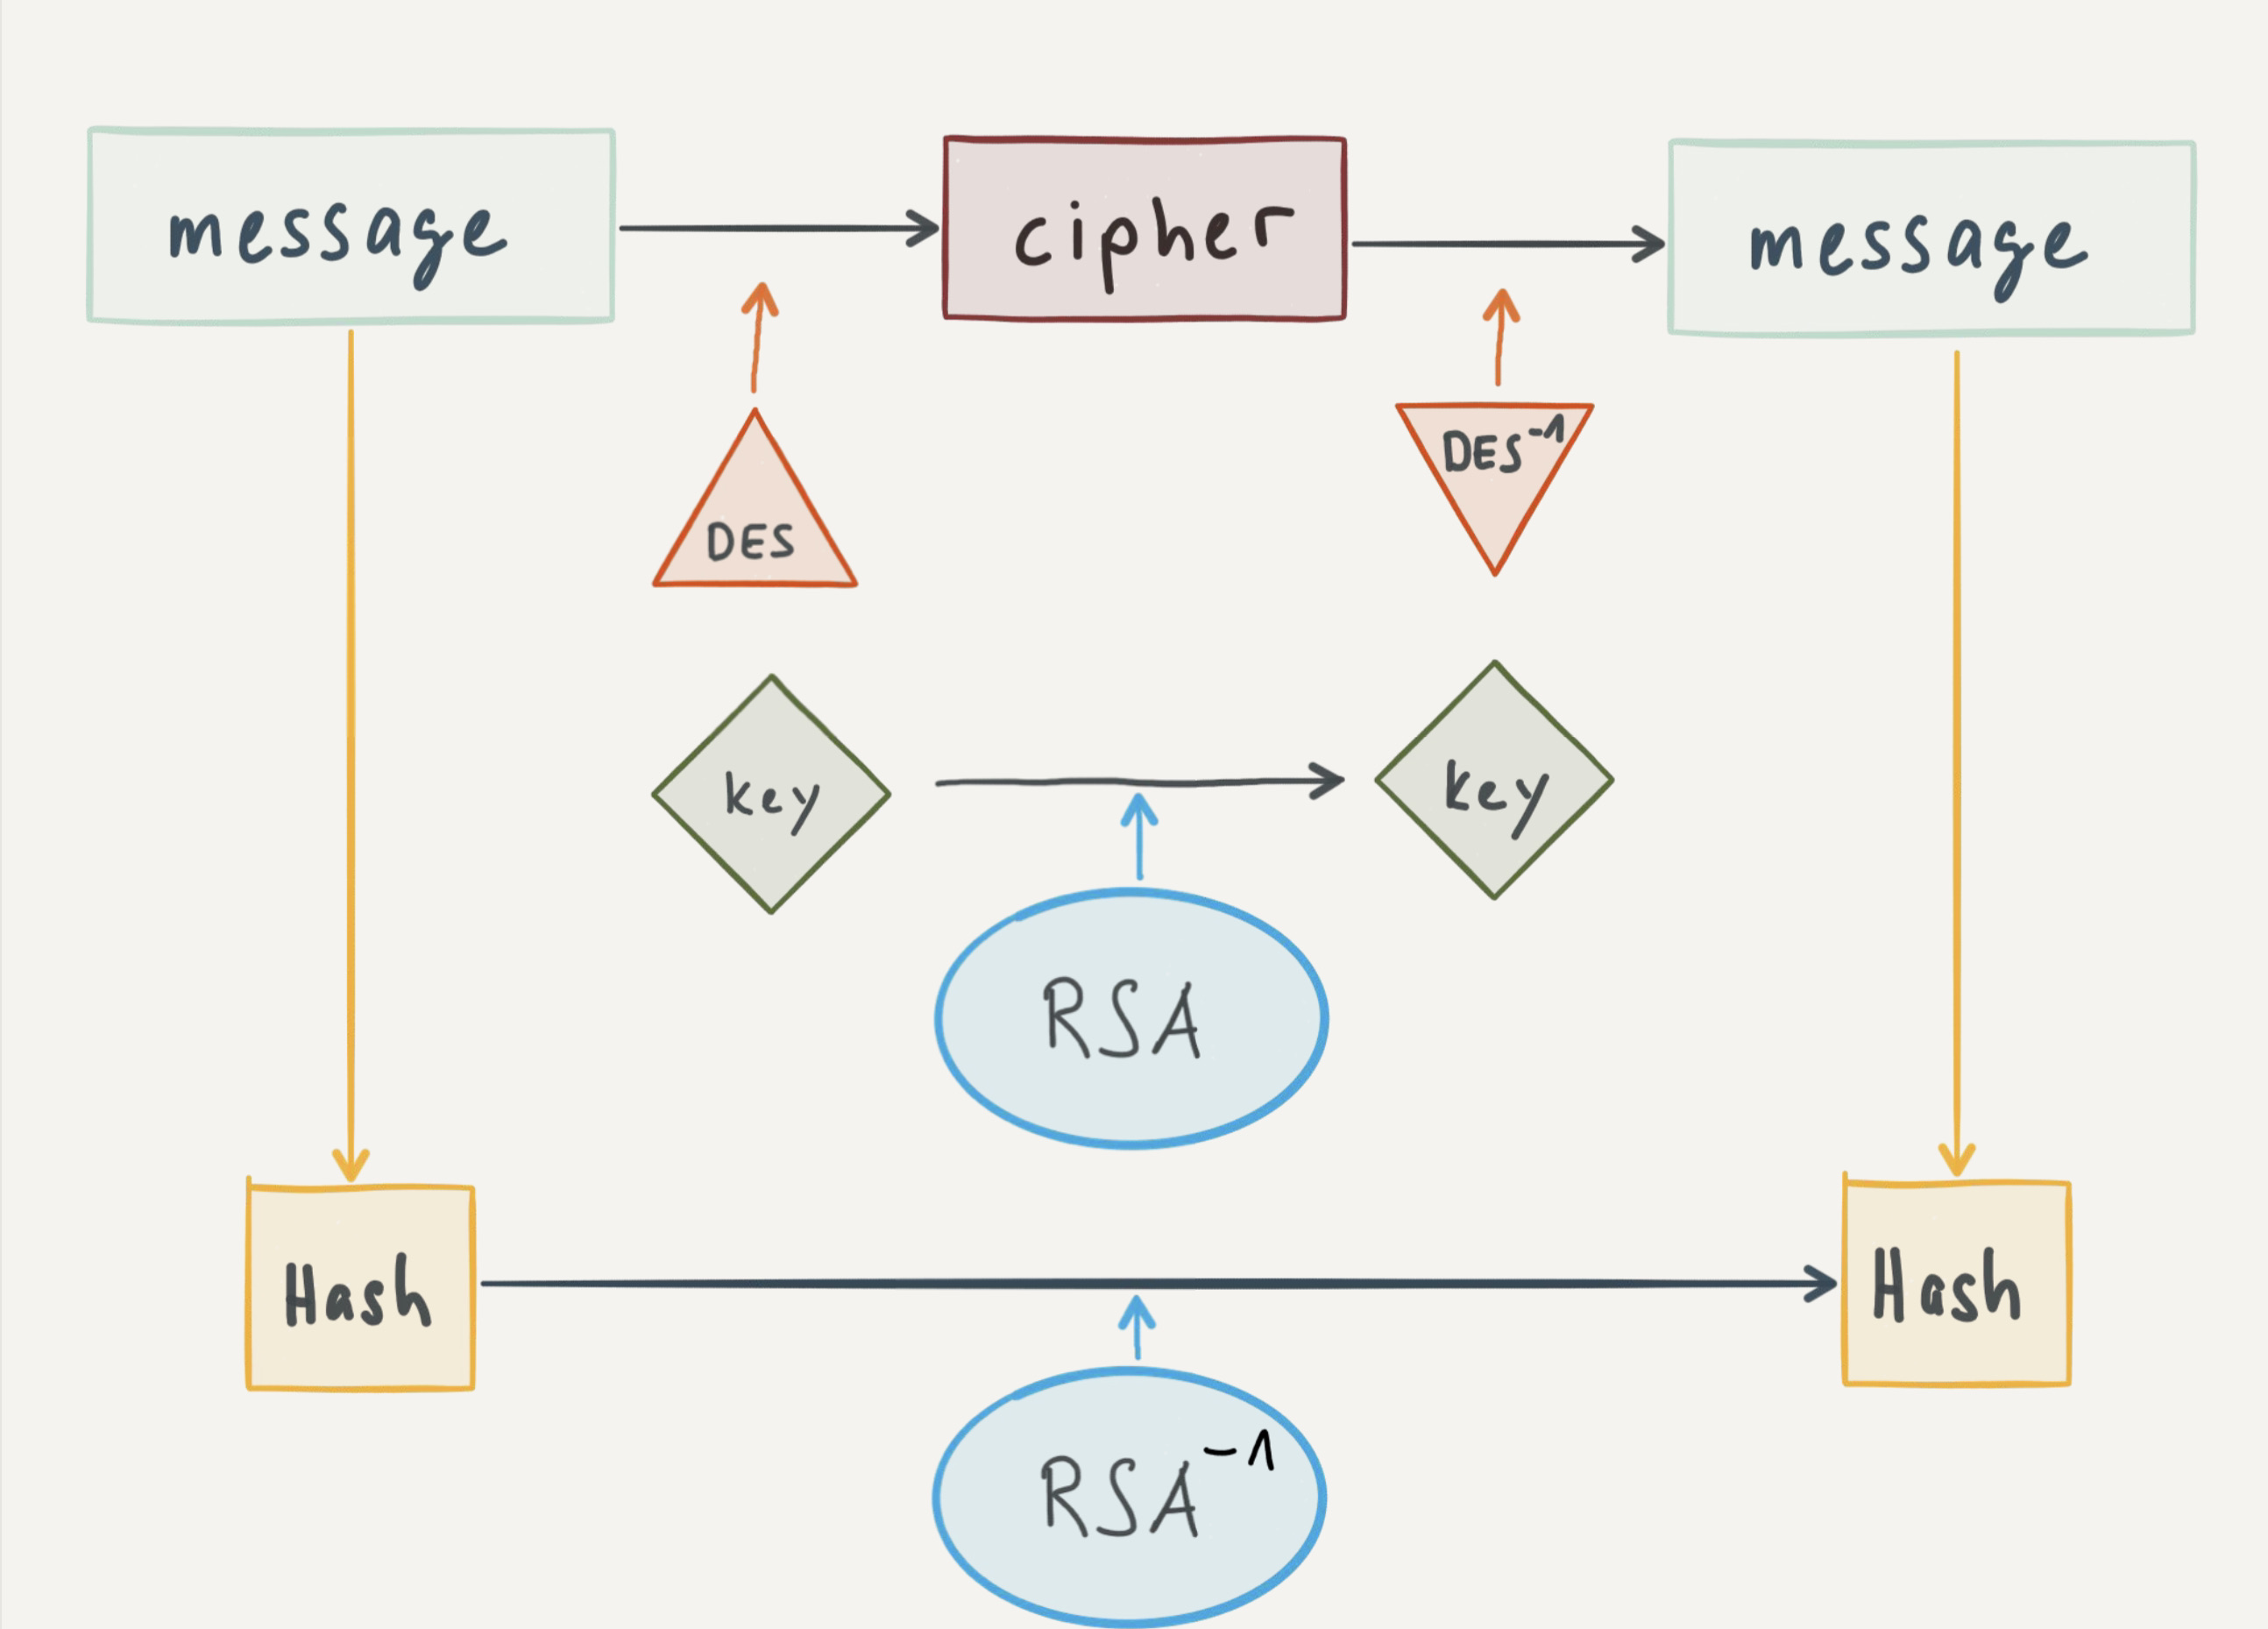
\includegraphics[width=0.4\textwidth]{pictures/pgpscheme.jpeg}
    \caption{PGP Schema}
    \label{fig:pgp}
\end{figure}
Bei mir hier im Unterricht simulieren wir das Verfahren mit RSA und verwenden als Hash/Fingerprint die check-digit aus der ISBN-10 Nummer aus dem Abschnitt Barcode.

\clearpage

\appendix

\section{Memorandum Bombes}
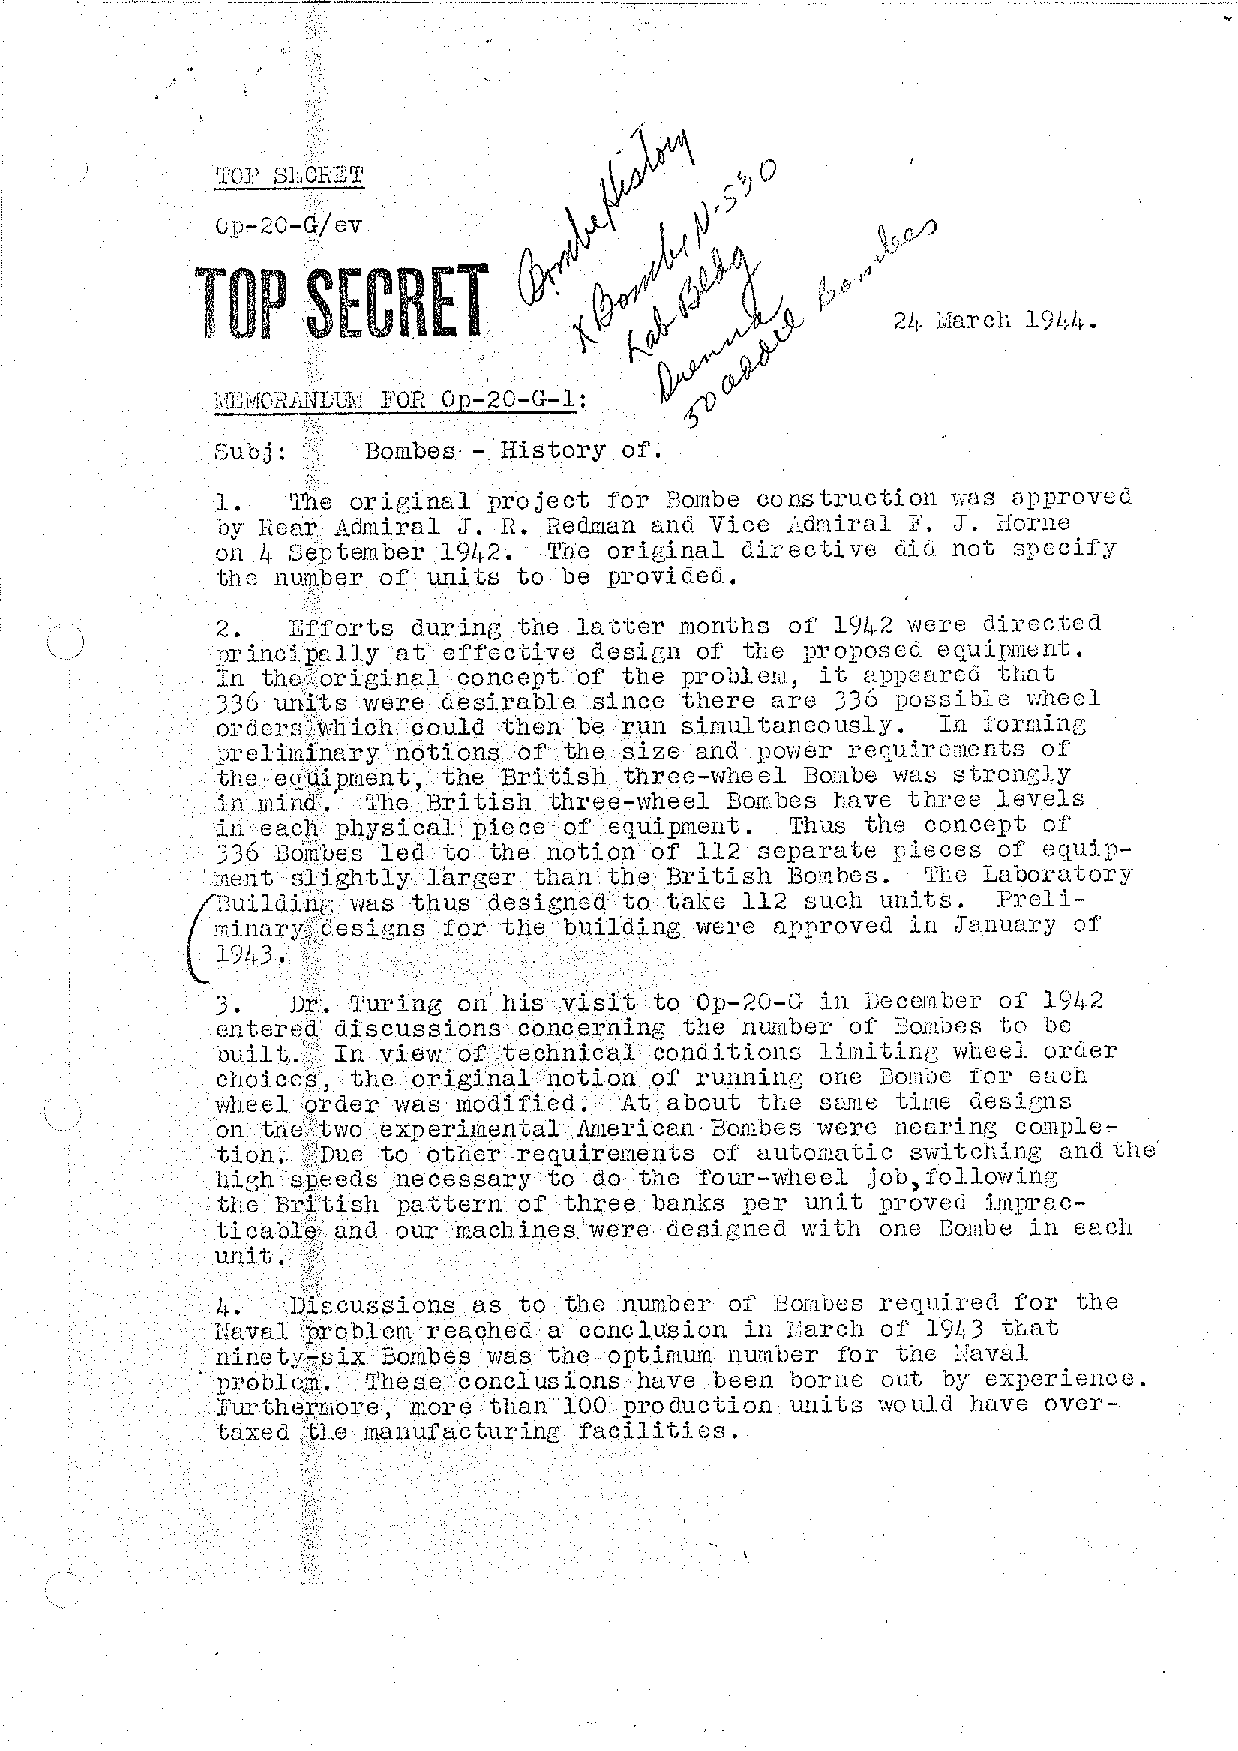
\includegraphics[width=0.88\textwidth,page=1]{pictures/memorandumbombes.pdf}

\includegraphics[width=1\textwidth,page=2]{pictures/memorandumbombes.pdf}

\cleardoublepage
\listoffigures
\listoftables
%\newpage
%\nocite{*}
%\bibliographystyle{plain}
%\bibliography{preamble/literaturgoogle}
\end{document}